\documentclass{article}
%
%\usepackage{amsmath}
%\usepackage{amssymb}
%\usepackage{graphics}
%
\usepackage{graphicx}                              %for PNG images
\usepackage{color}                                 %for defining custom colors
\usepackage{framed}                                %for shaded and framed paragraphs
%\usepackage{makeidx}                               %for index page
\usepackage{geometry}                              %for defining page size
\usepackage[linkbordercolor={0 0.8 0.8}]{hyperref} %for \url tag
%
\geometry{verbose,a4paper,tmargin=2.5cm,bmargin=2.5cm,lmargin=2.5cm,rmargin=2cm}
\makeindex
\hypersetup{
  pdfauthor = {Balazs Konya},
  pdftitle = {ARC Information System},
  pdfsubject = {Technical description},
  pdfkeywords = {Grid,NorduGrid,information systems},
  pdfcreator = {PDFLaTeX with hyperref package},
  pdfproducer = {PDFLaTeX}
}
%
%\bibliographystyle{IEEEtran}
%
\def\efill{\hfill\nopagebreak}%
\hyphenation{Nordu-Grid}
\setlength{\parindent}{0cm}
\setlength{\FrameRule}{1pt}
\setlength{\FrameSep}{8pt}
\addtolength{\parskip}{5pt}
\renewcommand{\thefootnote}{\fnsymbol{footnote}}
\renewcommand{\arraystretch}{1.3}
\newcommand{\dothis}{\colorbox{shadecolor}}
\newcommand{\gt}{Globus Toolkit$\mathrm{^{TM}}$}
\definecolor{shadecolor}{rgb}{1,1,0.6}
\definecolor{salmon}{rgb}{1,0.9,1}
\definecolor{cyan}{rgb}{0,1,1}

\begin{document}
  \def\today{\number\day/\number\month/\number\year}
  
  \begin{titlepage}
    
    \begin{tabular}{rl}
      \resizebox*{3cm}{!}{
\includegraphics{ng-logo.png}}
      &\parbox[b]{2cm}{\textbf \it {\hspace*{-1.5cm}NORDUGRID\vspace*{0.5cm}}}
    \end{tabular}
    
    \hrulefill
    
    {\raggedleft NORDUGRID-TECH-4\par}
    
    {\raggedleft \today\par}
    
    \vspace*{2cm}
    
%%%%---- The title ----
    {\centering \textsc{\Large The NorduGrid/ARC Information System}\Large \par}
    
    \vspace*{0.5cm}
    
%%%%---- A subtitle, if necessary ----
    {\centering \textit{\large Technical Description and Reference Manual}\large \par}
    
    \vspace*{2cm}
			
%%%%---- A list of authors ----
    {\centering \large Bal\'azs K\'onya\footnote{Comments to:
     balazs.konya@hep.lu.se} \large \par}
    
    \vspace*{3.5cm}

			
    {\centering \large %Refers to ARC release series 0.4 and up 
    \it Version 0.9
    \large \par}
        
%%%%---- An abstract ----
%\begin{abstract}

%\end{abstract}

\end{titlepage}
\thispagestyle{empty} $ $
\newpage
$\ $

%%%%---- Table of Contents, uncomment if necessary
%\tableofcontents{}


%TODO make clear what is available in which arc-version, mention 0.5 
% as a pre-0.6

\section{Introduction}

A stable, robust, scalable, dynamic and reliable information system is
a cornerstone of any kind of Grid system. Without a properly working
information system it is not possible to construct a production
quality Grid. A scalable Grid information system is inherently
distributed, a centralized system is not able to cope with the
dynamism of the Grid.


The information system acts as a nervous system of the Grid and its
main tasks consist of
\begin{itemize}
\item Resource Description:
Characterization of Grid resources by specifying static, semi-static
and dynamic properties (e.g. information about Grid jobs and user
quotas are presented as dynamic local resource properties).

Grid clients are relying on the resource description functionality of
the information system during their matchmaking and brokering
process. Grid monitoring and job status queries also rely on resource
description.

\item Resource aggregation:
Individual resources are connected to an "information mesh" by
dynamically registering to some of the information index services. The
information index services are responsible for the resource
aggregation, they maintain a dynamic list of available Grid resources.
Furthermore, the index services are connected to each other following
a specific topological order. The resulting structure is the
"information mesh" of the Grid.

Grid clients performing resource discovery scan the '"information
mesh" utilizing its topological structure in order to find available
Grid resources.  Therefore resource discovery is delicately coupled to
the topological structure of the "information mesh" that is to the
resource aggregation process.
\end{itemize}

The ARC middleware implements a scalable, production quality
dynamic distributed information system. The ARC information system 
has been deployed and being used in a large scale production environment 
since May 2002. As of writing, the information system aggregates ~70 
resources providing \gt 40 thousand CPUs and serves \gt 400 thousand jobs per month.

The ARC information system is an OpenLDAP-based system\cite{Openldap}
which is derived from the Globus Monitoring and Discovery Services
framework \cite{mds}. It uses BDII\cite{bdii} together with a updated MDS LDAP Schema.


This document presents a technical overview of the ARC Grid information system. 
The document describes the architecture, the implementation of the main components 
and the NorduGrid/ARC Information model. The document is also intended to serve as  
reference manual by giving a detailed description of the available Grid information.


\section{Overview}

The ARC middleware implements a dynamic LDAP-based distributed information 
system via set of coupled resource lists (index services) and 
local LDAP databases. The system consists of three main components:
\begin{enumerate}
\item the Local Information Trees (LIT),
\item the Index Services  (IS),
\item and the Registration Processes (RP)
\end{enumerate}

The local information trees are responsible for resource (computing or storage)
description and characterization. The local information is generated on the 
resource, optionally it is cached. Upon client requests it is presented to the 
clients via LDAP interface.
 
The main task of the index services is to maintain a dynamic list of resources 
(LDAP URLs of the local information trees) and index services. 
The index services are further coupled together implementing a specific topology. 

The local information trees make use of the registration processes
running locally on the resources in order to list themselves in some of the 
resource lists maintained by the index services. Registrations are always 
initiated by the registrants (bottom-up model).

Grid clients such as monitors, web portals or user interfaces
perform two type of queries:
\begin{enumerate}
\item During the resource discovery process
clients query index services in order to collect list of LDAP contact 
URLs of local information trees describing Grid-connected resources. 


\item
During a direct resource query the clients directly contact the 
local information tree by making use of the obtained LDAP contact URLs.
\end{enumerate}

Both type of queries are carried out and served via LDAP protocol.

Figure~\ref{fig:overview} presents an overview of the ARC information system
components.


\begin{figure}[hb]
\centering
{ 
{\scalebox{0.35}{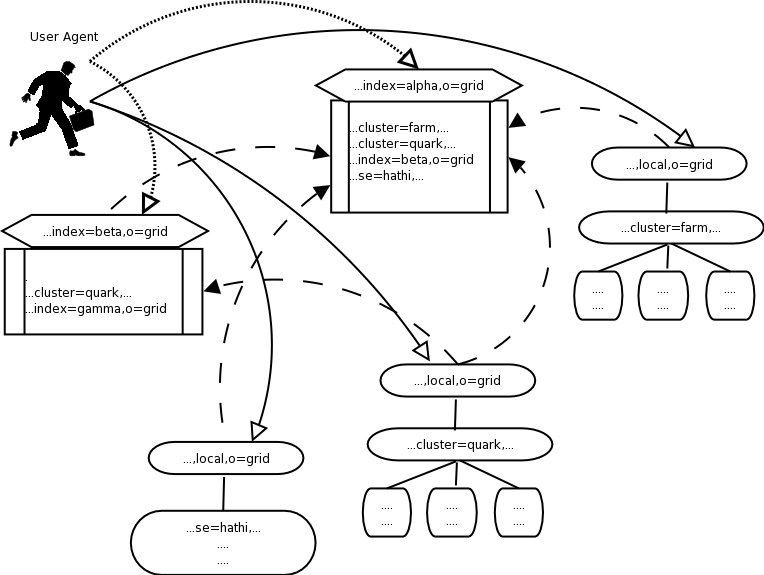
\includegraphics{infosys_overview.png}}}
}
\caption{\label{fig:overview}Overview of the ARC information system components.}
\end{figure}


\section{Local Information Tree}

The LIT component of the information system is responsible
for generating the dynamic state information, implementing the first-level caching
of the local information and providing the requested Grid information to the clients 
through the LDAP protocol. The LIT is basically nothing more but a 
specially populated and customized OpenLDAP database.

The dynamic resource state information is generated on the resource.
Small and efficient programs, called information providers, are used to 
collect local state information from the batch system, from the local Grid layer 
(e.g. Grid Manager or GridFTP server \cite{grid-manager}) or from the
local operating system (e.g. information available in the \texttt{/proc} area).
Currently, ARC is capable interfacing to the following batch systems 
(or local resource management system LRMS in the ARC terminology): 
UNIX fork, the PBS-family (OpenPBS, PBS-Pro, Torque), Condor, Sun Grid Engine, IBM LoadLeveler and SLURM.  

The output of the information providers (generated in LDIF format) is
used to populate the local LDAP tree. This OpenLDAP back-end
implements two things: it is capable caching the providers output and
upon client query request it triggers the information providers unless
the data is already available in its cache.  The caching feature of
the OpenLDAP back-end provides protection against overloading the
local resource by continuously triggering the information providers.

The information stored in the LIT follows the NorduGrid-ARC
information model.  The section \ref{sec:infomodel} gives a detailed
technical account of the ARC information model.

\subsection{Security considerations}

The Local Information Tree is implemented via an LDAP database which implies the security and
confidentiality capabilities of the system. 

OpenLDAP\cite{Openldap} contains two methods for specifying access control. 
The first is static, i.e. you define the rights in configuration files.
From an operational point of view, the problem of this method is that needs a 
server restart at every security configuration change.
The second method for access control, called as ACI (Access Control Information), 
inserts access control information inside the directory itself by augmenting 
every LDAP entry with a dynamically  modifiable ACL.
Unfortunately the ACI method is still considered to be experimental.

The current ARC setup makes use of the static LDAP access control, the trees are 
configured to be fully readable by anybody: ARC provides  anonymous read
access to every information stored in the local trees.

There are considerations to experiment with the ACI access control method  
or to modify the static configuration and require authentication
from the clients.


\section{The ARC information model \label{sec:infomodel}}

A Grid information model should be a result of a
delicate design process how to represent the resources and what is
the best way to structure this information. 

ARC implements an LDAP-based information system. In an LDAP-based system the 
information is being stored as attribute-value pairs grouped 
together in entries which are organized into a hierarchical tree.
Therefore an LDAP-based information model is technically specified via 
an LDAP schema AND the structure of the LDAP-tree (DIT).


The ARC information model naturally describes the main Grid
components:
\begin{itemize} 
\item computing resources with Grid jobs and Grid users, 
\item storage elements,
\item and metadata catalogues
\end{itemize}
though the latter two are treated in a rather simplistic
manner.  

\subsection{LDAP technicalities: namespace, OID, objectclasses, attributes}

The NorduGrid/ARC LDAP schema (available in appendix~\ref{appendix:schema})
makes use of the {\it nordugrid-} namespace, the objectclass
and attribute names starts with the {\it nordugrid-} prefix.

NorduGrid is assigned to the {\mbox 1.3.6.1.4.1.11604} Private Enterprise Number 
which is utilized according to the Table\ref{Table:OID1}.

%this is turned into a table
% 1.3.6.1.4.1.11604.1 security
% 1.3.6.1.4.1.11604.2 info
% 1.3.6.1.4.1.11604.3 data management
% 1.3.6.1.4.1.11604.4 user management

\providecommand{\tabularnewline}{\\}

\begin{table}
\centering
\begin{tabular}{|l|c|}
\hline
Object Identifier&
Service area\tabularnewline
\hline
\hline
1.3.6.1.4.1.11604.1&
security\tabularnewline
\hline
1.3.6.1.4.1.11604.2&
information system\tabularnewline
\hline
1.3.6.1.4.1.11604.3&
data management\tabularnewline
\hline
1.3.6.1.4.1.11604.4&
user management\tabularnewline
\hline
\end{tabular}
\caption{\label{Table:OID1} The OID space utilization within ARC}
\end{table}


The OID's used in the LDAP schema are shown in 
Table\ref{Table:OID2} and are taken from the range {\mbox 1.3.6.1.4.1.11604.2.*}
Table\ref{Table:OID2} also serves as a list of the NorduGrid objectclasses.
The ARC implementation follows a "one LDAP entry = one objectclass" approach,
The ARC information system objects such as Grid-enabled clusters, queues, storages, 
Grid users and Grid jobs are described by specific LDAP entry which utilizes
a single objectclass. As a result a one-to-one correspondence exists between
ARC LDAP entries and ARC objectclasses.

The detailed description of the objectclasses and attributes 
are given in the following subsections. First the main purpose  
behind the objectclass is outlined followed by the one-by-one 
description of the attributes. The attribute descriptions also contain 
information about the attributes role played in the brokering\cite{arc_brokering},
the job submission or the monitoring process. If applicable, the corresponding 
xRSL attribute\cite{xrsl_manual} is displayed. 
Please notice that the most of the attribute values documented below are not enforced, 
misconfigured or rough sites can publish incorrect information.

%TODO: think of attribute default values, unset/irrelevant attributes 


%this is turned into a table
%1.3.6.1.4.1.11604.2.1.1  	cluster objectclass
%1.3.6.1.4.1.11604.2.1.1.x	cluster attributes
%1.3.6.1.4.1.11604.2.1.2  	nordugrid-info-group objectclass
%1.3.6.1.4.1.11604.2.1.2.x	nordugrid-info-group attributes
%1.3.6.1.4.1.11604.2.1.3  	nordugrid-queue objectclass
%1.3.6.1.4.1.11604.2.1.3.x 	nordugrid-queue attributes
%1.3.6.1.4.1.11604.2.1.4  	nordugrid-job
%1.3.6.1.4.1.11604.2.1.4.x	nordugrid-job attributes
%1.3.6.1.4.1.11604.2.1.5  	nordugrid-authuser
%1.3.6.1.4.1.11604.2.1.5.x	nordugrid-authuser attributes
%1.3.6.1.4.1.11604.2.1.6  	nordugrid-se
%1.3.6.1.4.1.11604.2.1.6.x	nordugrid-se attributes
%1.3.6.1.4.1.11604.2.1.7  	nordugrid-rc
%1.3.6.1.4.1.11604.2.1.7.x	nordugrid-rc attributes
%1.3.6.1.4.1.11604.2.1.7  	mds
%1.3.6.1.4.1.11604.2.1.7.x	mds attributes


\begin{table}
\centering
\begin{tabular}{|l|c|}
\hline 
1.3.6.1.4.1.11604.2.1.1&
cluster objectclass\tabularnewline
\hline 
1.3.6.1.4.1.11604.2.1.1.x&
cluster attributes\tabularnewline
\hline 
1.3.6.1.4.1.11604.2.1.2&
info-group objectclass\tabularnewline
\hline 
1.3.6.1.4.1.11604.2.1.2.x&
info-group attributes\tabularnewline
\hline 
1.3.6.1.4.1.11604.2.1.3 &
queue objectclass\tabularnewline
\hline 
1.3.6.1.4.1.11604.2.1.3.x&
queue attributes\tabularnewline
\hline 
1.3.6.1.4.1.11604.2.1.4&
job objectclass\tabularnewline
\hline 
1.3.6.1.4.1.11604.2.1.4.x&
job attributes\tabularnewline
\hline 
1.3.6.1.4.1.11604.2.1.5&
authuser objectclass\tabularnewline
\hline 
1.3.6.1.4.1.11604.2.1.5.x&
authuser attributes\tabularnewline
\hline 
1.3.6.1.4.1.11604.2.1.6&
se objectclass\tabularnewline
\hline 
1.3.6.1.4.1.11604.2.1.6.x&
se attributes\tabularnewline
\hline 
1.3.6.1.4.1.11604.2.1.7 &
rc objectclass\tabularnewline
\hline 
1.3.6.1.4.1.11604.2.1.7.x&
rc attributes\tabularnewline
\hline 
1.3.6.1.4.1.11604.2.1.8 &
Mds objectclass\tabularnewline
\hline 
1.3.6.1.4.1.11604.2.1.8.x&
Mds attributes\tabularnewline
\hline 
\end{tabular}
\caption{\label{Table:OID2} The OIDs from the NorduGrid/ARC schema}
\end{table}



\subsection{The structure of the local LDAP tree: Arc DIT}


The ARC local LDAP tree gives a natural representation 
of a Grid-enabled resource. 
The {\it mds-vo-name=local,o=grid} top level entry of the tree
carries no information, its role is purely structural. This entry
accommodates the subtrees of the different Grid services offered by the 
local machine. A Grid resource in ARC can host a computing service 
and several storage or data indexing services. A computing service is 
described by the cluster subtree, while the storage and data indexing services 
are characterised by the {\it se} and {\it rc} single-entry subtrees, respectively.

%
%TODO add a paragraph about the useability, performance implication of a bad DIT
% design

\begin{figure}[hb]
\centering
{ {\scalebox{0.4}{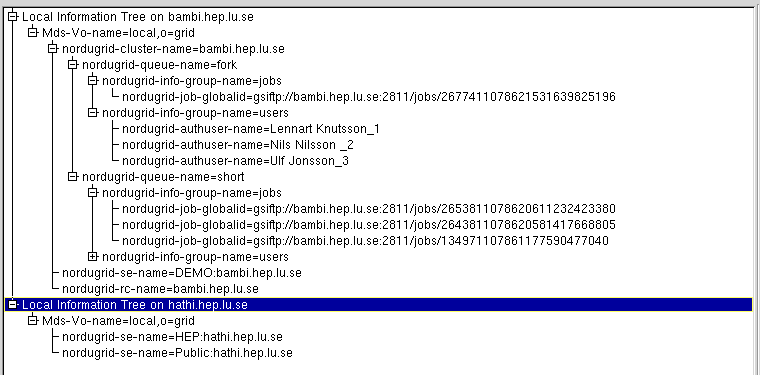
\includegraphics{lit.png}}} }
\caption{\label{fig:dit} The local information tree on two resources. 
The first machine bambi.hep.lu.se provides both computing, storage and data indexing services
while the second resource hathi.hep.lu.se hosts two storage elements.}
\end{figure} 

Figure~\ref{fig:dit} shows the local LDAP tree of two Grid-enabled resources.
The first machine bambi.hep.lu.se offers both a computing service,
a storage service and a data indexing service, therefore the LIT of bambi.hep.lu.se
contains a cluster subtree under the {\it nordugrid-cluster-name=bambi.hep.lu.se} entry 
a storage {\it nordugrid-se-name=..} and a data indexing {\it nordugrid-rc-name=...}
entry. The second resource hathi.hep.lu.se serves as a dedicated storage hosting two storage
elements, therefore the LIT of hathi.hep.lu.se consists of the two storage entries. 


The schematic structure of the cluster subtree is shown enlarged in 
Fig.~\ref{fig:dit_subcluster}. The {\it cluster} top entry of the 
subtree describes the hardware, software and middleware
properties of a cluster. Grid-enabled queues are represented by their 
{\it queue} entries. Active Grid jobs and authorized Grid users are 
described by their corresponding {\it job} and {\it authuser} 
entries which are located under their hosting queues.
The {\it job} and {\it authuser} entries belonging to the same 
queue are grouped in two distinct subtrees,
the branching is accomplished by structural {\it nordugrid-info-group=job} 
and {\it nordugrid-info-group=user} entries.

The storage and data indexing services are represented by their corresponding
single LDAP entries, currently no LDAP subtree is associated to them.

\begin{figure}[hb]
\centering
{ {\scalebox{0.4}{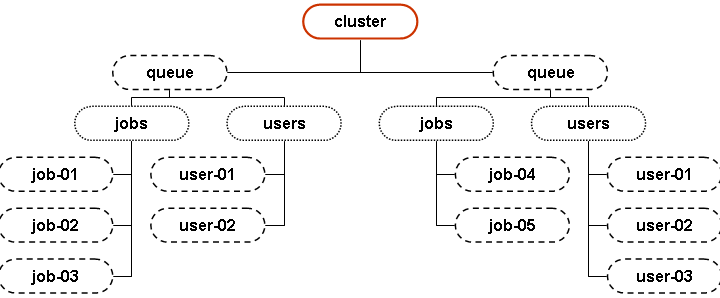
\includegraphics{cluster_dit.png}}} }
\caption{\label{fig:dit_subcluster} The schematic picture of an LDAP subtree representing a
computing resource. The cluster subtree is part of the LIT shown in Fig:~\ref{fig:dit}}
\end{figure} 


\subsection{Globus Mds}
These are the globus-mds attributes that we have incorporated into
arc.  The schema contains special objectclasses: {\it Mds}, 
{\it MdsVo}, {\it MdsVoName}, {\it MdsServiceLdap} and {\it MdsService}
whose role it is to create structural entries in the LDAP tree.

\phantomsection
  \addcontentsline{toc}{subsubsection}{mds-validfrom}
  \hspace*{0.5cm}
  \begin{shaded}
    \textbf{mds-validfrom}
  \end{shaded}
  \begin{tabular}{lp{10cm}}  
    Attribute value:&\verb# {time}#\\
    Example: &\verb# 20050307103026Z#\\
    Related xRSL:&none \\
  \end{tabular}

\phantomsection
  \addcontentsline{toc}{subsubsection}{mds-validto}
  \hspace*{0.5cm}
  \begin{shaded}
    \textbf{mds-validto}
  \end{shaded}
  \begin{tabular}{lp{10cm}}  
    Attribute value:&\verb# {time}#\\
    Example: &\verb# 20050307103026Z#\\
    Related xRSL:&none \\
  \end{tabular}

\phantomsection
  \addcontentsline{toc}{subsubsection}{mds-keepto}
  \hspace*{0.5cm}
  \begin{shaded}
    \textbf{mds-keepto}
  \end{shaded}
  \begin{tabular}{lp{10cm}}  
    Attribute value:&\verb# {time}#\\
    Example: &\verb# 20050307103026Z#\\
    Related xRSL:&none \\
  \end{tabular}

\phantomsection
  \addcontentsline{toc}{subsubsection}{mds-vo-name}
  \hspace*{0.5cm}
  \begin{shaded}
    \textbf{mds-vo-name}
  \end{shaded}
  \begin{tabular}{lp{10cm}}  
    Attribute value:&\verb# {Locally unique VO name}#\\
    Example: &\verb# local #\\
    Related xRSL:&none \\
  \end{tabular}

\phantomsection
  \addcontentsline{toc}{subsubsection}{mds-vo-op-name}
  \hspace*{0.5cm}
  \begin{shaded}
    \textbf{mds-vo-op-name}
  \end{shaded}
  \begin{tabular}{lp{10cm}}  
    Attribute value:&\verb# {Locally unique Op name}#\\
    Related xRSL:&none \\
  \end{tabular}

\phantomsection
  \addcontentsline{toc}{subsubsection}{mds-service-type}
  \hspace*{0.5cm}
  \begin{shaded}
    \textbf{mds-service-type}
  \end{shaded}
  \begin{tabular}{lp{10cm}}  
    Attribute value:&\verb# {Mds service type}#\\
    Example: &\verb# ldap #\\
    Related xRSL:&none \\
  \end{tabular}

\phantomsection
  \addcontentsline{toc}{subsubsection}{mds-service-protocol}
  \hspace*{0.5cm}
  \begin{shaded}
    \textbf{mds-service-protocol}
  \end{shaded}
  \begin{tabular}{lp{10cm}}  
    Attribute value:&\verb# {Service protocol OID}#\\
    Related xRSL:&none \\
  \end{tabular}

\phantomsection
  \addcontentsline{toc}{subsubsection}{mds-service-port}
  \hspace*{0.5cm}
  \begin{shaded}
    \textbf{mds-service-port}
  \end{shaded}
  \begin{tabular}{lp{10cm}}  
    Attribute value:&\verb# {Service TCP port}#\\
    Related xRSL:&none \\
  \end{tabular}

\phantomsection
  \addcontentsline{toc}{subsubsection}{mds-service-hn}
  \hspace*{0.5cm}
  \begin{shaded}
    \textbf{mds-service-hn}
  \end{shaded}
  \begin{tabular}{lp{10cm}}  
    Attribute value:&\verb# {Service FQDN hostname}#\\
    Related xRSL:&none \\
  \end{tabular}

\phantomsection
  \addcontentsline{toc}{subsubsection}{mds-service-url}
  \hspace*{0.5cm}
  \begin{shaded}
    \textbf{mds-service-url}
  \end{shaded}
  \begin{tabular}{lp{10cm}}  
    Attribute value:&\verb# {Service URL}#\\
    Related xRSL:&none \\
  \end{tabular}

\phantomsection
  \addcontentsline{toc}{subsubsection}{mds-service-ldap-suffix}
  \hspace*{0.5cm}
  \begin{shaded}
    \textbf{mds-service-ldap-suffix}
  \end{shaded}
  \begin{tabular}{lp{10cm}}  
    Attribute value:&\verb# {DN suffix of service}#\\
    Example: &\verb# Mds-Vo-Name=local, o=grid #\\
    Related xRSL:&none \\
  \end{tabular}

\phantomsection
  \addcontentsline{toc}{subsubsection}{mds-service-ldap-timeout}
  \hspace*{0.5cm}
  \begin{shaded}
    \textbf{mds-service-ldap-timeout}
  \end{shaded}
  \begin{tabular}{lp{10cm}}  
    Attribute value:&\verb# {time in minutes}#\\
    Related xRSL:&none \\
  \end{tabular}

\phantomsection
  \addcontentsline{toc}{subsubsection}{mds-service-ldap-sizelimit}
  \hspace*{0.5cm}
  \begin{shaded}
    \textbf{mds-service-ldap-sizelimit}
  \end{shaded}
  \begin{tabular}{lp{10cm}}  
    Attribute value:&\verb# {size}#\\
    Related xRSL:&none \\
  \end{tabular}

\phantomsection
  \addcontentsline{toc}{subsubsection}{mds-service-ldap-cachettl}
  \hspace*{0.5cm}
  \begin{shaded}
    \textbf{mds-service-ldap-cachettl}
  \end{shaded}
  \begin{tabular}{lp{10cm}}  
    Attribute value:&\verb# {time in minutes}#\\
    Related xRSL:&none \\
  \end{tabular}

\phantomsection
  \addcontentsline{toc}{subsubsection}{mds-sercice-ldap-ttl}
  \hspace*{0.5cm}
  \begin{shaded}
    \textbf{mds-service-ldap-ttl}
  \end{shaded}
  \begin{tabular}{lp{10cm}}  
    Attribute value:&\verb# {time in minutes}#\\
    Related xRSL:&none \\
  \end{tabular}

\phantomsection
  \addcontentsline{toc}{subsubsection}{mds-reg-status}
  \hspace*{0.5cm}
  \begin{shaded}
    \textbf{mds-reg-status}
  \end{shaded}
  \begin{tabular}{lp{10cm}}  
    Attribute value:&\verb# {status}#\\
    Example: &\verb# VALID #\\
    Related xRSL:&none \\
  \end{tabular}

\phantomsection
  \addcontentsline{toc}{subsubsection}{mds-bind-method-servers}
  \hspace*{0.5cm}
  \begin{shaded}
    \textbf{mds-bind-method-servers}
  \end{shaded}
  \begin{tabular}{lp{10cm}}  
    Attribute value:&\verb# {type of server}#\\
    Example: &\verb# ANONYM-ONLY #\\
    Related xRSL:&none \\
  \end{tabular}

\subsection{Grouping authuser and job entries: nordugrid-info-group objectclass}

The schema contains a special objectclass the {\it nordugrid-info-group}
whose role is to create structural entries in the LDAP tree.
The entries {\it nordugrid-info-group=jobs} and {\it nordugrid-info-group=users}
of the LIT are separating nordugrid-job and nordugrid-authuser entries of a 
grid queue by grouping them in two
separate LDAP branches under the queue entry (see Fig.~\ref{fig:dit} ).  

The objectclass comes with a single attribute.

\phantomsection
  \addcontentsline{toc}{subsubsection}{nordugrid-info-group-name}
  \hspace*{0.5cm}
  \begin{shaded}
    \textbf{nordugrid-info-group-name}
  \end{shaded}
  \begin{tabular}{lp{10cm}}  
    Attribute value:&\verb# {users,jobs}#\\
    Related xRSL:&none \\
  \end{tabular}

The {\it nordugrid-info-group-name} attribute
is used to distinguish between jobs or users grouping:
nordugrid-job entries are grouped under the structural entry 
{\it nordugrid-info-group-name=jobs} while nordugrid-authuser entries are
grouped under the {\it nordugrid-info-group-name=users} entry.


\subsection{Computing resources: nordugrid-cluster and nordugrid-queue objectclass}
\label{section:cluster-queue}

The nordugrid schema provides two objectclasses for the description of 
a computing resource. The {\it nordugrid-cluster} is used to describe 
general properties such as ownership, name, location, contact URL, 
pre-installed software environments, Grid scratch space, batch system,
node properties such as architecture, CPUs, network connectivity. 
Dynamic cluster load information, such as number of queued/total jobs, 
is also part of the objectclass information.

The generalized concept of a 
computing queue plays a central role in ARC:
queues are the job submission targets in an ARC-based Grid, during the brokering
process clients select a Grid-enabled queue on a computing resource.
An ARC queue represents either a traditional batch queue of a local resource management
system (LRMS) such as the PBS or describes an entire LRMS when the 
LRMS does not support conventional queues
(Condor and SGE is handled this way). The very special  LRMS, the UNIX fork
is also described as queue. 
The {\it nordugrid-queue} objectclass is designed to describe the generalized concept of
a computing queue. Besides the usual queue-specific information (queue status
and limits, number of running/queueing jobs)  queue-level node attributes are also 
introduced to describe hardware/software 
characteristics of computing nodes assigned to a certain queue.  
Also notice that the schema makes possible the 
distinction of Grid and non-grid jobs being managed by the queue.


The ARC schema introduces cluster- and queue-level node attributes
together with two homogeneity attributes
in order to handle possible inhomogeneity within a computing resource.
The schema is designed to be capable describing inhomogeneous resources with a
queue-level homogeneity assumption but higher level inhomogeneity
can also be treated with less accuracy.

In case of homogeneous nodes the {\it nordugrid-cluster-homogeneity=true}
is set and the cluster-level node attributes carry the relevant information.
If the nodes are inhomogeneous the {\it nordugrid-cluster-homogeneity=no}
is set and the cluster-level node attributes are either not set or
their value refers to the smallest/slowest/least powerful node.
Suppose the nodes can be organized into homogeneous subgroups, 
this case the queue-level node attributes are used to 
describe the properties of the homogeneous nodes
assigned to the same queue. Clients should always treat the 
queue-level node attributes with higher priority than the 
cluster-level ones. The {\it nordugrid-queue-homogeneity=true}
attribute value is used to specify the node homogeneity within a queue.
The {\it nordugrid-queue-homogeneity=no} means that if 
a given queue-level node attribute is set it
refers to the smallest/slowest/least powerful node.



\phantomsection
  \addcontentsline{toc}{subsubsection}{nordugrid-cluster-name}
  \hspace*{0.5cm}
  \begin{shaded}
    \textbf{nordugrid-cluster-name}
  \end{shaded}
  \begin{tabular}{lp{10cm}}  
    Attribute value:& FQDN\\
    Example:&  \verb#nordugrid-cluster-name: gate1.monstercluster.nordugrid.org#\\
    Related xRSL:& \verb#cluster#\\
    UI role:& used in matchmaking, monitoring, job manipulation \\
    
  \end{tabular}

Description: The fully qualified domain name of the front-end machine of the 
cluster. This attribute is used in the Distinguished Name of a cluster LDAP entry.

%DISCUSS several computing resource running on the same box: what makes the 
% cluster-name unique?

\phantomsection
  \addcontentsline{toc}{subsubsection}{nordugrid-cluster-aliasname}
  \hspace*{0.5cm}
  \begin{shaded}
    \textbf{nordugrid-cluster-aliasname}
  \end{shaded}
  \begin{tabular}{lp{10cm}}  
    Attribute value:& free form text\\
    Example:& \verb#nordugrid-cluster-aliasname: Grid Monster#\\
    Related xRSL:& none\\
    UI role:& ?\\
  \end{tabular}

Description: A free form text attribute displaying the alias name of the computing resource.


\phantomsection
  \addcontentsline{toc}{subsubsection}{nordugrid-cluster-contactstring}
  \hspace*{0.5cm}
  \begin{shaded}
    \textbf{nordugrid-cluster-contactstring}
  \end{shaded}
  \begin{tabular}{lp{10cm}}  
    Attribute value:& URL\\
    Example:& \verb#nordugrid-cluster-contactstring: gsiftp://bambi.hep.lu.se:2811/jobs#\\
    Related xRSL:& none\\    
    UI role:& used during the job submission process\\
  \end{tabular}

Description: The URL of the job submission service running on the cluster front-end.
Clients must use this attribute to determine the URL of the job submission gateway
available on the cluster.


\phantomsection
  \addcontentsline{toc}{subsubsection}{nordugrid-cluster-support}
  \hspace*{0.5cm}
  \begin{shaded}
    \textbf{nordugrid-cluster-support}
  \end{shaded}
  \begin{tabular}{lp{10cm}}  
    Attribute value:& RFC822 email address\\
    Example:& \verb#nordugrid-cluster-support: help@gridcluster.gridcenter.org#\\
    Related xRSL:& none\\
    UI role:& none \\
  \end{tabular}

Description: The support email address of the Grid-enabled computing resource,
users are suggested to use this address in case they need to contact the site.


\phantomsection
  \addcontentsline{toc}{subsubsection}{nordugrid-cluster-location}
  \hspace*{0.5cm}
  \begin{shaded}
    \textbf{nordugrid-cluster-location}
  \end{shaded}
  \begin{tabular}{lp{10cm}}  
    Attribute value:& Postal ZIP code with two letter country prefix\\
    Example:& \verb#nordugrid-cluster-location: SE-22100#\\
    Related xRSL:& none\\
    UI role:& none\\
  \end{tabular}

Description: The geographical location of the cluster, preferably
specified as a postal code with a two letter country prefix.


\phantomsection
  \addcontentsline{toc}{subsubsection}{nordugrid-cluster-owner}
  \hspace*{0.5cm}
  \begin{shaded}
    \textbf{nordugrid-cluster-owner}
  \end{shaded}
  \begin{tabular}{lp{10cm}}  
    Attribute value:& free form text\\
    Example:& \verb#nordugrid-cluster-owner: Danish Center for Grid Computing#\\
    Example:& \verb#nordugrid-cluster-owner: Copenhagen University#\\
    Related xRSL:& none\\
    UI role:& none\\
  \end{tabular}

Description: The multivalued attribute is used to display the owner of the resource.


\phantomsection
  \addcontentsline{toc}{subsubsection}{nordugrid-cluster-acl}
  \hspace*{0.5cm}
  \begin{shaded}
    \textbf{nordugrid-cluster-acl}
  \end{shaded}
  \begin{tabular}{lp{10cm}}  
    Attribute value:& fixed form syntax\\
    Example:& \verb#nordugrid-cluster-acl: VO:ATLAS#\\
    Example:& \verb#nordugrid-cluster-acl: VO:developers.nordugrid.org#\\
    Related xRSL:& none\\
    UI role:& none\\
  \end{tabular}

Description: The multivalued attribute is used to display authorization rules 
applied on a cluster. The attribute value follows a {\it fixed form syntax}.
Current syntax is rather coarse-grained and primitive: a "VO:" prefix followed by a VO name 
means that the given VO is authorized on the cluster. 
Note that there are no standards for VO names.


\phantomsection
  \addcontentsline{toc}{subsubsection}{nordugrid-cluster-issuerca}
  \hspace*{0.5cm}
  \begin{shaded}
    \textbf{nordugrid-cluster-issuerca}
  \end{shaded}
  \begin{tabular}{lp{10cm}}  
    Attribute value:& LDAP Distinguished Name\\
    Example:& \verb#nordugrid-cluster-issuerca: /C=DE/O=GermanGrid/CN=GridKa-CA#\\
    Related xRSL:& none\\
    UI role:& used during the job submission, matchmaking\\
  \end{tabular}

Description: The certificate issuer of the cluster, 
the DN of the CA which issued the host certificate is shown by the attribute.


\phantomsection
  \addcontentsline{toc}{subsubsection}{nordugrid-cluster-issuerca-hash}
  \hspace*{0.5cm}
  \begin{shaded}
    \textbf{nordugrid-cluster-issuerca-hash}
  \end{shaded}
  \begin{tabular}{lp{10cm}}  
    Attribute value:& Hash value of a CA certificate\\
    Example:& \verb#nordugrid-cluster-issuerca-hash: 1f0e8352#\\
    Related xRSL:& none\\
    UI role:& ???\\
  \end{tabular}

Description: The hash value of the certificate of the issuer CA of the cluster, 
the hash of the certificate of the CA which issued the host certificate 
used by the cluster is shown by the attribute.


\phantomsection
  \addcontentsline{toc}{subsubsection}{nordugrid-cluster-trustedca}
  \hspace*{0.5cm}
  \begin{shaded}
    \textbf{nordugrid-cluster-trustedca}
  \end{shaded}
  \begin{tabular}{lp{10cm}}  
    Attribute value:& LDAP Distinguished Name\\
    Example:& \verb#nordugrid-cluster-trustedca: /C=DE/O=GermanGrid/CN=GridKa-CA#\\
    Example:& \verb#nordugrid-cluster-trustedca: /DC=ORG/DC=SEE-GRID/CN=SEE-GRID CA#\\
    Related xRSL:& none\\
    UI role:& ???\\
  \end{tabular}

Description: The DNs trusted by the cluster are shown by this
multivalued attribute.


\phantomsection
  \addcontentsline{toc}{subsubsection}{nordugrid-cluster-credentialexpirationtime}
  \hspace*{0.5cm}
  \begin{shaded}
    \textbf{nordugrid-cluster-credentialexpirationtime}
  \end{shaded}
  \begin{tabular}{lp{10cm}}
    Attribute value:& GMT formatted time stamp\\
    Example:& \verb#nordugrid-job-credentialexpirationtime: 20050222120449Z#\\
    Related xRSL:& none\\
    UI role:& ?\\
  \end{tabular}

Description: The expiration date of the shortest living credential affecting
the cluster's x509 environment in GMT time format.


\phantomsection
  \addcontentsline{toc}{subsubsection}{nordugrid-cluster-lrms-type}
  \hspace*{0.5cm}
  \begin{shaded}
    \textbf{nordugrid-cluster-lrms-type}
  \end{shaded}
  \begin{tabular}{lp{10cm}}
    Attribute value:& \verb#{PBSPro, OpenPBS, torque, SGE,SGEEE, fork, Condor,ll,SLURM}#\\
    Example:& \verb#nordugrid-cluster-lrms-type: torque#\\
    Related xRSL:& none\\
    UI role:& it will be used in the brokering (not implemented yet)\\
  \end{tabular}

Description:  The type of the Local Resource Management System (LRMS) running on the cluster.
ARC currently supports the PBS family, the SGE family, the Condor, IBM LoadLeveler, SLURM and the UNIX fork 
batch systems.


\phantomsection
  \addcontentsline{toc}{subsubsection}{nordugrid-cluster-lrms-version}
  \hspace*{0.5cm}
  \begin{shaded}
    \textbf{nordugrid-cluster-lrms-version}
  \end{shaded}
  \begin{tabular}{lp{10cm}}  
    Attribute value:& version string\\
    Example:& \verb#nordugrid-cluster-lrms-version: 1.0.1p5#\\
    Related xRSL:& none\\
    UI role:& none \\
  \end{tabular}

Description: The vendor specific version string of the Local Resource Management System.
The original vendor-provided LRMS version string is displayed without any modification.


\phantomsection
  \addcontentsline{toc}{subsubsection}{nordugrid-cluster-lrms-config}
  \hspace*{0.5cm}
  \begin{shaded}
    \textbf{nordugrid-cluster-lrms-config}
  \end{shaded}
  \begin{tabular}{lp{10cm}}  
    Attribute value:& free form text\\
    Example:& \verb#Short parallel jobs are prioritised"#\\
    Related xRSL:& none\\
    UI role:& none\\
  \end{tabular}

Description: A free form text attribute for additional remarks on the LRMS setup of the 
cluster. The attribute is purely for 'human consumption'.


\phantomsection
  \addcontentsline{toc}{subsubsection}{nordugrid-cluster-homogeneity}
  \hspace*{0.5cm}
  \begin{shaded}
    \textbf{nordugrid-cluster-homogeneity}
  \end{shaded}
  \begin{tabular}{lp{10cm}}  
    Attribute value:& \verb#{True, False}#\\
    Example: \verb#nordugrid-cluster-homogeneity: False#\\    
    Related xRSL:& none\\
    UI role:& ?\\
  \end{tabular}

Description: A logical flag indicating the homogeneity of the cluster nodes. 
The front-end is not needed to be homogeneous with the nodes. If the nodes 
are declared inhomogeneous on the cluster-level, then the 
the cluster-level node attributes are referring to the properties of the 
slowest/smallest/least powerful node.


\phantomsection
  \addcontentsline{toc}{subsubsection}{nordugrid-cluster-architecture}
  \hspace*{0.5cm}
  \begin{shaded}
    \textbf{nordugrid-cluster-architecture}
  \end{shaded}
  \begin{tabular}{lp{10cm}}  
    Attribute value:& \verb#{i686, x86_64, alpha, sun4u}#\\
    Example:& \verb#nordugrid-cluster-architecture: i686#\\
    Related xRSL:& \verb#architecture#\\
    UI role:& used in matchmaking/brokering \\
  \end{tabular}

Description: This is a cluster-level node attribute describing the 'hardware type' of the
nodes of the cluster. The 'hardware type' is defined as the output of the \verb#uname -m# UNIX 
command. 


\phantomsection
  \addcontentsline{toc}{subsubsection}{nordugrid-cluster-opsys}
  \hspace*{0.5cm}
  \begin{shaded}
    \textbf{nordugrid-cluster-opsys}
  \end{shaded}
  \begin{tabular}{lp{10cm}}  
    Attribute value:& fixed format string\\
    Example:& \verb#nordugrid-cluster-opsys: Redhat-7.2#\\
    Example:& \verb#nordugrid-cluster-opsys: Linux-2.4.21-mypatch#\\   
    Example:& \verb#nordugrid-cluster-opsys: glibc-2.3.1#\\ 
    Related xRSL:& none\\
    UI role:& not yet used in the brokering\\
  \end{tabular}

Description: The multivalued cluster-level node attribute is meant to describe 
the operating system of the computing nodes. The attribute describes the
operating system via the specification of the software distribution.
The same multivalued attribute is also used to specify the kernel or libc version
in case those differ from the originally shipped ones. 
The attribute value follows a {\it fixed form syntax}:  the distribution name
is given as distroname-version.number where spaces are not allowed.
{\it Kernel} and {\it libc} versions are specified according to a 
fixed form: kernelname-version.number, libcname-version.number. 


\phantomsection
  \addcontentsline{toc}{subsubsection}{nordugrid-cluster-nodecpu}
  \hspace*{0.5cm}
  \begin{shaded}
    \textbf{nordugrid-cluster-nodecpu}
  \end{shaded}
  \begin{tabular}{lp{10cm}}  
    Attribute value:& fixed format string\\
    Example:& \verb#nordugrid-cluster-nodecpu: Dual AMD Athlon(tm) MP Processor 1800+ @ 1500 MHz#\\
    Related xRSL:& \verb#gridTime#\\
    UI role:& used in the brokering process\\
  \end{tabular}

Description: This cluster-level node attribute gives the CPU type information of the cluster nodes
in a fixed format. The string is constructed as \verb#CPU-model-name CPU-frequency MHZ#,
where CPU-model-name and CPU-frequency are vendor specified values (on Linux systems 
the data is taken from the /proc/cpuinfo).


\phantomsection
  \addcontentsline{toc}{subsubsection}{nordugrid-cluster-benchmark}
  \hspace*{0.5cm}
  \begin{shaded}
    \textbf{nordugrid-cluster-benchmark} ***
  \end{shaded}
  \begin{tabular}{lp{10cm}}  
    Attribute value:& fixed format string\\
    Example:& \verb#nordugrid-cluster-benchmark: SPECINT2000 @ 222#\\
    Example:& \verb#nordugrid-cluster-benchmark: SPECFP2000 @ 333#\\
    Related xRSL:& \verb#benchmark#\\
    UI role:& used in brokering\\
  \end{tabular}

Description\footnote{not in a stable release yet}: The multivalued cluster-level node attribute shows the 
performance of the computing nodes with respect to specified benchmarks.
The attribute value follows a fixed syntax: the benchmark name 
and value is separated by "@".


\phantomsection
  \addcontentsline{toc}{subsubsection}{nordugrid-cluster-nodememory}
  \hspace*{0.5cm}
  \begin{shaded}
    \textbf{nordugrid-cluster-nodememory}
  \end{shaded}
  \begin{tabular}{lp{10cm}}  
    Attribute value:& a number showing the amount in MBs\\
    Example:& \verb#nordugrid-cluster-nodememory: 900#\\
    Related xRSL:& \verb#memory#\\
    UI role:& used in matchmaking/brokering\\
  \end{tabular}

Description: The amount of node memory in MBs which can be guaranteed to be
available for the application running on the node. Please note in most cases
it is less than the physical memory installed in the nodes.


\phantomsection
  \addcontentsline{toc}{subsubsection}{nordugrid-cluster-totalcpus}
  \hspace*{0.5cm}
  \begin{shaded}
    \textbf{nordugrid-cluster-totalcpus}
  \end{shaded}
  \begin{tabular}{lp{10cm}}  
    Attribute value:& number\\
    Example:& \verb#nordugrid-cluster-totalcpus: 60#\\
    Related xRSL:& \verb#count#\\
    UI role:& used in matchmaking/brokering\\
  \end{tabular}

Description: The total number of CPUs of the computing resource being controlled by the
LRMS. It is possible that not all of them are available for Grid jobs (e.g. the cluster
has a non-grid queue with dedicated nodes).


\phantomsection
  \addcontentsline{toc}{subsubsection}{nordugrid-cluster-cpudistribution}
  \hspace*{0.5cm}
  \begin{shaded}
    \textbf{nordugrid-cluster-cpudistribution}
  \end{shaded}
  \begin{tabular}{lp{10cm}}  
    Attribute value:& fixed format string\\
    Example:& \verb#nordugrid-cluster-cpudistribution: 1cpu:36 2cpu:7#\\
    Related xRSL:& none\\
    UI role:& none\\
  \end{tabular}

Description:  The CPU distribution over the nodes given in the form of 
{\it n}cpu:{\it m} where {\it n} is the number of CPUs per machine and {\it m} 
is the number of such computers, an example: {\it 1cpu:3,2cpu:4,4cpu:1}
represents a cluster with 3 single CPU machines, 4 dual machines 
and one computer with 4 CPUs.


\phantomsection
  \addcontentsline{toc}{subsubsection}{nordugrid-cluster-sessiondir-free}
  \hspace*{0.5cm}
  \begin{shaded}
    \textbf{nordugrid-cluster-sessiondir-free}
  \end{shaded}
  \begin{tabular}{lp{10cm}}  
    Attribute value:& number showing the amount in MBs\\
    Example: &\verb#nordugrid-cluster-sessiondir-free: 447870#\\
    Related xRSL:& \verb#disk#\\
    UI role:& used in matchmaking/brokering\\
  \end{tabular}

Description:  Each Grid job has a dedicated Grid scratch area called the 
session directory. This attribute shows the available free disk space in MBs for the 
session directories. As a minimum protection the broker compares the available 
disk space to the size of the uploadable input data and rejects the clusters 
with insufficient free space.


\phantomsection
  \addcontentsline{toc}{subsubsection}{nordugrid-cluster-sessiondir-total}
  \hspace*{0.5cm}
  \begin{shaded}
    \textbf{nordugrid-cluster-sessiondir-total}
  \end{shaded}
  \begin{tabular}{lp{10cm}}  
    Attribute value:& number showing the amount in MBs\\
    Example: &\verb#nordugrid-cluster-sessiondir-total: 1447870#\\
    Related xRSL:& none\\
    UI role:& ?\\
  \end{tabular}

Description: The total disk space in MB allocated on the cluster to host the 
grid job's session directories.

\phantomsection
  \addcontentsline{toc}{subsubsection}{nordugrid-cluster-sessiondir-lifetime}
  \hspace*{0.5cm}
  \begin{shaded}
    \textbf{nordugrid-cluster-sessiondir-lifetime}
  \end{shaded}
  \begin{tabular}{lp{10cm}}  
    Attribute value:& time interval specified in minutes\\
    Example: &\verb#nordugrid-cluster-sessiondir-lifetime: 10080#\\
    Related xRSL:& none\\
    UI role:& ?\\
  \end{tabular}

Description: The lifetime of the job's session directory after the job has completed.
The job's session directory together with all the user's data is erased when the 
{\it nordugrid-cluster-sessiondir-lifetime} has expired counted from the completion of the 
job.

%DISCUSS: should it be brokerable? 

\phantomsection
  \addcontentsline{toc}{subsubsection}{nordugrid-cluster-cache-free}
  \hspace*{0.5cm}
  \begin{shaded}
    \textbf{nordugrid-cluster-cache-free}
  \end{shaded}
  \begin{tabular}{lp{10cm}}  
    Attribute value:&  number showing the amount in MBs\\
    Example: & \verb#nordugrid-cluster-cache-free: 2048#\\
    Related xRSL:& \verb#disk#\\
    UI role:& used in matchmaking/brokering process\\
  \end{tabular}

Description: ARC clusters can provide a cache area to store frequently used input
data. Upon user request the input data is placed into the cache
instead of the session directory of the job (input data in a session directory
is not accessible by a consequent jobs). This attribute shows the available 
space in the cache in MBs.


\phantomsection
  \addcontentsline{toc}{subsubsection}{nordugrid-cluster-cache-total}
  \hspace*{0.5cm}
  \begin{shaded}
    \textbf{nordugrid-cluster-cache-total}
  \end{shaded}
  \begin{tabular}{lp{10cm}}  
    Attribute value:&  number showing the amount in MBs\\
    Example:& \verb#nordugrid-cluster-cache-total: 8048#\\
    Related xRSL:& none\\
    UI role:& none\\    
  \end{tabular}

Description: The total space in MBs allocated for the cache service.


\phantomsection
  \addcontentsline{toc}{subsubsection}{nordugrid-cluster-runtimeenvironment}
  \hspace*{0.5cm}
  \begin{shaded}
    \textbf{nordugrid-cluster-runtimeenvironment}
  \end{shaded}
  \begin{tabular}{lp{10cm}}  
    Attribute value:& Runtime Environment string\cite{rer}\\
    Example:& \verb#nordugrid-cluster-runtimeenvironment: APPS/MODELCHECK/DUPPAAL#\\
    Related xRSL:& \verb#runtimeenvironment#\\
    UI role:& used in matchmaking\\
  \end{tabular}

Description: Runtime Environments are special pre-installed and pre-configured 
software packages provided in a standard way by the computing resources. 
A Runtime Environment Registry \cite{rer} maintains a list of available REs with
pointers to RE descriptions. The multivalued attribute is used to display the REs available 
and supported on the cluster.


\phantomsection
  \addcontentsline{toc}{subsubsection}{nordugrid-cluster-localse}
  \hspace*{0.5cm}
  \begin{shaded}
    \textbf{nordugrid-cluster-localse}
  \end{shaded}
  \begin{tabular}{lp{10cm}}  
    Attribute value:& URL\\
    Example:& \verb#nordugrid-cluster-localse: gsiftp://hypatia.uio.no/scratch/#\\
    Related xRSL:& none\\
    UI role:& used in brokering\\ 
  \end{tabular}

Description: This multivalued parameter tells the broker that certain storage URLs
should be considered "locally" available on the cluster.
The attribute gives the URL of storage elements considered to be "local" to the cluster.


\phantomsection
  \addcontentsline{toc}{subsubsection}{nordugrid-cluster-middleware}
  \hspace*{0.5cm}
  \begin{shaded}
    \textbf{nordugrid-cluster-middleware}
  \end{shaded}
  \begin{tabular}{lp{10cm}}  
    Attribute value:& free form string to represent a software package\\
    Example:& \verb#nordugrid-cluster-middleware: nordugrid-0.4.4#\\
    Example:& \verb#nordugrid-cluster-middleware: globus-2.4.3-15ng#\\
    Related xRSL:& \verb#middleware#\\
    UI role:& used in matchmaking\\
  \end{tabular}

Description: This multivalued attribute specifies the middleware packages 
installed on the cluster. 


\phantomsection
  \addcontentsline{toc}{subsubsection}{nordugrid-cluster-totaljobs}
  \hspace*{0.5cm}
  \begin{shaded}
    \textbf{nordugrid-cluster-totaljobs}
  \end{shaded}
  \begin{tabular}{lp{10cm}}  
    Attribute value:& number\\
    Example:& \verb#nordugrid-cluster-totaljobs: 580#\\
    Related xRSL:& none\\
    UI role:& ? \\
  \end{tabular}

Description: The total number of non-completed jobs in the cluster.
Totaljobs includes both Grid and non-grid jobs, non-grid jobs are
those batch jobs which are directly submitted to the LRMS by a local user.
Grid jobs with {\it FINISHING, FINISHED, DELETED} status are discarded.

%DISCUSS: the real meaning of totaljobs in view of the new jobstates

\phantomsection
  \addcontentsline{toc}{subsubsection}{nordugrid-cluster-usedcpus}
  \hspace*{0.5cm}
  \begin{shaded}
    \textbf{nordugrid-cluster-usedcpus}
  \end{shaded}
  \begin{tabular}{lp{10cm}}  
    Attribute value:& number\\
    Example:& \verb#nordugrid-cluster-usedcpus: 12#\\
    Related xRSL:& none\\
    UI role:& ?\\ 
  \end{tabular}

Description: The total number of occupied CPUs in the cluster. 
The attribute displays the number of busy/used CPUs regardless 
if the CPU is occupied by a Grid or a non-grid job.


\phantomsection
  \addcontentsline{toc}{subsubsection}{nordugrid-cluster-queuedjobs}
  \hspace*{0.5cm}
  \begin{shaded}
    \textbf{nordugrid-cluster-queuedjobs}
  \end{shaded}
  \begin{tabular}{lp{10cm}}  
    Attribute value:& number\\
    Example:& \verb#nordugrid-cluster-queuedjobs: 812#\\
    Related xRSL:& none\\
    UI role:& ?\\
  \end{tabular}

Description: The total number of jobs (grid and non-grid) not-yet running: preparing
(e.g. Grid stage-in process) or waiting to run on a cluster. 
A Grid job submitted to the cluster needs to complete several stages before 
it arrives to the LRMS. All these 'pre-LRMS Grid jobs' plus the LRMS queuing jobs 
are taken into account in the {\it nordugrid-cluster-queuedjobs} attribute.
WARNING: The attribute is DEPRECATED in the 0.6 release!

\phantomsection
  \addcontentsline{toc}{subsubsection}{nordugrid-cluster-prelrmsqueued}
  \hspace*{0.5cm}
  \begin{shaded}
    \textbf{nordugrid-cluster-prelrmsqueued}
  \end{shaded}
  \begin{tabular}{lp{10cm}}  
    Attribute value:& number\\
    Example:& \verb#nordugrid-cluster-prelrmsqueued: 423#\\
    Related xRSL:& none\\
    UI role:& ?\\
  \end{tabular}

Description: The total number of grid jobs not-yet reached the
LRMS. These jobs are being processed or put on hold by the grid layer
of the cluster. A Grid job submitted to the cluster needs to complete several 
stages before it arrives to the LRMS. All these 'pre-LRMS Grid jobs' 
are taken into account in the {\it nordugrid-cluster-prelrmsqueued} attribute.


\phantomsection
  \addcontentsline{toc}{subsubsection}{nordugrid-cluster-nodeaccess}
  \hspace*{0.5cm}
  \begin{shaded}
    \textbf{nordugrid-cluster-nodeaccess}
  \end{shaded}
  \begin{tabular}{lp{10cm}}  
    Attribute value:& \verb#{inbound,outbound}#\\
    Example:&  \verb#nordugrid-cluster-nodeaccess: inbound#\\
    Example:&  \verb#nordugrid-cluster-nodeaccess: outbound#\\
    Related xRSL:& \verb#nodeaccess#\\
    UI role:& used in matchmaking\\ 
  \end{tabular}

Description: The inbound/outbound network accessibility of the nodes
determines how the nodes can connect to the Internet: {\it outbound}
access means the nodes can connect to the outside world while {\it inbound}
access means the nodes can be connected from outside.
Specifying both {\it inbound, outbound} means the nodes are sitting on an 
open network. If a cluster has not set this attribute then the 
nodes are assumed to be sitting on a private isolated network.

%DISCUSS: what about introducing "none", also more flexible description is needed
%with respect to ports


\phantomsection
  \addcontentsline{toc}{subsubsection}{nordugrid-cluster-comment}
  \hspace*{0.5cm}
  \begin{shaded}
    \textbf{nordugrid-cluster-comment}
  \end{shaded}
  \begin{tabular}{lp{10cm}}  
    Attribute value:& free form text\\
    Example:& \verb#nordugrid-cluster-comment: This cluster is dedicated for CMS calculations#\\
    Related xRSL:& none\\
    UI role:& none\\
  \end{tabular}

Description: The free form attribute displays some additional information about 
the cluster. Sometimes it contains an URL where more information can be read
about the cluster.


\phantomsection
  \addcontentsline{toc}{subsubsection}{nordugrid-cluster-interactive-contactstring}
  \hspace*{0.5cm}
  \begin{shaded}
    \textbf{nordugrid-cluster-interactive-contactstring}
  \end{shaded}
  \begin{tabular}{lp{10cm}}  
    Attribute value:& URL\\
    Example:& \verb#nordugrid-cluster-interactive-contactstring: gsissh://atlas.hpc.unimelb.edu.au:2200#\\
    Related xRSL:& none\\
    UI role:& ?\\
  \end{tabular}

Description: The URL for interactive login to the cluster.
Some clusters offer GSI-enabled ssh services, this attribute presents the
URL of that service.

%DISCUSS: clients should be able to make use of this attribute!!


\phantomsection
  \addcontentsline{toc}{subsubsection}{nordugrid-queue-name}
  \hspace*{0.5cm}
  \begin{shaded}
    \textbf{nordugrid-queue-name}
  \end{shaded}
  \begin{tabular}{lp{10cm}}  
    Attribute value:& string representing a queue name\\
    Example:& \verb#nordugrid-queue-name: longqueue#\\
    Related xRSL:&  \verb#queue#\\
    UI role:& used during job submission\\
  \end{tabular}

Description: The name of the Grid-enabled batch queue.
The special value {\it fork} is used for the 'UNIX fork' system.
This attribute constitutes the Distinguished Name of a queue LDAP entry.

%DISCUSS: special value for LRMS which does not support queues, like fork, condor, etc.. 


\phantomsection
  \addcontentsline{toc}{subsubsection}{nordugrid-queue-status}
  \hspace*{0.5cm}
  \begin{shaded}
    \textbf{nordugrid-queue-status}
  \end{shaded}
  \begin{tabular}{lp{10cm}}  
    Attribute value:& \verb#{active#\\
    & \verb#inactive#\\
    & \verb#inactive, grid-manager does not accept new jobs#\\
    & \verb#inactive, grid-manager is down#\\
    & \verb#inactive, gridftp is down}#\\
    Example:& \verb#nordugrid-queue-status: inactive, grid-manager is down#\\ 
    Related xRSL:& none\\
    UI role:& used in brokering\\
  \end{tabular}

Description: The generalized status of the queue. Besides the usual 
batch system queue status the attribute also takes into account the 
status of the Grid services such as the {\it grid-manager} and the {\it gridftp server} 
serving the queue. Grid jobs are only submitted to queues with {\it active} status.

%TODO: review queue-status in view of glueue/cim service status flags
%DISCUSS: correlation between freecpus & queue-status

\phantomsection
  \addcontentsline{toc}{subsubsection}{nordugrid-queue-comment}
  \hspace*{0.5cm}
  \begin{shaded}
    \textbf{nordugrid-queue-comment}
  \end{shaded}
  \begin{tabular}{lp{10cm}}  
    Attribute value:& free form text\\
    Example:& \verb#nordugrid-queue-comment: Special queue dedicated to BIO Apps#\\
    Related xRSL:& none\\
    UI role:& none\\
  \end{tabular}

Description: A free form attribute containing additional information about the 
queue.


\phantomsection
  \addcontentsline{toc}{subsubsection}{nordugrid-queue-schedulingpolicy}
  \hspace*{0.5cm}
  \begin{shaded}
    \textbf{nordugrid-queue-schedulingpolicy}
  \end{shaded}
  \begin{tabular}{lp{10cm}}  
    Attribute value:& free form text\\
    Example:& \verb#nordugrid-queue-schedulingpolicy: SIMPLE FIFO#\\
    Related xRSL:& none\\
    UI role:& none\\
  \end{tabular}

Description: 
The attribute is used to describe the implied scheduling policy of the queue (i.e. FIFO).


\phantomsection
  \addcontentsline{toc}{subsubsection}{nordugrid-queue-homogeneity}
  \hspace*{0.5cm}
  \begin{shaded}
    \textbf{nordugrid-queue-homogeneity}
  \end{shaded}
  \begin{tabular}{lp{10cm}}  
    Attribute value:& \verb#{True, False}#\\
    Example:& \verb#nordugrid-queue-homogeneity: False#\\
    Related xRSL:& none\\
    UI role:& ?\\
  \end{tabular}

Description: 
A logical flag indicating the homogeneity of the queue nodes
If the nodes are declared inhomogeneous on the queue-level, then the 
the queue-level node attributes are referring to the properties of the 
slowest/smallest/least powerful node within the queue.


\phantomsection
  \addcontentsline{toc}{subsubsection}{nordugrid-queue-nodecpu}
  \hspace*{0.5cm}
  \begin{shaded}
    \textbf{nordugrid-queue-nodecpu}
  \end{shaded}
  \begin{tabular}{lp{10cm}}  
    Attribute value:& fixed format string\\
    Example:& \verb#nordugrid-queue-nodecpu: Dual AMD Athlon(tm) MP Processor 1800+ @ 1500 MHz#\\
    Related xRSL:& \verb#gridTime#\\
    UI role:& used in brokering \\
  \end{tabular}

Description: This queue-level node attribute gives the CPU type information of the queue nodes
in a fixed format. The string is constructed as \verb#CPU-model-name CPU-frequency MHZ#,
where CPU-model-name and CPU-frequency are vendor specified values (on Linux systems 
the data is taken from the /proc/cpuinfo).


\phantomsection
  \addcontentsline{toc}{subsubsection}{nordugrid-queue-nodememory}
  \hspace*{0.5cm}
  \begin{shaded}
    \textbf{nordugrid-queue-nodememory}
  \end{shaded}
  \begin{tabular}{lp{10cm}}  
    Attribute value:& a number showing the amount in MBs\\
    Example:& \verb#nordugrid-queue-nodememory: 600#\\
    Related xRSL:& \verb#memory#\\
    UI role:& used in matchmaking/brokering\\
  \end{tabular}

Description: The queue-level node attribute shows the amount of node memory in MBs 
which can be guaranteed to be available for the application running on the node. 
Please note in most cases it is less than the physical memory installed in the nodes.


\phantomsection
  \addcontentsline{toc}{subsubsection}{nordugrid-queue-architecture}
  \hspace*{0.5cm}
  \begin{shaded}
    \textbf{nordugrid-queue-architecture}
  \end{shaded}
  \begin{tabular}{lp{10cm}}  
    Attribute value:& \verb#{i686, x86_64, alpha, sun4u}#\\
    Example:& \verb#nordugrid-queue-architecture: x86_64#\\
    Related xRSL:& \verb#architecture#\\
    UI role:& used in matchmaking \\
  \end{tabular}

Description: This is a queue-level node attribute describing the 'hardware type' of the
nodes of the queue. The 'hardware type' is defined as the output of the \verb#uname -m# unix 
command. 


\phantomsection
  \addcontentsline{toc}{subsubsection}{nordugrid-queue-opsys}
  \hspace*{0.5cm}
  \begin{shaded}
    \textbf{nordugrid-queue-opsys}
  \end{shaded}
  \begin{tabular}{lp{10cm}}  
    Attribute value:& fixed format string\\
    Example:& \verb#nordugrid-queue-opsys: Redhat-7.2#\\
    Example:& \verb#nordugrid-queue-opsys: Linux-2.4.21-mypatch#\\   
    Example:& \verb#nordugrid-queue-opsys: glibc-2.3.1#\\     
    Related xRSL:& none\\
    UI role:& not yet used in brokering\\
  \end{tabular}


Description: The multivalued queue-level node attribute is meant to describe 
the operating system of the computing nodes. The attribute describes the
operating system via the specification of the software distribution.
The same multivalued attribute is also used to specify the kernel or libc version
in case those differ from the originally shipped ones. 
The attribute value follows a {\it fixed form syntax}:  the distribution name
is given as distroname-version.number where spaces are not allowed.
{\it Kernel} and {\it libc} versions are specified according to a 
fixed form: kernelname-version.number, libcname-version.number. 


\phantomsection
  \addcontentsline{toc}{subsubsection}{nordugrid-queue-benchmark}
  \hspace*{0.5cm}
  \begin{shaded}
    \textbf{nordugrid-queue-benchmark} ***
  \end{shaded}
  \begin{tabular}{lp{10cm}}  
    Attribute value:& fixed format string\\
    Example:& \verb#nordugrid-queue-benchmark: SPECINT2000 @ 111#\\
    Example:& \verb#nordugrid-queue-benchmark: SPECFP2000 @ 555#\\    
    Related xRSL:& \verb#benchmark#\\
    UI role:& used in brokering\\
  \end{tabular}

Description\footnote{not in a stable release yet}: The multivalued queue-level node attribute shows the 
performance of the computing nodes with respect to specified benchmarks.
The attribute value follows a fixed syntax: the benchmark name 
and value is separated by "@".



\phantomsection
  \addcontentsline{toc}{subsubsection}{nordugrid-queue-maxrunning}
  \hspace*{0.5cm}
  \begin{shaded}
    \textbf{nordugrid-queue-maxrunning}
  \end{shaded}
  \begin{tabular}{lp{10cm}}  
    Attribute value:& number\\
    Example:& \verb#nordugrid-queue-maxrunning: 120#\\
    Related xRSL:& none\\
    UI role:& ?\\
  \end{tabular}

Description: The batch queue limit indicating the 
maximum number of jobs allowed to run from this queue.



\phantomsection
  \addcontentsline{toc}{subsubsection}{nordugrid-queue-maxqueuable}
  \hspace*{0.5cm}
  \begin{shaded}
    \textbf{nordugrid-queue-maxqueuable}
  \end{shaded}
  \begin{tabular}{lp{10cm}}  
    Attribute value:& number\\
    Example:& \verb#nordugrid-queue-maxqueuable: 500#\\
    Related xRSL:& none\\
    UI role:& ?\\
  \end{tabular}

Description: The batch queue limit indicating the 
maximum number of jobs allowed to reside in the queue (both queuing and running).

%TODO check this attribute in the providers

\phantomsection
  \addcontentsline{toc}{subsubsection}{nordugrid-queue-maxuserrun}
  \hspace*{0.5cm}
  \begin{shaded}
    \textbf{nordugrid-queue-maxuserrun}
  \end{shaded}
  \begin{tabular}{lp{10cm}}  
    Attribute value:& number\\
    Example:& \verb#nordugrid-queue-maxuserrun: 12#\\
    Related xRSL:& none\\
    UI role:& ?\\
  \end{tabular}

Description: The batch queue limit indicating the 
maximum number of jobs a user can run at the same time in the queue.


\phantomsection
  \addcontentsline{toc}{subsubsection}{nordugrid-queue-maxtotalcputime}
  \hspace*{0.5cm}
  \begin{shaded}
    \textbf{nordugrid-queue-maxtotalcputime}
  \end{shaded}
  \begin{tabular}{lp{10cm}}  
    Attribute value:& number showing the time interval in minutes\\
    Example:& \verb#nordugrid-queue-maxtotalcputime: 120#\\
    Related xRSL:& \verb#cpuTime#\\
    UI role:& used in matchmaking, relevant for parallel jobs\\
  \end{tabular}

Description: The batch queue limit giving the maximum total CPU time (in
minutes) a job can use/request within this queue. The total is calculated over
all processes belonging to the job (on all nodes, in case of parallel jobs).
Only published on clusters that support such a limit.


\phantomsection
  \addcontentsline{toc}{subsubsection}{nordugrid-queue-maxcputime}
  \hspace*{0.5cm}
  \begin{shaded}
    \textbf{nordugrid-queue-maxcputime}
  \end{shaded}
  \begin{tabular}{lp{10cm}}  
    Attribute value:& number showing the time interval in minutes\\
    Example:& \verb#nordugrid-queue-maxcputime: 120#\\
    Related xRSL:& \verb#cpuTime#\\
    UI role:& used in matchmaking\\
  \end{tabular}

Description: The batch queue limit giving the maximum CPU time per CPU (in
minutes) a job can use/request within this queue. If
nordugrid-queue-maxtotalcputime is also published, clients should ignore
nordugrid-queue-maxcputime.


\phantomsection
  \addcontentsline{toc}{subsubsection}{nordugrid-queue-mincputime}
  \hspace*{0.5cm}
  \begin{shaded}
    \textbf{nordugrid-queue-mincputime}
  \end{shaded}
  \begin{tabular}{lp{10cm}}  
    Attribute value:& number showing the time interval in minutes\\
    Example:& \verb#nordugrid-queue-mincputime: 10#\\
    Related xRSL:& \verb#cpuTime#\\
    UI role:& used in matchmaking\\ 
  \end{tabular}

Description: The queue limit giving the lower value of 
job CPU time requests in minutes allowed in the queue.


\phantomsection
  \addcontentsline{toc}{subsubsection}{nordugrid-queue-defaultcputime}
  \hspace*{0.5cm}
  \begin{shaded}
    \textbf{nordugrid-queue-defaultcputime}
  \end{shaded}
  \begin{tabular}{lp{10cm}}  
    Attribute value:& number showing the time interval in minutes\\
    Example:& \verb#nordugrid-queue-defaultcputime: 70#\\
    Related xRSL:& \verb#cpuTime#\\
    UI role:& ?\\
  \end{tabular}

Description: The default CPU time assigned to this queue in minutes.
Jobs not specifying their CPU time requests are set to this default
CPU time value by the LRMS.


\phantomsection
  \addcontentsline{toc}{subsubsection}{nordugrid-queue-maxwalltime}
  \hspace*{0.5cm}
  \begin{shaded}
    \textbf{nordugrid-queue-maxwalltime}
  \end{shaded}
  \begin{tabular}{lp{10cm}}  
    Attribute value:& number showing the time interval in minutes\\
    Example:& \verb#nordugrid-queue-maxwalltime: 140#\\
    Related xRSL:& \verb#cpuTime#\\
    UI role:& ???\\
  \end{tabular}

Description: The batch queue limit gives the maximum  walltime (in minutes) a job 
can use/request within this queue.

Comment: The {\it nordugrid-queue-maxwalltime} attribute is introduced
in the 0.6.1 ARC release.

\phantomsection
  \addcontentsline{toc}{subsubsection}{nordugrid-queue-minwalltime}
  \hspace*{0.5cm}
  \begin{shaded}
    \textbf{nordugrid-queue-minwalltime}
  \end{shaded}
  \begin{tabular}{lp{10cm}}  
    Attribute value:& number showing the time interval in minutes\\
    Example:& \verb#nordugrid-queue-minwalltime: 30#\\
    Related xRSL:& \verb#cpuTime#\\
    UI role:& ?\\ 
  \end{tabular}

Description: The queue limit giving the lower value of 
job walltime requests in minutes allowed in the queue.

Comment: The {\it nordugrid-queue-minwalltime} attribute is introduced
in the 0.6.1 ARC release.

\phantomsection
  \addcontentsline{toc}{subsubsection}{nordugrid-queue-defaultwalltime}
  \hspace*{0.5cm}
  \begin{shaded}
    \textbf{nordugrid-queue-defaultwalltime}
  \end{shaded}
  \begin{tabular}{lp{10cm}}  
    Attribute value:& number showing the time interval in minutes\\
    Example:& \verb#nordugrid-queue-defaultwalltime: 90#\\
    Related xRSL:& \verb#cpuTime#\\
    UI role:& ?\\
  \end{tabular}

Description: The default  walltime assigned to this queue in minutes.
Jobs not specifying their CPU time requests are set to this default
CPU time value by the LRMS.

Comment: The {\it nordugrid-queue-defaultwalltime } attribute is introduced
in the 0.6.1 ARC release.

\phantomsection
  \addcontentsline{toc}{subsubsection}{nordugrid-queue-running}
  \hspace*{0.5cm}
  \begin{shaded}
    \textbf{nordugrid-queue-running}
  \end{shaded}
  \begin{tabular}{lp{10cm}}  
    Attribute value:& number\\
    Example:& \verb#nordugrid-queue-running: 14#\\
    Related xRSL:& none\\
    UI role:& ?\\ 
  \end{tabular}

Description: The attribute gives the number of 
CPUs being occupied by running jobs in the queue
including both the Grid and  non-Grid jobs.  Multi-node jobs are counted 
with their multiplicity: a four-node running job increases the value of 
{\it nordugrid-queue-running} by four.

\phantomsection
  \addcontentsline{toc}{subsubsection}{nordugrid-queue-gridrunning}
  \hspace*{0.5cm}
  \begin{shaded}
    \textbf{nordugrid-queue-gridrunning}
  \end{shaded}
  \begin{tabular}{lp{10cm}}  
    Attribute value:& number\\
    Example:& \verb#nordugrid-queue-gridrunning: 6#\\
    Related xRSL:& none\\
    UI role:& ?\\
  \end{tabular}

Description: The attribute gives the number of CPUs currently 
being occupied by running Grid jobs in the queue.
Multi-node Grid jobs are counted with their multiplicity: 
a four-node running job increases the value of {\it nordugrid-queue-running}
by four.


\phantomsection
  \addcontentsline{toc}{subsubsection}{nordugrid-queue-queued}
  \hspace*{0.5cm}
  \begin{shaded}
    \textbf{nordugrid-queue-queued}
  \end{shaded}
  \begin{tabular}{lp{10cm}}  
    Attribute value:& number\\
    Example:& \verb#nordugrid-queue-queued: 23#\\
    Related xRSL:& none\\
    UI role:& ?\\
  \end{tabular}

Description: The attribute gives the number of jobs, including both Grid and non-Grid, 
waiting in the queue. Each queuing job counts as one regardless their multiplicity. 
WARNING: The attribute is DEPRECATED in the 0.6 release!

\phantomsection
  \addcontentsline{toc}{subsubsection}{nordugrid-queue-gridqueued}
  \hspace*{0.5cm}
  \begin{shaded}
    \textbf{nordugrid-queue-gridqueued}
  \end{shaded}
  \begin{tabular}{lp{10cm}}  
    Attribute value:& number\\
    Example:& \verb#nordugrid-queue-gridqueued: 11#\\
    Related xRSL:& none\\
    UI role:& ?\\
  \end{tabular}

Description: The attribute gives the number of waiting Grid jobs in the batch queue. 
Each queuing job counts as one regardless their multiplicity. 

\phantomsection
  \addcontentsline{toc}{subsubsection}{nordugrid-queue-localqueued}
  \hspace*{0.5cm}
  \begin{shaded}
    \textbf{nordugrid-queue-localqueued}
  \end{shaded}
  \begin{tabular}{lp{10cm}}  
    Attribute value:& number\\
    Example:& \verb#nordugrid-queue-localqueued: 24#\\
    Related xRSL:& none\\
    UI role:& ?\\
  \end{tabular}

Description: The attribute gives the number of locally submitted non-Grid jobs
waiting in the queue. Each queuing job counts as one regardless their 
multiplicity. 

\phantomsection
  \addcontentsline{toc}{subsubsection}{nordugrid-queue-prelrmsqueued}
  \hspace*{0.5cm}
  \begin{shaded}
    \textbf{nordugrid-queue-prelrmsqueued}
  \end{shaded}
  \begin{tabular}{lp{10cm}}  
    Attribute value:& number\\
    Example:& \verb#nordugrid-queue-prelrmsqueued: 25#\\
    Related xRSL:& none\\
    UI role:& ?\\
  \end{tabular}

Description: The attribute gives the number of Grid jobs belonging to this 
queue being processed or waiting in the Grid-layer before the LRMS submission.
Each queuing job counts as one regardless their multiplicity. 

\phantomsection
  \addcontentsline{toc}{subsubsection}{nordugrid-queue-totalcpus}
  \hspace*{0.5cm}
  \begin{shaded}
    \textbf{nordugrid-queue-totalcpus}
  \end{shaded}
  \begin{tabular}{lp{10cm}}  
    Attribute value:& number\\
    Example:& \verb#nordugrid-queue-totalcpus: 11#\\
    Related xRSL:& ?\\
    UI role:& ?\\    
  \end{tabular}

Description: 
Some of the batch systems provides the possibility of assigning 
nodes to queues. This attribute shows the total number of CPUs 
exclusively dedicated to the queue within such batch system.


\subsection{Grid jobs: nordugrid-job objectclass}

In the NorduGrid/ARC information system every Grid job submitted to
a Grid-enabled resource is represented by a \emph{job} entry.
Job entries are generated and optionally cached in the local LDAP tree
of the hosting resource. This implies that job information within ARC is 
coupled to the execution Grid resource, namely for job status query or
job monitoring the LDAP server of the hosting resource has to be contacted,
this way ARC implements a fully distributed job status monitoring system:
no central database or service is used for job status query/monitoring.

A job entry is generated and stored in the local LDAP tree for every 
existing Grid job on a resource. The job entry is kept in the local LDAP tree as long as the
job is handled by the resource, when a job is removed from a resource 
the corresponding  job entry is also deleted from the local LDAP tree.
This implies that the ARC information system contains no information about 
non-existing deleted Grid jobs, another  ARC service, the logging service is 
designed to store historical job information \cite{logger}.

Job monitoring and status query of active Grid jobs is entirely based upon the 
LDAP job entries stored in the local information trees. 
Job entries carry information collected from the 
grid layer running on the resource (read from the job control files
of the ARC Grid manager) and from the LRMS system.
The attributes of the {\it nordugrid-job} objectclass are designed to 
provide all the necessary information.


\phantomsection
  \addcontentsline{toc}{subsubsection}{nordugrid-job-globalid}
  \hspace*{0.5cm}
  \begin{shaded}
    \textbf{nordugrid-job-globalid}
  \end{shaded}
  \begin{tabular}{lp{10cm}}  
    Attribute value:& URL\\
    Example:& \verb#gsiftp://farm.hep.lu.se:2811/jobs/243361109008699845213642#\\
    Related xRSL:& none\\
    UI role:&  used as a job handle in job management and as an URL in data movement\\
  \end{tabular}

Description: ARC uses a GridFTP URL as a unique global jobID. The globally 
unique GridFTP URL is used as a handle in job manipulations such as rerun,
kill or output retrieval. The GridFTP URL can also be used to access the 
session directory of the Grid job during the job's existence on the resource.
The {\it nordugrid-job-globalid} attribute constitutes to the DN of the job entry.


\phantomsection
  \addcontentsline{toc}{subsubsection}{nordugrid-job-globalowner}
  \hspace*{0.5cm}
  \begin{shaded}
    \textbf{nordugrid-job-globalowner}
  \end{shaded}
  \begin{tabular}{lp{10cm}}  
    Attribute value:& LDAP Distinguished Name\\
    Example:& \verb#/O=Grid/O=NorduGrid/OU=nordugrid.org/CN=Lars Jenssen#\\
    Related xRSL:& none\\
    UI role:& used during the job discovery process of {\it ngsync}\\
  \end{tabular}

Description:  The LDAP Subject Name of the job owner as specified in his/her Grid credentials.
A Grid user or a client can easily find his/her own jobs on the Grid-enabled 
resource by issuing an LDAP search with a filter 
of {\it nordugrid-job-globalowner=his/her SN}.


\phantomsection
  \addcontentsline{toc}{subsubsection}{nordugrid-job-jobname}
  \hspace*{0.5cm}
  \begin{shaded}
    \textbf{nordugrid-job-jobname}
  \end{shaded}
  \begin{tabular}{lp{10cm}}  
    Attribute value:& free form text\\
    Example:& \verb#nordugrid-job-jobname: ngtest-job-80#\\
    Related xRSL:& \verb#jobname#\\
    UI role:& {\it ngget} optionally makes use of it\\ 
  \end{tabular}

Description:  The job name specified by the user with the {\it jobname} xRSL attribute.
The client tools optionally can use the user-specified job name as
the name of the local copy of the session directory of the job.


\phantomsection
  \addcontentsline{toc}{subsubsection}{nordugrid-job-execcluster}
  \hspace*{0.5cm}
  \begin{shaded}
    \textbf{nordugrid-job-execcluster}
  \end{shaded}
  \begin{tabular}{lp{10cm}}  
    Attribute value:& FQDN\\
    Example:& \verb#nordugrid-job-execcluster: farm.hep.lu.se#\\
    Related xRSL:& \verb#cluster#\\
    UI role:& ?\\
  \end{tabular}

Description:  The name of the execution cluster specified as the fully 
qualified domain name of the front-end machine.


\phantomsection
  \addcontentsline{toc}{subsubsection}{nordugrid-job-execqueue}
  \hspace*{0.5cm}
  \begin{shaded}
    \textbf{nordugrid-job-execqueue}
  \end{shaded}
  \begin{tabular}{lp{10cm}}  
    Attribute value:& string representing a queue name\\
    Example:& \verb#nordugrid-job-execqueue: fastq#\\
    Related xRSL:&  \verb#queue#\\
    UI role:& ?\\    
  \end{tabular}

Description: The name of the execution queue hosting the Grid job.
Within ARC the queues are coupled to clusters and used together as 
submission targets. Therefore the execution queue is
selected together with the executing cluster during the brokering process, which means
that the value of the {\it nordugrid-job-execqueue} is known for all the accepted Grid jobs
even if they are not yet handed over to the local batch system.
Also recall that Grid job entries are linked under their hosting queue entries in the 
local LDAP tree. 


\phantomsection
  \addcontentsline{toc}{subsubsection}{nordugrid-job-executionnodes}
  \hspace*{0.5cm}
  \begin{shaded}
    \textbf{nordugrid-job-executionnodes}
  \end{shaded}
  \begin{tabular}{lp{10cm}}  
    Attribute value:& string representing a node name\\
    Example:& \verb#nordugrid-job-executionnodes: n3#\\
    Example:& \verb#nordugrid-job-executionnodes: n4#\\
    Example:& \verb#nordugrid-job-executionnodes: n5#\\
    Related xRSL:& none\\
    UI role:& none\\
  \end{tabular}

Description: The multivalued attribute presents the local node names of the cluster
nodes which are occupied by the running Grid job. Every node being used by the job is 
listed with an attribute value pair. The shown example corresponds to a 3-node-job 
running on the nodes n3,n4,n5. Obviously, the {\it nordugrid-job-executionnodes}
attribute is only available for jobs being run or already completed 
in the local batch system.


\phantomsection
  \addcontentsline{toc}{subsubsection}{nordugrid-job-submissionui}
  \hspace*{0.5cm}
  \begin{shaded}
    \textbf{nordugrid-job-submissionui}
  \end{shaded}
  \begin{tabular}{lp{10cm}}  
    Attribute value:& fixed format string\\
    Example:& \verb#nordugrid-job-submissionui: 130.235.91.118:45447;guest4.hep.lu.se#\\
    Related xRSL:& none\\
    UI role:& ?\\
  \end{tabular}

Description: The attribute specifies client machine from where the job was submitted
in a fixed format string. The string contains the submission host's IP,
the port and the host name.


\phantomsection
  \addcontentsline{toc}{subsubsection}{nordugrid-job-submissiontime}
  \hspace*{0.5cm}
  \begin{shaded}
    \textbf{nordugrid-job-submissiontime}
  \end{shaded}
  \begin{tabular}{lp{10cm}}  
    Attribute value:& GMT formatted time stamp\\
    Example:& \verb#nordugrid-job-submissiontime: 20050220155311Z#\\
    Related xRSL:& none\\
    UI role:& ? \\
  \end{tabular}

Description: The time stamp of the submission of the job specified 
in Globus MDS time format (GMT).
Job submission is the process when the client handles over the job request to the 
selected resource and the resource returns a job handle (the globally unique job ID).

%TODO find out what this GMT is, find/give a reference


\phantomsection
  \addcontentsline{toc}{subsubsection}{nordugrid-job-sessiondirerasetime}
  \hspace*{0.5cm}
  \begin{shaded}
    \textbf{nordugrid-job-sessiondirerasetime}
  \end{shaded}
  \begin{tabular}{lp{10cm}}  
    Attribute value:& GMT formatted time stamp\\
    Example:& \verb#nordugrid-job-sessiondirerasetime: 20050220165311Z#\\
    Related xRSL:& \verb#lifeTime#\\
    UI role:& none\\
  \end{tabular}

Description: Within an ARC Grid every Grid job is confined to a dedicated 
area on the execution cluster which is called the {\it session directory}. 
After job completion the {\it session directory} of the 
grid job contains all the job and debugging output which was not requested 
to be uploaded to a storage element. The {\it session directory} can be accessed 
and the output data within the directory be downloaded for a limited time 
after the job completion. The date when the {\it session directory} is removed 
from the cluster is given in GMT time format by the 
{\it nordugrid-job-sessiondirerasetime} attribute. 

\phantomsection
  \addcontentsline{toc}{subsubsection}{nordugrid-job-proxyexpirationtime}
  \hspace*{0.5cm}
  \begin{shaded}
    \textbf{nordugrid-job-proxyexpirationtime}
  \end{shaded}
  \begin{tabular}{lp{10cm}}  
    Attribute value:& GMT formatted time stamp\\
    Example:& \verb#nordugrid-job-proxyexpirationtime: 20050222120449Z#\\
    Related xRSL:& none\\
    UI role:& ?\\
  \end{tabular}

Description: The expiration time of the proxy assigned to the job displayed in GMT
time format. A valid proxy is required for the stage-out phase of the Grid job if the
stage out target makes use of GSI-based authentication and authorization.
Intelligent clients can use this attribute to check if the job possesses a valid proxy 
and  automatically initiate proxy renewal in case a proxy expiration.


\phantomsection
  \addcontentsline{toc}{subsubsection}{nordugrid-job-completiontime}
  \hspace*{0.5cm}
  \begin{shaded}
    \textbf{nordugrid-job-completiontime}
  \end{shaded}
  \begin{tabular}{lp{10cm}}  
    Attribute value:& GMT formatted time stamp\\
    Example:& \verb#nordugrid-job-completiontime: 20050222120449Z#\\
    Related xRSL:& none\\
    UI role:& ?\\
  \end{tabular}

Description:  The completion time of the Grid job expressed in GMT time format.
Job completion refers to the {\it FINISHED} job state when the job completed 
all the requested operations including both job execution and stage out.


\phantomsection
  \addcontentsline{toc}{subsubsection}{nordugrid-job-runtimeenvironment}
  \hspace*{0.5cm}
  \begin{shaded}
    \textbf{nordugrid-job-runtimeenvironment}
  \end{shaded}
  \begin{tabular}{lp{10cm}}  
    Attribute value:& string representing a valid RuntimeEnvironment\\
    Example:& \verb#nordugrid-job-runtimeenvironment: APPS/CHEM/DALTON-1.2.1-1.0#\\
    Related xRSL:& \verb#runtimeenvironment#\\
    UI role:& none\\
  \end{tabular}

Description: The multivalued attribute lists the RuntimeEnvironments requested by 
the job.


\phantomsection
  \addcontentsline{toc}{subsubsection}{nordugrid-job-gmlog}
  \hspace*{0.5cm}
  \begin{shaded}
    \textbf{nordugrid-job-gmlog}
  \end{shaded}
  \begin{tabular}{lp{10cm}}  
    Attribute value:& string representing a directory name\\
    Example:& \verb#nordugrid-job-gmlog: Grid_manager_logdir#\\
    Related xRSL:& \verb#gmlog#\\
    UI role:& optionally used for status monitoring\\
  \end{tabular}

Description: The name of the directory which contains the Grid session related logs
within the {\it session directory} of the job.
The {\it gmlog} directory contains plenty of useful information for tracking or debugging
the Grid job being processed on the execution site.


\phantomsection
  \addcontentsline{toc}{subsubsection}{nordugrid-job-clientsoftware}
  \hspace*{0.5cm}
  \begin{shaded}
    \textbf{nordugrid-job-clientsoftware}
  \end{shaded}
  \begin{tabular}{lp{10cm}}  
    Attribute value:& string\\
    Example:& \verb#nordugrid-job-clientsoftware: nordugrid-0.5.21#\\
    Related xRSL:& none\\
    UI role:& none\\
  \end{tabular}

Description:  The client software which was used to submit the job.
The client software needs to be able to communicate its version to the Grid
layer of the resource in order to have this attribute set.

%TODO ask the web portals, GUIS to specially mark their jobs


\phantomsection
  \addcontentsline{toc}{subsubsection}{nordugrid-job-stdout}
  \hspace*{0.5cm}
  \begin{shaded}
    \textbf{nordugrid-job-stdout}
  \end{shaded}
  \begin{tabular}{lp{10cm}}  
    Attribute value:& string representing a file name\\
    Example:& \verb#nordugrid-job-stdout: JG.out#\\
    Related xRSL:& \verb#stdout#\\
    UI role:& ?\\
  \end{tabular}

Description: The name of the file which contains the standard output
of the job.


\phantomsection
  \addcontentsline{toc}{subsubsection}{nordugrid-job-stderr}
  \hspace*{0.5cm}
  \begin{shaded}
    \textbf{nordugrid-job-stderr}
  \end{shaded}
  \begin{tabular}{lp{10cm}}  
    Attribute value:& string representing a file name\\
    Example:& \verb#nordugrid-job-stderr: JG.err#\\
    Related xRSL:& \verb#stderr#\\
    UI role:& ?\\
  \end{tabular}

Description: The name of the file which contains the standard error of the job.


\phantomsection
  \addcontentsline{toc}{subsubsection}{nordugrid-job-stdin}
  \hspace*{0.5cm}
  \begin{shaded}
    \textbf{nordugrid-job-stdin}
  \end{shaded}
  \begin{tabular}{lp{10cm}}  
    Attribute value:& string representing a file name\\
    Example:& \verb#nordugrid-job-stdin: my.job_input#\\
    Related xRSL:& \verb#stdin#\\
    UI role:& ?\\
  \end{tabular}

Description: The name of the file which is used as the standard input of the job.

%TODO check if it works, try to set it in xRSL


\phantomsection
  \addcontentsline{toc}{subsubsection}{nordugrid-job-cpucount}
  \hspace*{0.5cm}
  \begin{shaded}
    \textbf{nordugrid-job-cpucount}
  \end{shaded}
  \begin{tabular}{lp{10cm}}  
    Attribute value:& number\\
    Example:& \verb#nordugrid-job-cpucount: 7#\\
    Related xRSL:& \verb#count#\\
    UI role:& none\\
  \end{tabular}

Description: The number of CPUs requested by the job.


\phantomsection
  \addcontentsline{toc}{subsubsection}{nordugrid-job-reqcputime}
  \hspace*{0.5cm}
  \begin{shaded}
    \textbf{nordugrid-job-reqcputime}
  \end{shaded}
  \begin{tabular}{lp{10cm}}  
    Attribute value:& number showing the time interval in minutes\\
    Example:& \verb#nordugrid-job-reqcputime: 146#\\
    Related xRSL:& \verb#cpuTime#\\
    UI role:& none\\
  \end{tabular}

Description: The CPU time request by the job specified in minutes.


\phantomsection
  \addcontentsline{toc}{subsubsection}{nordugrid-job-reqwalltime}
  \hspace*{0.5cm}
  \begin{shaded}
    \textbf{nordugrid-job-reqwalltime} ***
  \end{shaded}
  \begin{tabular}{lp{10cm}}  
    Attribute value:& number showing the time interval in minutes\\
    Example:& \verb#nordugrid-job-reqwalltime: 146#\\
    Related xRSL:& \verb#wallTime#\\
    UI role:& none\\
  \end{tabular}

Description\footnote{not in a stable release yet}: The wallclock time request of the job specified in minutes.


\phantomsection
  \addcontentsline{toc}{subsubsection}{nordugrid-job-queuerank}
  \hspace*{0.5cm}
  \begin{shaded}
    \textbf{nordugrid-job-queuerank}
  \end{shaded}
  \begin{tabular}{lp{10cm}}  
    Attribute value:& number\\
    Example:& \verb#nordugrid-job-queuerank: 13#\\
    Related xRSL:& none\\
    UI role:& the information can be used to initiate resubmission\\
  \end{tabular}

Description: The attribute displays the queue position of the Grid job being 
idle in a batch queue. Most of the cases the given value is rather 
approximate since the majority of schedulers are not able to provide 
accurate information.


\phantomsection
  \addcontentsline{toc}{subsubsection}{nordugrid-job-lrmscomment}
  \hspace*{0.5cm}
  \begin{shaded}
    \textbf{nordugrid-job-lrmscomment}
  \end{shaded}
  \begin{tabular}{lp{10cm}}  
    Attribute value:& free form text\\
    Example:& \verb#nordugrid-job-lrmscomment: Job is not running no available resources#\\
    Related xRSL:& none\\
    UI role:& none\\ 
  \end{tabular}

Description: The optional comment provided by the Local Resource Management System.
The attribute is only available in version 0.4.x, it was replaced by the more general
{\it nordugrid-job-comment}.


\phantomsection
  \addcontentsline{toc}{subsubsection}{nordugrid-job-comment}
  \hspace*{0.5cm}
  \begin{shaded}
    \textbf{nordugrid-job-comment}
  \end{shaded}
  \begin{tabular}{lp{10cm}}  
    Attribute value:& free form text\\
    Example:& \verb#nordugrid-job-comment: LRMS: Job is not running no available resources#\\
    Example:& \verb#nordugrid-job-comment: GM: The grid-manager is down#\\
    Related XRSL:& none\\
    UI role:& none\\ 
  \end{tabular}

Description: The multivalued attribute contains the optional job comments provided by either 
the Grid Layer (e.g. Grid Manager) or the Local Resource Management System. 
The attribute has been introduced as a more general replacement of the 
{\it nordugrid-job-lrmscomment} and available with the ARC 0.6 version.


\phantomsection
  \addcontentsline{toc}{subsubsection}{nordugrid-job-usedcputime}
  \hspace*{0.5cm}
  \begin{shaded}
    \textbf{nordugrid-job-usedcputime}
  \end{shaded}
  \begin{tabular}{lp{10cm}}  
    Attribute value:& number showing the time interval in minutes\\
    Example:& \verb#nordugrid-job-usedcputime: 144#\\
    Related xRSL:& none\\
    UI role:& none\\
  \end{tabular}

Description: The consumed CPU time of the job in minutes as it was reported by the 
local batch system.


\phantomsection
  \addcontentsline{toc}{subsubsection}{nordugrid-job-usedwalltime}
  \hspace*{0.5cm}
  \begin{shaded}
    \textbf{nordugrid-job-usedwalltime} ***
  \end{shaded}
  \begin{tabular}{lp{10cm}}  
    Attribute value:& number showing the time interval in minutes\\
    Example:& \verb#nordugrid-job-usedwalltime: 166#\\
    Related xRSL:& none\\
    UI role:& none\\
  \end{tabular}

Description\footnote{not in a stable release yet}: The consumed wall clock time of the job in minutes as it was reported by the 
local batch system.


\phantomsection
  \addcontentsline{toc}{subsubsection}{nordugrid-job-usedmem}
  \hspace*{0.5cm}
  \begin{shaded}
    \textbf{nordugrid-job-usedmem}
  \end{shaded}
  \begin{tabular}{lp{10cm}}  
    Attribute value:& number representing memory consumption in KBs\\
    Example:& \verb#nordugrid-job-usedmem: 4376#\\
    Related xRSL:& none\\
    UI role:& none\\
  \end{tabular}

Description: The memory usage of the job reported in KBs.

%TODO investigate when this attribute is set, only for LRMS:R or for FINISH* ?


\phantomsection
  \addcontentsline{toc}{subsubsection}{nordugrid-job-exitcode}
  \hspace*{0.5cm}
  \begin{shaded}
    \textbf{nordugrid-job-exitcode} ***
  \end{shaded}
  \begin{tabular}{lp{10cm}}  
    Attribute value:& number\\
    Example:& \verb#nordugrid-job-exitcode: 127#\\
    Related xRSL:& none\\
    UI role:& used in job status monitoring\\
  \end{tabular}

Description\footnote{not in a stable release yet}: The exit code of the executable of the job obtained from the 
Local Resource Management System.

%DISCUSS ask if 0 exitcode should be the default


\phantomsection
  \addcontentsline{toc}{subsubsection}{nordugrid-job-errors}
  \hspace*{0.5cm}
  \begin{shaded}
    \textbf{nordugrid-job-errors}
  \end{shaded}
  \begin{tabular}{lp{10cm}}  
    Attribute value:& free form text\\
    Example v0.4.x:& \verb#nordugrid-job-errors: JOB FAILURE: Failed extracting LRMS ID due to internal error#\\
    Example v.0.6:& \verb#nordugrid-job-errors: Failed extracting LRMS ID due to internal error#\\
    Related xRSL:& none\\
    UI role:& used in job status monitoring\\
  \end{tabular}

Description:  Textual explanation of the job's failure, error message provided by the
Grid layer running on the resource.
 
0.4.x release implementation:
This attribute was/is used to determine the failure of the job, the  presence of the
attribute indicates a failure in the Grid job execution. 
The attribute text starts with the {\it JOB FAILURE: } prefix.

0.6 release implementation:
The {\it JOB FAILURE: } prefix is dropped from the attribute value,
new {\it FINISHED, KILLED, FAILED} final states were introduced, clients 
don't have to rely on the {\it nordugrid-job-errors} any longer to 
determine job failure.

%DISCUSS: shall we use arc error codes instead of texts?


\phantomsection
  \addcontentsline{toc}{subsubsection}{nordugrid-job-status}
  \hspace*{0.5cm}
  \begin{shaded}
    \textbf{nordugrid-job-status}
  \end{shaded}
  \begin{tabular}{lp{10cm}}  
    Attribute value v0.4.x:& \verb#{ACCEPTED,PREPARING,SUBMITTING,INLRMS: X,FINISHING,FINISHED,CANCELLING,#\\
                           & \verb#PENDING:ACCEPTED,PENDING:PREPARING,PENDING:INLRMS,DELETED}#\\
    Attribute value v.0.6:& \verb#{ACCEPTING,ACCEPTED,PREPARING,PREPARED,SUBMITTING,INLRMS:X#\\
    & \verb#KILLING,EXECUTED FINISHING,FINISHED,FAILED,KILLED,DELETED}#\\ 
    Example v0.4.x:&  \verb#nordugrid-job-status: FINISHED at: 20020402161013Z#\\
    Example v0.6:& \verb#nordugrid-job-status: FINISHED#\\ 
    Related xRSL:& none\\
    UI role:& used in job status monitoring 
  \end{tabular}

Description: The status of the Grid job. The job state representation 
is undergoing a major change with the upcoming 0.6 release.

{\emph 0.4.x release implementation:} 
The attribute fully exposes the internal Grid Manager job states,
for the explanation of the states {\it ACCEPTED, PREPARING, SUBMITTING, INLRMS, FINISHING, 
CANCELLING, FINISHED} consult the Grid manager manual\cite{grid-manager}. 
The internal {\it INLRMS} state, meaning the job is under the 
control of the Local Resource Management System, is expanded by the 
information system to display the batch system status of the job as well:
{\it INLRMS: R} or  {\it INLRMS: Q} states are used to represent Grid jobs running 
or queuing  in the local batch system.

Completed jobs are labeled by the {\it FINISHED} state regardless their
success or failure. The {\it nordugrid-job-errors} attribute is used to 
distinguish between failed and successfully completed jobs.
The {\it FINISHED} job state also carries information about the completion
time of the job expressed in the GMT time format (see the example v0.4.x above)



{\emph 0.6 release implementation:}
The Grid Manager internals are not fully exposed to the clients, 
new job states are introduced. The terminal job state is separated into
three new states {\it FINISHED, KILLED, FAILED}. 
Furthermore, the {\it nordugrid-job-completiontime} attribute was introduced to 
separate the completion time from the {\it FINISHED} state.

{\it ACCEPTING}
This is the initial job state
The job has reached the cluster, a session directory was created, 
the UI has optionally started to upload some files to the sessiondir,
the job waits to be detected by the Grid manager (GM). \\
internal state: ACCEPTED


{\it ACCEPTED}
The job has been detected by the GM but 
can't go to the next state due to an internal GM-limit. The job may also be in
the ACCEPTED state if the grid manager died during the stagein process 
(while the job was in the PREPARING state)\\
internal state: PENDING:ACCEPTED \\
internal state: PREPARING (in case of dead grid-manager)


{\it PREPARING}
The input data is being gathered into the session directory
(or to the cache), the GM downloads files specified in the user's xRSL.
This is the Grid-stage-in process to the cluster.
This is the latest state when the upload from the UI finishes. 
During this state, the UI can still upload files to the session directory. \\
internal state: PREPARING


{\it PREPARED}
The stage-in process has successfully completed, 
the job is held waiting in the GM's internal queue due to an  
exceeded internal GM limit. 
The job may also be in the PREPARED state if the grid manager died during the LRMS
job submission  process (while the job was in the SUBMITTING state)\\
internal state: PENDING:PREPARING \\
internal state: SUBMIT (in case of a dead grid-manager)


{\it SUBMITTING}
The GM prepares the LRMS job submission script
and submits the job to the LRMS. \\
internal state: SUBMIT
%TODO check with Aleksandr

{\it INLRMS:X}
The job is in the local batch system, the job is 
controlled, managed by the LRMS. This state has several sub-states
which are general mappings of native batch system states.
Currently implemented sub-states:

{\it INLRMS:R} 
The job is running in the LRMS, executing on a node controlled by 
the batch system. \\
internal state: INLRMS

{\it INLRMS:Q}
The job is queuing in the LRMS, waiting for a node, 
being put on hold, for some reason the
job is in a 'pending state' of the LRMS.\\
internal state: INLRMS

{\it INLRMS:S} 
An already running job is in a suspended state.\\
internal state: INLRMS

{\it INLRMS:E} 
The job is finishing in the LRMS, it is 'exiting' from the batch system
either because the job is completed or because it was cancelled.\\
internal state: INLRMS

{\it INLRMS:O} 
Any other native LRMS state which can not be mapped to the above
general states must be labeled as 'O', meaning "other"\\
internal state: INLRMS


{\it KILLING}
The job was requested to be killed and it is being killed by the GM, 
the GM interacts with the LRMS by running the job-cancel script \\
internal state: CANCELING


{\it EXECUTED}
The job has completed in the batch system.  
There are two internal states corresponding to this state:

The job left the LRMS but the GM has not yet recognized this fact.
The information system can't find the job in the batch system any longer 
but the GM still thinks the job is in the batch system (due to its latency). \\
internal state: INLRMS 

The job has completed in the batch system
AND the GM scanning process has recognized the job left the batch system
BUT the job is held waiting in the GM internal queue due to an exceeded
GM limit. 
The job may also be in the EXECUTED state if the grid manager died during the 
stageout process (while the job was in the FINISHING state) \\
internal state: PENDING:INLRMS \\
internal state: FINISHING (in case of dead grid-manager)


{\it FINISHING}
The GM is doing the Grid stage-out process, specified output files
are moved to their locations, GM is cleaning up the session directory removing
everything which was not requested to be kept. \\
internal state: FINISHING


{\it FINISHED}
The job has finished ALL its activity on the cluster
AND no errors occurred during the Grid job's lifetime (no job.xx.failed file was 
created in the control-directory).
The state {\it FINISHED} corresponds to the successful Grid job completion. \\
internal state: FINISHED


{\it FAILED}
The job has finished ALL its activity on the cluster AND there occurred some problem during 
the lifetime of the Grid job. The {\it nordugrid-job-errors} and 
{\it nordugrid-job-exitcode} attributes contain more information about the job failure. \\
internal state: FINISHED


{\it KILLED}
The job has finished ALL its activity on the cluster as a result of being killed by
a client. \\
internal state: FINISHED


{\it DELETED}
The job's session directory has removed from the cluster due to the
expired session-directory-lifetime, only minimal set of info is kept about such a job. \\
internal state: DELETED


\phantomsection
  \addcontentsline{toc}{subsubsection}{nordugrid-job-rerunable}
  \hspace*{0.5cm}
  \begin{shaded}
    \textbf{nordugrid-job-rerunable}
  \end{shaded}
  \begin{tabular}{lp{10cm}}  
    Attribute value:& \verb#{none, PREPARING, INLRMS, FINISHING}#\\
    Example:& \verb#nordugrid-job-rerunable: PREPARING#\\   
    Related xRSL:& \verb#rerun#\\
    UI role:& ngrerun utility makes use of it\\
  \end{tabular}

Description: The attribute is only set for FAILED jobs and its value is either 
{\it none} or the name of the Grid job state from which the job can be rerun
following a client request.

%DISCUSS rerun xrsl attribute and ngrerun



\subsection{Grid users: nordugrid-authuser objectclass}

Within the ARC information model every authorized Grid user of a 
resource is described by an \emph{authuser} entry in the local tree.
The user entries are used to present user-specific view of
the resource, information such as free CPUs and available disk space 
are shown for every authorized Grid user.
The existence of an {\it nordugrid-authuser} entry implies the 
granted access to the queue of the resource for the corresponding Grid identity.


\phantomsection
  \addcontentsline{toc}{subsubsection}{nordugrid-authuser-name}
  \hspace*{0.5cm}
  \begin{shaded}
    \textbf{nordugrid-authuser-name}
  \end{shaded}
  \begin{tabular}{lp{10cm}}  
    Attribute value:& string\\
    Example:& \verb#nordugrid-authuser-name: Lars Jenssen...8#\\
    Related xRSL:& none\\
    UI role:& ?\\
  \end{tabular}

Description: 
The Common Name of the authorized user appended by a local unique number.
The Common Name is determined from the Certificate of the user.
This {\it nordugrid-authuser-name}  attribute constitutes to the DN of the user entry.

%DISCUSS do we need this attribute? if not what shall be the DN attribute?

\phantomsection
  \addcontentsline{toc}{subsubsection}{nordugrid-authuser-sn}
  \hspace*{0.5cm}
  \begin{shaded}
    \textbf{nordugrid-authuser-sn}
  \end{shaded}
  \begin{tabular}{lp{10cm}}  
    Attribute value:& LDAP Distinguished Name\\
    Example:& \verb#nordugrid-authuser-sn: /O=Grid/O=NorduGrid/OU=nordugrid.org/CN=Lars Jenssen#\\
    Related xRSL:& none\\
    UI role:& used while searching for available resources of a user\\ 
  \end{tabular}

Description:  The LDAP Subject Name of the authorized Grid user
as specified in his/her Grid credentials.
A Grid user or a client can easily find the resources where he/she is authorized
by issuing an LDAP search with a filter 
of {\it nordugrid-authuser-sn=his/her SN}.


\phantomsection
  \addcontentsline{toc}{subsubsection}{nordugrid-authuser-freecpus}
  \hspace*{0.5cm}
  \begin{shaded}
    \textbf{nordugrid-authuser-freecpus}
  \end{shaded}
  \begin{tabular}{lp{10cm}}  
    Attribute value:& fixed format string\\
    Example:& \verb#nordugrid-authuser-freecpus: 2 4:25 5:180#\\
    Related xRSL:& \verb#count#\\
    UI role:& used in brokering\\ 
  \end{tabular}

Description:
The number of freely available CPUs with their time limits for the specific Grid identity 
is given by this attribute according to the following syntax: \\
{\it ncpus[:min] [ncpus:min] ...} where the pair {\it ncpus:min}  gives the number 
of free CPUs with their time limit in minutes. The time limit information is optional. 
When there are blocked grid jobs in the Grid layer on a cluster this attribute is set 
to zero regardless of available free slots on the cluster.
 

\phantomsection
  \addcontentsline{toc}{subsubsection}{nordugrid-authuser-diskspace}
  \hspace*{0.5cm}
  \begin{shaded}
    \textbf{nordugrid-authuser-diskspace}
  \end{shaded}
  \begin{tabular}{lp{10cm}}  
    Attribute value:&  number showing the amount in MBs\\
    Example:& \verb#nordugrid-authuser-diskspace: 13964#\\
    Related xRSL:& \verb#disk#\\
    UI role:& used in the matchmaking\\
  \end{tabular}

Description: The free disk space available for the session directory of the 
user's Grid job given in MBs.


\phantomsection
  \addcontentsline{toc}{subsubsection}{nordugrid-authuser-queuelength}
  \hspace*{0.5cm}
  \begin{shaded}
    \textbf{nordugrid-authuser-queuelength}
  \end{shaded}
  \begin{tabular}{lp{10cm}}  
    Attribute value:& number\\
    Example:& \verb#nordugrid-authuser-queuelength: 0#\\
    Related xRSL:& none\\
    UI role:& used in the brokering\\
  \end{tabular}

Description: The number of queuing jobs of a particular user due to the
Grid layer and batch system queue. The attribute takes into account the user's 
jobs accumulated both in the Grid layer and in the LRMS and shows the sum of the
user's "queuing" jobs, gives the "length" of the user's personal queue.


\subsection{Storage Resources: the nordugrid-se objectclass}

The {\it nordugrid-se} objectclass is used to describe storage resources 
within the NorduGrid/ARC model. A storage resource consists of physical data
source (the storage space itself) plus the protocols, policies,
services and interfaces which make the storage space available to the clients.
The attributes of the objectclass are designed to describe all of these layers.

Some of the current attributes are not yet supported in the information system
implementation. Furthermore the following attributes are being discussed
to be added to the schema (see \url{http://bugzilla.nordugrid.org}, bug \#181):

\begin{itemize}
\item se-iospeed: The average IO capability of the storage (MB/s) 

\item se-networkspeed: The network capability of the storage (MB/s)

\item se-architecture: The hardware architecture of the Storage \\
Enumeration values: disk, raid of disks, memory, raid of memory,
Tape, hierarchical storage, network storage

\item se-status: The status of the storage service. \\
Enumeration values following glue status info: OK, Warning, Critical, Unknown,
other. Most probable the OK and Critical is enough

\item se-load: a numeric value representing the load on the storage element.
load values from the UNIX top?

\item se-accessprotocol: The protocol supported to access/transform files, e.g. the SRM flavour. 

\item se-backupfrequency: The backup service provided by the storage. \\
Enumeration values: never, occasionally, monthly, weekly, nightly.

\end{itemize}

%DISCUSS: the concrete definition and implementation of the above
% attributes

\phantomsection
  \addcontentsline{toc}{subsubsection}{nordugrid-se-name}
  \hspace*{0.5cm}
  \begin{shaded}
    \textbf{nordugrid-se-name}
  \end{shaded}
  \begin{tabular}{lp{10cm}}  
    Attribute value:& fixed format string\\
    Example:& \verb#nordugrid-se-name: HEP:hathi.hep.lu.se#\\    
    Related xRSL:& none\\
  \end{tabular}

Description: The globally unique name of the Storage Element
composed as {\it local-name colon  FQDN}.
The {\it nordugrid-se-name} attribute constitutes to the DN of the se entry.

%DISCUSS  unique names, what shall be the SE name?

\phantomsection
  \addcontentsline{toc}{subsubsection}{nordugrid-se-aliasname}
  \hspace*{0.5cm}
  \begin{shaded}
    \textbf{nordugrid-se-aliasname}
  \end{shaded}
  \begin{tabular}{lp{10cm}}  
    Attribute value:& free form text\\
    Example:& \verb#nordugrid-se-aliasname: Lund HEP SE#\\
    Related xRSL:& none\\
  \end{tabular}

Description:
A free form text attribute displaying the alias name of the storage resource.


\phantomsection
  \addcontentsline{toc}{subsubsection}{nordugrid-se-type}
  \hspace*{0.5cm}
  \begin{shaded}
    \textbf{nordugrid-se-type}
  \end{shaded}
  \begin{tabular}{lp{10cm}}  
    Attribute value:& \verb#{gridftp, SSE, other}#\\    
    Example:& \verb#nordugrid-se-type: gridftp#\\
    Related xRSL:& none\\
  \end{tabular}

Description: The type of the storage element. ARC currently comes with two
class of storage elements, the conventional GridFTP-based and the 
Smart Storage Element (SSE)\cite{smartse}

%DISCUSS what are the SE types???


\phantomsection
  \addcontentsline{toc}{subsubsection}{nordugrid-se-freespace}
  \hspace*{0.5cm}
  \begin{shaded}
    \textbf{nordugrid-se-freespace}
  \end{shaded}
  \begin{tabular}{lp{10cm}}  
    Attribute value:&  number showing the amount in MBs\\
    Example:& \verb#nordugrid-se-freespace: 253870#\\
    Related xRSL:& none\\
  \end{tabular}

Description: The total amount of free space available on the SE in MBs.
Not all of this space may be available for every Grid user.


\phantomsection
  \addcontentsline{toc}{subsubsection}{nordugrid-se-totalspace}
  \hspace*{0.5cm}
  \begin{shaded}
    \textbf{nordugrid-se-totalspace}
  \end{shaded}
  \begin{tabular}{lp{10cm}}  
    Attribute value:& number showing the amount in MBs\\
    Example:& \verb#nordugrid-se-totalspace: 1531381#\\
    Related xRSL:& none\\
  \end{tabular}

Description:
The total capacity of the storage resource displayed in MBs.

%DISCUSS: is the MB a good unit?


\phantomsection
  \addcontentsline{toc}{subsubsection}{nordugrid-se-url}
  \hspace*{0.5cm}
  \begin{shaded}
    \textbf{nordugrid-se-url}
  \end{shaded}
  \begin{tabular}{lp{10cm}}  
    Attribute value:& URL\\
    Example:& \verb#nordugrid-se-url: gsiftp://hathi.hep.lu.se:2811/hep#\\
    Related xRSL:& none\\
  \end{tabular}

Description: The URL to contact the Storage Element.
Multivalued attribute, an SE can be accessed via several URLs.

%DISCUUSS: can it be multivalued?, currently it is single-valued,
% several URL to the same storage?
%TODO: the provider hardcodes the "gsiftp" !!!

\phantomsection
  \addcontentsline{toc}{subsubsection}{nordugrid-se-location}
  \hspace*{0.5cm}
  \begin{shaded}
    \textbf{nordugrid-se-location}
  \end{shaded}
  \begin{tabular}{lp{10cm}}  
    Attribute value:&  Postal ZIP code with two letter country prefix\\
    Example:& \verb#nordugrid-se-location: SE-22100#\\
    Related xRSL:& none\\
  \end{tabular}

Description: 
The geographical location of the storage resource, preferably
specified as a postal code with a two letter country prefix.
Not yet supported.
%TODO: implement in the providers!!!


\phantomsection
  \addcontentsline{toc}{subsubsection}{nordugrid-se-owner}
  \hspace*{0.5cm}
  \begin{shaded}
    \textbf{nordugrid-se-owner}
  \end{shaded}
  \begin{tabular}{lp{10cm}}  
    Attribute value:& free form text\\
    Example:& \verb#nordugrid-se-owner: Danish Center for Grid Computing#\\
    Related xRSL:& none\\
  \end{tabular}

Description: The multivalued attribute is used to display the owner of the resource.
Not yet supported.
%TODO: implement in the providers!!!


\phantomsection
  \addcontentsline{toc}{subsubsection}{nordugrid-se-acl}
  \hspace*{0.5cm}
  \begin{shaded}
    \textbf{nordugrid-se-acl}
  \end{shaded}
  \begin{tabular}{lp{10cm}}  
    Attribute value:& fixed form syntax\\
    Example:& \verb#nordugrid-se-acl: VO:ATLAS#\\
    Example:& \verb#nordugrid-se-acl: VO:developers.nordugrid.org#\\
    Related xRSL:& none\\
    UI role:& none\\
  \end{tabular}

Description: The multivalued attribute is used to display authorization rules 
applied on an SE. The attribute value follows a {\it fixed form syntax}.
Current syntax is rather coarse-grained and primitive: a "VO:" prefix followed by a VO name 
means that the given VO is authorized on the SE. 
Note that there are no standards for VO names.


\phantomsection
  \addcontentsline{toc}{subsubsection}{nordugrid-se-issuerca}
  \hspace*{0.5cm}
  \begin{shaded}
    \textbf{nordugrid-se-issuerca}
  \end{shaded}
  \begin{tabular}{lp{10cm}}  
    Attribute value:& LDAP Distinguished Name\\
    Example:& \verb#nordugrid-se-issuerca: /C=DE/O=GermanGrid/CN=GridKa-CA#\\
    Related xRSL:& none\\
    UI role:& ?\\ 
  \end{tabular}

Description: 
The certificate issuer of the storage resource.
The DN of the CA which issued the host certificate is shown by the attribute.


\phantomsection
  \addcontentsline{toc}{subsubsection}{nordugrid-se-issuerca-hash}
  \hspace*{0.5cm}
  \begin{shaded}
    \textbf{nordugrid-se-issuerca-hash}
  \end{shaded}
  \begin{tabular}{lp{10cm}}  
    Attribute value:& Hash value of a CA certificate\\
    Example:& \verb#nordugrid-cluster-se-hash: 1f0e8352#\\
    Related xRSL:& none\\
    UI role:& ???\\
  \end{tabular}

Description: The hash value of the certificate of the issuer CA of the SE, 
the hash of the certificate of the CA which issued the host certificate 
used by the SE is shown by the attribute.


\phantomsection
  \addcontentsline{toc}{subsubsection}{nordugrid-se-trustedca}
  \hspace*{0.5cm}
  \begin{shaded}
    \textbf{nordugrid-se-trustedca}
  \end{shaded}
  \begin{tabular}{lp{10cm}}  
    Attribute value:& LDAP Distinguished Name\\
    Example:& \verb#nordugrid-se-trustedca: /C=DE/O=GermanGrid/CN=GridKa-CA#\\
    Example:& \verb#nordugrid-se-trustedca: /DC=ORG/DC=SEE-GRID/CN=SEE-GRID CA#\\
    Related xRSL:& none\\
    UI role:& ???\\
  \end{tabular}

Description: The DNs trusted by the SE are shown by this
multivalued attribute.


\phantomsection
  \addcontentsline{toc}{subsubsection}{nordugrid-se-middleware}
  \hspace*{0.5cm}
  \begin{shaded}
    \textbf{nordugrid-se-middleware}
  \end{shaded}
  \begin{tabular}{lp{10cm}}  
    Attribute value:& free form string representing a software package\\
    Example:& \verb#nordugrid-se-middleware: nordugrid-200501280505cvs#\\
    Example:& \verb#nordugrid-cluster-middleware: globus-2.4.3-15ng#\\
    Related xRSL:& none\\
  \end{tabular}

Description: The multivalued attribute specifies the middleware packages 
installed on the storage resource. 


\phantomsection
  \addcontentsline{toc}{subsubsection}{nordugrid-se-comment}
  \hspace*{0.5cm}
  \begin{shaded}
    \textbf{nordugrid-se-comment}
  \end{shaded}
  \begin{tabular}{lp{10cm}}  
    Attribute value:& free form text\\
    Example:& \verb#nordugrid-se-comment: Dedicated HEP storage#\\
    Related xRSL:& none\\
  \end{tabular}

Description: The free form attribute displays additional information about 
the storage. Sometimes it contains an URL where more information can be read
about the resource.


\phantomsection
  \addcontentsline{toc}{subsubsection}{nordugrid-se-authuser}
  \hspace*{0.5cm}
  \begin{shaded}
    \textbf{nordugrid-se-authuser}
  \end{shaded}
  \begin{tabular}{lp{10cm}}  
    Attribute value:&  LDAP Distinguished Name\\
    Example:& \verb#/O=Grid/O=NorduGrid/OU=nordugrid.org/CN=Lars Jenssen#\\
    Example:& \verb#/O=Grid/O=NorduGrid/OU=nordugrid.org/CN=Leif Jenssen#\\
    Related xRSL:& none\\
    UI role:& ?\\
  \end{tabular}

Description: The multivalued attribute lists the DNs of the authorized users.

%DISCUSS: what about replacing the attribute by a user-specific entry
% which makes use of the nordugrid-authuser objectclass?


\phantomsection
  \addcontentsline{toc}{subsubsection}{nordugrid-se-accesscontrol}
  \hspace*{0.5cm}
  \begin{shaded}
    \textbf{nordugrid-se-accesscontrol} ***
  \end{shaded}
  \begin{tabular}{lp{10cm}}  
    Attribute value:& \verb#{trivial, gacl, other}#\\
    Example:& \verb#nordugrid-se-accesscontrol: gacl#\\
    Related xRSL:& none\\
    UI role:& ? \\
  \end{tabular}

Description\footnote{not in a stable release yet}: The access control framework provided by the storage
element and can be utilized by the users. Currently ARC implements two
type of access control frameworks, the {\it GACL}~\cite{gacl} and a
trivial one \cite{grid-manager}.


\subsection{Other services: nordugrid-rc objectclass for data catalogues}

Originally, the {\it nordugrid-rc} objectclass was introduced to
describe the Replica Catalogue services. The objectclass was rarely
used and by now it has become obsolete. The {\it nordugrid-rc}
objectclass is to be deprecated and replaced by a more general concept
of Grid service.

For the sake of completeness the attributes of the {\it nordugrid-rc}
are listed without proper description, please refer to the Storage
Resource section or to the Appendix in case more information is
needed.

The list of the {\it nordugrid-rc} attributes: nordugrid-rc-name,
nordugrid-rc-aliasname, nordugrid-rc-baseurl, nordugrid-rc-authuser,
nordugrid-rc-location, nordugrid-rc-owner, nordugrid-rc-issuerca.


\subsection{Mapping to the GLUE Information model}

The GLUE Infomation model, or the "GLUE Schema" represents an
alternative information model\cite{glue1.2} developed
parallel to the ARC schema. The version 1.2 of
the GLUE Schema is widely used in large Grid deployments such as LCG/EGEE or 
the Open Science Grid. Below a mapping between the ARC and the
GLUE information model is presented, in particular the most 
commonly used GLUE 1.2 entities are populated using information stored 
in ARC attributes and objectclasses. Unfortunately,
the GLUE specification\cite{glue1.2} is incomplete, the relation 
between the GLUE entities, the DIT is not fully specified within 
the model. Therefore in our mapping we had to rely on a particular
implememtation, the mapping presented below follows the GLUE
implementation of the LCG/EGEE project.
 
The GLUE model aims to describe Grid entities such as {\it Site,
Service, Cluster, SubCluster, Host, ComputingElement, Job, StorageElement},
however not all of the above entities are used in production deployments.
The ARC - GLUE-1.2 mapping presented below deals with the most
relevant {\it ComputingElement, Cluster/SubCluster and Site} entities.

 
\subsubsection{The ComputingElement entity of the LCG Glue model}

The LCG implementation of the Glue-1.2 ComputingElement entity is
populated with information stored in ARC schema: 
attributes from the {\it nordugrid-cluster} and {\it nordugrid-queue} 
entries (objectclass) are used to fill an LCG-Glue ComputingElement.
The ARC schema is much richer than the Glue one, almost every Glue CE attribute
can be filled from ARC info while there are lots of ARC information
which has no place within the Glue-1.2 representation.


\hspace*{0.5cm}
\begin{shaded}
 \textbf{GlueCEUniqueID} 
\end{shaded}
\begin{tabular}{lp{10cm}}  
  ARC mapping:&
    nordugrid-cluster-contactstring{\it ?queue=}nordugrid-queue-name\\
  Example:& \verb#GlueCEUniqueID: gsiftp://gridbox.nordugrid.org:2811/jobs?queue=gridqueue#\\
\end{tabular}

Comment: ARC computing elements are defined by cluster contact information
and queue information. Notice the {\it ?queue=} literal  introduced to
extend the {\it nordugrid-cluster-contactstring} with the
{\it nordugrid-queue-name}.


\hspace*{0.5cm}
\begin{shaded}
 \textbf{GlueCEName} 
\end{shaded}
\begin{tabular}{lp{10cm}}  
  ARC mapping:& nordugrid-queue-name\\
  Example:& \verb#GlueCEName: gridqueue#\\
\end{tabular}

Comment:  -


\hspace*{0.5cm}
\begin{shaded}
 \textbf{GlueCEInformationServiceURL} 
\end{shaded}
\begin{tabular}{lp{10cm}}  
  ARC mapping:& an infrastructure specific LDAP URL\\
  Example:& \verb#GlueCEInformationServiceURL: ldap://arc-bdii.cern.ch:2170/o=grid#\\
\end{tabular}

Comment: The attribute should contain the LDAP URL of the BDII service
providing the ARC-Glue mapping.


\hspace*{0.5cm}
\begin{shaded}
 \textbf{GlueCEInfoLRMSType} 
\end{shaded}
\begin{tabular}{lp{10cm}}  
  ARC mapping:& nordugrid-cluster-lrms-type\\
  Example:& \verb#GlueCE: SGE#\\
\end{tabular}

Comment: -


\hspace*{0.5cm}
\begin{shaded}
 \textbf{GlueCEInfoLRMSVersion} 
\end{shaded}
\begin{tabular}{lp{10cm}}  
  ARC mapping:& nordugrid-cluster-lrms-version\\
  Example:& \verb#GlueCEInfoLRMSVersion: 5.1#\\
\end{tabular}

Comment: -


\hspace*{0.5cm}
\begin{shaded}
 \textbf{GlueCEInfoGRAMVersion} 
\end{shaded}
\begin{tabular}{lp{10cm}}  
  ARC mapping:& this attribute is irrelevant for ARC\\   
\end{tabular}

Comment: ARC does not use GRAM for job submission.
GlueCEInfoGRAMVersion Glue attribute is too Globus specific.


\hspace*{0.5cm}
\begin{shaded}
 \textbf{GlueCEInfoHostname} 
\end{shaded}
\begin{tabular}{lp{10cm}}  
  ARC mapping:& nordugrid-cluster-name\\
  Example:& \verb#GlueCEInfoHostname: gridbox.nordugrid.org#\\
\end{tabular}

Comment: -


\hspace*{0.5cm}
\begin{shaded}
 \textbf{GlueCEInfoGatekeeperPort} 
\end{shaded}
\begin{tabular}{lp{10cm}}  
  ARC mapping:& this attribute is irrelevant for ARC\\   
\end{tabular}

Comment: The Glue attribute is too much Globus specific, again. 
ARC runs no Globus gatekeeper. 


\hspace*{0.5cm}
\begin{shaded}
 \textbf{GlueCEInfoJobmanager} 
\end{shaded}
\begin{tabular}{lp{10cm}}  
  ARC mapping:& this attribute is irrelevant for ARC\\   
\end{tabular}

Comment: Too much Globus specific, again. No Globus jobmanager on ARC.


\hspace*{0.5cm}
\begin{shaded}
 \textbf{GlueCEInfoContactString} 
\end{shaded}
\begin{tabular}{lp{10cm}}  
  ARC mapping:& nordugrid-cluster-contactstring{\it ?queue=}nordugrid-queue-name\\
  Example:& \verb#GlueCEInfoContactString: gsiftp://gridbox.nordugrid.org:2811/jobs?queue=gridqueue#\\
\end{tabular}

Comment: The attribute carries the same value as the GlueCEUniqueID: 
constructed from the {\it nordugrid-cluster-contactstring} and 
the {\it nordugrid-queue-name}. In order to access a CE in ARC you need to 
specify the queue name together with the gsiftp:// cluster contact string.
GlueCEInfoContactString attribute obsoletes the GlueCEInfo.HostName, 
GlueCEInfo.GatekeeperPort and GlueCEInfo.Jobmanager attributes.
The attribute name is rather misleading since it is not the contact string for
the Information service but the contact info for the job submission service
of the CE.


\hspace*{0.5cm}
\begin{shaded}
 \textbf{GlueCEInfoTotalCPUs} 
\end{shaded}
\begin{tabular}{lp{10cm}}  
  ARC mapping:& if defined use the {\it nordugrid-queue-totalcpus} otherwise the 
    {\it nordugrid-cluster-totalcpus}\\
  Example:& \verb#GlueCEInfoTotalCPUs: 66#\\
\end{tabular}

Comment: This Glue attribute is DEPRECATED in Glue version 1.2, better 
not to set.


\hspace*{0.5cm}
\begin{shaded}
 \textbf{GlueCEInfoApplicationDir} 
\end{shaded}
\begin{tabular}{lp{10cm}}  
  ARC mapping:& {\it ApplicationDir} does not exist on ARC computing resource\\   
\end{tabular}

Comment: none-existing attributes shouldn't be set.


\hspace*{0.5cm}
\begin{shaded}
 \textbf{GlueCEInfoDataDir} 
\end{shaded}
\begin{tabular}{lp{10cm}}  
  ARC mapping:& {\it DataDir} does not exist on ARC computing resource\\    
\end{tabular}

Comment: none-existing attributes shouldn't be set.


\hspace*{0.5cm}
\begin{shaded}
 \textbf{GlueCEDefaultSE} 
\end{shaded}
\begin{tabular}{lp{10cm}}  
  ARC mapping:& This concept does not exist on ARC computing resource\\    
\end{tabular}

Comment:  none-existing attributes shouldn't be set.


\hspace*{0.5cm}
\begin{shaded}
 \textbf{GlueCEStateStatus} 
\end{shaded}
\begin{tabular}{lp{10cm}}  
  ARC mapping:& perform mapping on the {\it nordugrid-queue-status} values\\
  Example:& \verb#GlueCEtateStatus:production #\\
\end{tabular}

Comment: Use the following mapping of the {\it nordugrid-queue-status} values:
active (ARC) = Production (Glue); inactive (ARC) = Closed (Glue).


\hspace*{0.5cm}
\begin{shaded}
 \textbf{GlueCEStateRunningjobs} 
\end{shaded}
\begin{tabular}{lp{10cm}}  
  ARC mapping:& nordugrid-queue-running\\
  Example:& \verb#GlueCEStateRunningjobs: 12#\\
\end{tabular}

Comment: -


\hspace*{0.5cm}
\begin{shaded}
 \textbf{GlueCEStateWaitingJobs} 
\end{shaded}
\begin{tabular}{lp{10cm}}  
  ARC mapping:& sum of the {\it nordugrid-queue-gridqueued,
    nordugrid-queue-localqueued, nordugrid-queue-prelrmsqueued} \\
  Example:& \verb#GlueCEStateWaitingJobs: 12#\\
\end{tabular}

Comment: -


\hspace*{0.5cm}
\begin{shaded}
 \textbf{GlueCEStateTotaljobs} 
\end{shaded}
\begin{tabular}{lp{10cm}}  
  ARC mapping:& sum of the {\it nordugrid-queue-running,
    nordugrid-queue-gridqueued, nordugrid-queue-localqueued,
    nordugrid-queue-prelrmsqueued}\\
  Example:& \verb#GlueCE: 54#\\
\end{tabular}

Comment: -


\hspace*{0.5cm}
\begin{shaded}
 \textbf{GlueCEStateEstimatedResponseTime} 
\end{shaded}
\begin{tabular}{lp{10cm}}  
  ARC mapping:& ARC does not use this attribute and recommends to set it to 
    a fix value\\
  Example:& \verb#GlueCEStateEstimatedResponseTime: 1000#\\
\end{tabular}

Comment: Without advanced reservation it is almost impossible to
come up with a reasonable value for queue "EStateEstimatedResponseTime".
NorduGrid does not believe in the usefulness of this attribute. 
Best is to set it for the same value for all CEs and let the broker decide 
using other attributes.


\hspace*{0.5cm}
\begin{shaded}
 \textbf{GlueCEStateWorstResponseTime} 
\end{shaded}
\begin{tabular}{lp{10cm}}  
  ARC mapping:& ARC does not use this attribute and recommends to set it to 
    a fix value\\
  Example:& \verb#GlueCEStateWorstResponseTime: 2000#\\
\end{tabular}

Comment: NorduGrid does not believe in the usefulness of this attribute. 
Best is to set it for the same value for all CEs and let the broker decide 
using other attributes.


\hspace*{0.5cm}
\begin{shaded}
 \textbf{GlueCEStateFreeJobSlots} 
\end{shaded}
\begin{tabular}{lp{10cm}}  
  ARC mapping:& calculate it from the {\it nordugrid-queue-totalcpus/
    nordugrid-cluster-totalcpus} and the {\it nordugrid-queue-running}\\
  Example:& \verb#GlueCEStateFreeJobSlots: 3#\\
\end{tabular}

Comment: Substract the {\it nordugrid-queue-running} from the 
{\it nordugrid-queue-totalcpus} or from the 
{\it nordugrid-cluster-totalcpus} in case the {\it nordugrid-queue-totalcpus}
attribute is not set.


\hspace*{0.5cm}
\begin{shaded}
 \textbf{GlueCEStateFreeCPUs} 
\end{shaded}
\begin{tabular}{lp{10cm}}  
  ARC mapping:&  - same as the GlueCEState.FreeJobSlots\\   
\end{tabular}

Comment: This attribute is DEPRECATED in glue-1.2, better not to 
set.


\hspace*{0.5cm}
\begin{shaded}
 \textbf{GlueCEPolicyMaxWallTime} 
\end{shaded}
\begin{tabular}{lp{10cm}}  
  ARC mapping:& use the value of nordugrid-queue-maxcputime \\
  Example:& \verb#GlueCEPolicyMaxWallTime: 120#\\
\end{tabular}

Comment: queue-maxwalltime attribute currently does not exist in ARC schema, 
the value of the queue-maxcputime can be used. nordugrid-queue-maxwalltime
will be added to the ARC schema.


\hspace*{0.5cm}
\begin{shaded}
 \textbf{GlueCEPolicyMaxCPUTime} 
\end{shaded}
\begin{tabular}{lp{10cm}}  
  ARC mapping:& nordugrid-queue-maxcputime\\
  Example:& \verb#GlueCEPolicyMaxCPUTime: 160#\\
\end{tabular}

Comment: -


\hspace*{0.5cm}
\begin{shaded}
 \textbf{GlueCEPolicyMaxTotalJobs} 
\end{shaded}
\begin{tabular}{lp{10cm}}  
  ARC mapping:& nordugrid-queue-maxqueuable\\
  Example:& \verb#GlueCEPolicyMaxTotalJobs: 120#\\
\end{tabular}

Comment: -


\hspace*{0.5cm}
\begin{shaded}
 \textbf{GlueCEPolicyMaxRunningJobs} 
\end{shaded}
\begin{tabular}{lp{10cm}}  
  ARC mapping:& nordugrid-queue-maxrunning\\
  Example:& \verb#GlueCEPolicyMaxRunningJobs: 16#\\
\end{tabular}

Comment: -


\hspace*{0.5cm}
\begin{shaded}
 \textbf{GlueCEPolicyPriority} 
\end{shaded}
\begin{tabular}{lp{10cm}}  
  ARC mapping:& does not exist in ARC, set it to fix value\\
  Example:& \verb#GlueCE: 1#\\
\end{tabular}

Comment: Set it to 1 for every CE, it is a rather useless internal LRMS value.


\hspace*{0.5cm}
\begin{shaded}
 \textbf{GlueCEPolicyAssignedJobSlots} 
\end{shaded}
\begin{tabular}{lp{10cm}}  
  ARC mapping:& use one of the {\it nordugrid-queue-totalcpus, 
    nordugrid-queue-maxrunning, nordugrid-cluster-totalcpus} attributes\\
  Example:& \verb#GlueCEPolicyAssignedJobSlots: 30#\\
\end{tabular}

Comment: One of the above listed three nordugrid attributes in the 
given priority order can be used to set this strange Glue attribute: 
there is large overlap with the GlueCEPolicyMaxRunningjobs attribute, 
one of them should be enough.


\hspace*{0.5cm}
\begin{shaded}
 \textbf{GlueCEAccessControlBaseRule} 
\end{shaded}
\begin{tabular}{lp{10cm}}  
  ARC mapping:& nordugrid-cluster-acl\\
  Example:& \verb#GlueCEAccessControlBaseRule: VO:atlas#\\
\end{tabular}


Comment: The {\it nordugrid-cluster-acl} attribute is introduced
in the 0.6 ARC release.



\subsubsection{The Cluster and SubCluster entity of the LCG Glue model}

Originally, the Glue model offers the {\it Cluster, Subcluster and Host} 
entities for describing physical (hardware) properties of computing services.
Heterogeneity was supposed to be addressed by the {\it SubCluster} and
{\it Host} entities: clusters can be heterogeneous while 
subclusters are assumed to be homogeneous. The {\it Cluster} entity was 
designed to link the hardware description (SubCluster, Host) to the 
computing service view of the resource: the 
ComputingElement entity. 

Unfortunately, in the actual LCG/EGEE deployment the Glue Cluster, SubCluster, 
Host entities got mixed up. The Cluster entry is rather empty, 
it carries almost zero information. Clusters have only one SubCluster
subentry (no heterogeneity is treated), SubCluster entries got merged with the 
Host entities, thus SubClusters carry all the Host properties. 
Furthermore, due to the flat LDAP tree the ComputingElement entries
are not linked to the Cluster/SubCluster entries.

Since the Glue model comes with no DIT, it does not specify the relation of 
particular entities. In the LCG/EGEE deployment it lead to an almost completely
flat structure where ComputingElement and Cluster entities (and even Site entities !)
are placed on the same level of the LDAP tree. 

The ARC infosys representation has cluster and queue entries.
More importantly, it contains the notion of cluster- and queue-level attributes 
and a cluster-homogeneity flag. Populating the Glue-LCG Cluster/SubCluster 
entities using the ARC schema is rather strateforward since ARC offers cluster 
and queue-level view of computing resources to treat heterogeneity 
(see Section \ref{section:cluster-queue}).
Queue-level view is used for heterogeneous subset of computing resurces.
For homogeneus clusters (where the {\it nordugrid-cluster-homogeneity=true} 
is set) create only one Glue SubCluster and use the cluster-level attributes from
the ARC information model. For inhmogeneous clusters ( 
{\it nordugrid-cluster-homogeneity=false}) create a Glue SubCluster for every 
queue and populate the Glue SubCluster with the corresponding 
ARC queue-level attributes.

Final remark: as of writing, on the whole LCG/EGEE Grid 
there is not a single Cluster whith more than one SubCluster.


\hspace*{0.5cm}
\begin{shaded}
 \textbf{GlueClusterUniqueID}
\end{shaded}
\begin{tabular}{lp{10cm}}  
  ARC mapping:& nordugrid-cluster-name\\
  Example:& \verb#GlueClusterUniqueID: gridbox.nordugrid.org#\\
\end{tabular}

Comment: -


\hspace*{0.5cm}
\begin{shaded}
 \textbf{GlueClusterName} 
\end{shaded}
\begin{tabular}{lp{10cm}}  
  ARC mapping:& nordugrid-cluster-aliasname\\
  Example:& \verb#GlueClusterName: Gridbox cluster#\\
\end{tabular}

Comment: -


\hspace*{0.5cm}
\begin{shaded}
 \textbf{GlueClusterTmpDir} 
\end{shaded}
\begin{tabular}{lp{10cm}}  
  ARC mapping:& does not exist in ARC\\ 
\end{tabular}

Comment: The location of a temporary directory on the frontend is an internal 
cluster property, shouldn't be directly advertised on the Grid. 
Don't set this attribute.


\hspace*{0.5cm}
\begin{shaded}
 \textbf{GlueClusterWNTmpDir} 
\end{shaded}
\begin{tabular}{lp{10cm}}  
  ARC mapping:& does not exist in ARC\\
\end{tabular}

Comment: The location of a temporary directory on the worker node is an internal 
cluster property, shouldn't be directly advertised on the Grid. 
Don't set this attribute.


\hspace*{0.5cm}
\begin{shaded}
 \textbf{GlueSubClusterUniqueID} 
\end{shaded}
\begin{tabular}{lp{10cm}}  
  ARC mapping:& {\it nordugrid-cluster-name/nordugrid-queue-name}\\
  Example:& \verb#GlueSubClusterUniqueID: gridbox.nordugrid.org/gridqueue#\\
\end{tabular}

Comment: notice the "Glue SubCluster" = "ARC queue" assumption.


\hspace*{0.5cm}
\begin{shaded}
 \textbf{GlueSubClusterName} 
\end{shaded}
\begin{tabular}{lp{10cm}}  
  ARC mapping:& {\it nordugrid-cluster-aliasname/nordugrid-queue-name}\\
  Example:& \verb#GlueSubClusterName:Gridbox cluster/gridqueue #\\
\end{tabular}

Comment: notice the "Glue SubCluster" = "ARC queue" assumption.


\hspace*{0.5cm}
\begin{shaded}
 \textbf{GlueSubClusterPhysicalCPUs} 
\end{shaded}
\begin{tabular}{lp{10cm}}  
  ARC mapping:& nordugrid-queue-totalcpus or nordugrid-cluster-totalcpus\\ 
\end{tabular}

Comment: The queue or cluster level attribute should be used depending on the 
cluster-homogeneity flag.


\hspace*{0.5cm}
\begin{shaded}
 \textbf{GlueSubClusterLogicalCPUs} 
\end{shaded}
\begin{tabular}{lp{10cm}}  
  ARC mapping:& not available in ARC\\ 
\end{tabular}

Comment: No need to set this attribute.


\hspace*{0.5cm}
\begin{shaded}
 \textbf{GlueSubClusterLocationName/Version/Path} 
\end{shaded}
\begin{tabular}{lp{10cm}}  
  ARC mapping:& does not exist in ARC\\
  Example:& \verb#GlueSubCluster:#\\
\end{tabular}

Comment: The name/version/path of an installed software is an internal cluster 
property, shouldn't be advertised on the grid. The 'Location' Glue entity 
which defines the above three attributes is a bad idea. Don't set these attributes.


\hspace*{0.5cm}
\begin{shaded}
 \textbf{GlueHostOperatingSystemName/OperatingSystemRelease/OperatingSystemVersion} 
\end{shaded}
\begin{tabular}{lp{10cm}}  
  ARC mapping:&  nordugrid-queue-opsys or nordugrid-cluster-opsys\\
  Example:& \verb#GlueHostOperatingSystemName: Redhat#\\
  Example:& \verb#GlueHostOperatingVersion: 7.3#\\
\end{tabular}

Comment: The ARC schema has only two multivalued (!) attributes for describing the 
operatingsystem. Use the {\it nordugrid-queue-opsys} or the 
{\it nordugrid-cluster-opsys} multivalued (!) attribute,
depending on the cluster-homogeneity flag, to set some of the above Glue attributes.


\hspace*{0.5cm}
\begin{shaded}
 \textbf{GlueHostProcessorModel/ProcessorVersion/ProcessorVendor/ProcessorClockSpeed/
  ProcessorInstructionSet/ProcessorOtherDescription} 
\end{shaded}
\begin{tabular}{lp{10cm}}  
  ARC mapping:& nordugrid-queue-nodecpu or nordugrid-cluster-nodecpu\\  
\end{tabular}

Comment: ARC has only two attributes for describing the node CPU, 
the {\it nordugrid-queue-nodecpu} or the {\it nordugrid-cluster-nodecpu}. 
Use one of them depending on the cluster-homogeneity flag.

 
\hspace*{0.5cm}
\begin{shaded}
 \textbf{GlueHostRAMSize} 
\end{shaded}
\begin{tabular}{lp{10cm}}  
  ARC mapping:& nordugrid-queue-nodememory or nordugrid-cluster-nodememory\\
  Example:& \verb#GlueHostRAMSize: 1024#\\
\end{tabular}

Comment: The queue or cluster level attribute should be used depending on the 
cluster-homogeneity flag. Notice the different semantics of the 
LCG-Glue and ARC memory attributes:
ARC memory is 'amount of memory guaranteed for the application' while 
LCG-Glue memory  is 'amount of RAM'.


\hspace*{0.5cm}
\begin{shaded}
 \textbf{GlueHostVirtualSize} 
\end{shaded}
\begin{tabular}{lp{10cm}}  
  ARC mapping:& not available in ARC\\ 
\end{tabular}

Comment: Not available in the ARC model, don't set this attribute.

 
\hspace*{0.5cm}
\begin{shaded}
 \textbf{GlueHostNetworkAdapterOutboundIP} 
\end{shaded}
\begin{tabular}{lp{10cm}}  
  ARC mapping:& nordugrid-cluster-nodeaccess\\
  Example:& \verb#GlueHostNetworkAdapterOutboundIP: FALSE#\\
\end{tabular}

Comment: Set {\it TRUE} if 
{\it nordugrid-cluster-nodeaccess=outbound}, otherwise {\it FALSE}.
There is no queue-level nodeaccess property in ARC, 
it is defined on the cluster-level. 

 
\hspace*{0.5cm}
\begin{shaded}
 \textbf{GlueHostNetworkAdapterInboundIP} 
\end{shaded}
\begin{tabular}{lp{10cm}}  
  ARC mapping:& nordugrid-cluster-nodeaccess\\
  Example:& \verb#GlueHostNetworkAdapterInboundIP: TRUE#\\
\end{tabular}

Comment: Set {\it TRUE} if {\it nordugrid-cluster-nodeaccess=inbound}, 
otherwise {\it FALSE}. There is no queue-level nodeaccess property in ARC, 
it is defined on the cluster-level.
 
 
\hspace*{0.5cm}
\begin{shaded}
 \textbf{GlueHostArchitecturePlatformType} 
\end{shaded}
\begin{tabular}{lp{10cm}}  
  ARC mapping:& nordugrid-queue-architecture or nordugrid-cluster-architecture\\
  Example:& \verb#GlueHostArchitecturePlatformType: x86_64#\\
\end{tabular}

Comment: The queue or cluster level attribute should be used depending on the 
cluster-homogeneity flag.
 
 
\hspace*{0.5cm}
\begin{shaded}
 \textbf{GlueHostBenchmarkSI00/BenchmarkSF00} 
\end{shaded}
\begin{tabular}{lp{10cm}}  
  ARC mapping:& nordugrid-queue-benchmark or nordugrid-cluster-benchmark\\
  Example:& \verb#GlueHostBenchmarkSI00: 100#\\
\end{tabular}

Comment: Take the benchmark value  from the 
{\it nordugrid-queue-benchmark: SPECINT2000 @ 111}
or use the nordugrid-cluster-benchmark for homogeneous clusters.
The way Glue addresses (hardcodes) benchmark names are really bad.


\hspace*{0.5cm}
\begin{shaded}
 \textbf{GlueHostApplicationSoftwareRunTimeEnvironment}
\end{shaded}
\begin{tabular}{lp{10cm}}  
  ARC mapping:& nordugrid-cluster-runtimeenvironment\\
  Example:& \verb#GlueHost: APPS/CHEM/DALTON-1.2.1-1.0#\\
\end{tabular}

Comment: Runtimeenvironments are defined on cluster-level in ARC.
 
 
\subsubsection{The Site entity of the LCG Glue model}


The LCG-Glue Site entity is meant to be an administrative and structuring
entry in the information system representation. Its main purpose is to collect
resources belonging to the same "site" and their administrative description 
in a single entry. Unfortunately, in the LCG Glue deployment the Site entry is
NOT used in the LDAP tree to group the resources/entries 
belonging to the same site. The introduction of the 
Site concept in LCG-Glue has a consequence that
Glue-LCG resource entries (Cluster, ComputingElement, StorageElement) 
have no administrative attributes.

The ARC schema follows a different approach.
The ARC infosys representation has no Site object, resources (clusters, SEs) 
are not grouped on a site level, administrative information 
(owner, location, comments, etc) are stored within the resource entries 
themselves.

In order to create an LCG-Glue Site entry from the ARC information 
tree the best is to follow  the "one resource = one site" approach and take the 
administrative info present e.g. in the cluster ARC entry and use that to 
create a Glue Site entry.
In the proposed mapping below every ARC cluster corresponds to a Glue-LCG site.
Optionaly, resources having the same {\it owner} attribute can be
grouped under a common Site entry. Unfortunately there is no easy 
and reliable method to find out which resources would belong to the same 
administrative unit.


\hspace*{0.5cm}
\begin{shaded}
 \textbf{GlueSiteUniqueID} 
\end{shaded}
\begin{tabular}{lp{10cm}}  
  ARC mapping:& nordugrid-cluster-name\\
  Example:& \verb#GlueSiteUniqueID: gridbox.nordugrid.org #\\
\end{tabular}

Comment: The proposed mapping expresss the "one cluster = one site" mapping
which provides real uniqueness. btw, the currently used  LCG Site names such as
"Budapest" don't guarantee uniqueness at all.


\hspace*{0.5cm}
\begin{shaded}
 \textbf{GlueSiteName} 
\end{shaded}
\begin{tabular}{lp{10cm}}  
  ARC mapping:& nordugrid-cluster-aliasname\\
  Example:& \verb#GlueSiteName: Gridbox cluster#\\
\end{tabular}

Comment: Use the cluster alias or let site admins manually fill the
site names.


\hspace*{0.5cm}
\begin{shaded}
 \textbf{GlueSiteDescription} 
\end{shaded}
\begin{tabular}{lp{10cm}}  
  ARC mapping:& nordugrid-cluster-comment\\
  Example:& \verb#GlueSiteDescription: General purpose Grid box#\\
\end{tabular}

Comment: -


\hspace*{0.5cm}
\begin{shaded}
 \textbf{GlueSiteUserSupportContact/SysAdminContact/SecurityContact} 
\end{shaded}
\begin{tabular}{lp{10cm}}  
  ARC mapping:& {\it mailto: nordugrid-cluster-support}\\
  Example:& \verb#GlueSiteSysAdminContact: mailto: contact@gridbox.nordugrid.org#\\
\end{tabular}

Comment: ARC schema has only one "contact" email address, that can be used 
to set all the three Glue contact attributes. Notice the {\it mailto:}
Glue prefix in front of the {\it nordugrid-cluster-support}.


\hspace*{0.5cm}
\begin{shaded}
 \textbf{GlueSiteLocation} 
\end{shaded}
\begin{tabular}{lp{10cm}}  
  ARC mapping:& nordugrid-cluster-location\\  
\end{tabular}

Comment: Observe the different semantics! ARC location is a postal ZIP code while 
LCG-location is 'city,state,country'


\hspace*{0.5cm}
\begin{shaded}
 \textbf{GlueSiteLatitude/Longitude} 
\end{shaded}
\begin{tabular}{lp{10cm}}  
  ARC mapping:& these don't exist in ARC\\  
\end{tabular}

Comment: This information is not available in ARC schema.


\hspace*{0.5cm}
\begin{shaded}
 \textbf{GlueSiteWeb} 
\end{shaded}
\begin{tabular}{lp{10cm}}  
  ARC mapping:& does not exist in ARC\\ 
\end{tabular}

Comment: This info (website) sometimes is available in the 
{\it nordugrid-cluster-comment} attribute.


\hspace*{0.5cm}
\begin{shaded}
 \textbf{GlueSiteSponsor} 
\end{shaded}
\begin{tabular}{lp{10cm}}  
  ARC mapping:& nordugrid-cluster-owner\\
  Example:& \verb#GlueSiteSponsor: SweGrid#\\
\end{tabular}

Comment: Note that the {\it nordugrid-cluster-owner} attribute 
is multivalued.


\hspace*{0.5cm}
\begin{shaded}
 \textbf{GlueSiteOtherInfo} 
\end{shaded}
\begin{tabular}{lp{10cm}}  
  ARC mapping:&  add the fixed text shown inthe example\\
  Example:& \verb#GlueSiteOtherInfo: This site is running on the ARC middleware#\\
\end{tabular}

Comment: Let us have this small marketing.
Btw, many LCG deployments use the GlueSiteOtherInfo to advertise their webpage
or a hostname, though there are attributes for those.


\section{Registration Processes, Index Services: Topology}


The individual local information trees need to be connected and organized 
into some sort of topological structure in order to create
a coherent information system. NorduGrid/ARC utilizes registration 
processes and Index Services to build a distributed information system 
out of the individual local information trees. 

Connecting information sources together is usually referred to as the resource 
information aggregation. ARC implements a minimalistic aggregation process:
An ARC Index Service collects only the contact information of the 
information resources and no information is gathered or cached from the 
local information trees.
 

The local Information Trees and Index Services are linked together via the 
{\it registration processes}. During a registration process the registrant 
(lower level) sends its registration packet to an Index service.
A registration packet contains information about the host (the registrant) 
initiating the registration process and about the information service running 
on the registrant (either a local tree or an index service): the registration 
message is basically the LDAP contact URL of the information service 
running on the registrant
(additionally some timing parameter is also transfered indicating how long the 
registration information is expected to be kept in the Index Service).
The target Index Service can filter out registration processes coming from 
registrants, unfortunately the filtering capability of the current Index Service
is rather limited, it is based only on the FQDN and NOT on the
LDAP URL. Registrations are sent periodically to the target Index Services, 
thus the registration mechanism follows a periodic push model.
Technically, the registrations are implemented as periodic {\it ldapadd} operations.

 
{\it Index Services} are used to maintain dynamic
lists of available resources, containing the LDAP contact information of
the registrants. A registrant can either be a Local Information Tree or another 
Index Service. The content of the Index Service, that is the information on
the registrants, is periodically purged, this way maintaining a dynamic 
registrant list. The Index Services are implemented as a special purpose 
LDAP databases, the registration entries are stored as pseudo-LDAP entries 
in the Globus GIIS LDAP back-end. Although the registration 
information is presented in a valid LDIF format the registration entries
do not constitute a legitimate LDAP tree, therefore they are referred to as the
pseudo-LDAP registration entries of the Index Service.
The periodic purging of the 
registrant entries are done by NOT removing the obsoleted entry BUT
setting the {\it Mds-Reg-status: PURGED} attribute. 
ARC Index Services are purely used to maintain a set of pseudo-LDAP registration 
entries shown in Figures \ref{fig:regentry1},\ref{fig:regentry2}. No any other information
is stored in the ARC Indices.
It is planned to replace the currently abused GIIS LDAP back-end implementation 
of the ARC Index Service by something more suitable, the simplistic functionality 
of maintaining a list of registrant tables could be trivially done e.g. 
in native LDAP.

The pseudo-LDAP registration entries stored in an Index Service
running on {\it host, port} under the LDAP {\it basedn}  can be 
obtained by a \textbf{specially crafted LDAP query} executed against the Index Service:

\begin{figure}
\begin{verbatim}
ldapsearch -x
	   -h host 
	   -p port 	   
	   -b basedn 
	   -scope base
	   giisregistrationstatus 
\end{verbatim}
\caption{\label{fig:giisregistrationstatus} The special LDAP query to obtain the content
of an Index Service.}
\end{figure}

That is an anonymous (-x) ldapsearch against the LDAP server 
of the Index Service with search scope {\it base}  AND asking for the
{\it giisregistrationstatus} special attribute provides all the pseudo-LDAP 
registration entries stored in the Index Service.
Examples for Index Service queries can be found in the the Appendix
\ref{appendix:examples}. 


A valid pseudo-LDAP registration entry, stored in an Index Service and obtained 
by the above described special LDAP query, 
is shown on Figure \ref{fig:regentry1}. The LDAP contact URL of the
Local Information Tree running on the {\it grid.tsl.uu.se} machine  is given by the 
attributes {\it Mds-Service-hn, Mds-Service-port, Mds-Service-Ldap-suffix}.
The {\it dn: nordugrid-cluster-name=grid.tsl.uu.se, Mds-Vo-name=Sweden,o=grid} 
of the registration entry indicates that the registration corresponds to 
computing resource registering to an Index Service called 
{\it  Mds-Vo-name=Sweden,o=grid}.
The {\it Mds-Reg-status} attribute shows the validity of the registration.
Figure \ref{fig:regentry2} shows another pseudo-LDAP registration entry 
corresponding to a PURGED state registration of an (lower level) Index Service 
to another (higher level) Index Service.


\begin{figure}
\begin{verbatim}
#grid.tsl.uu.se, Sweden, grid
dn: nordugrid-cluster-name=grid.tsl.uu.se, Mds-Vo-name=Sweden,o=grid
objectClass: Mds
objectClass: MdsVoOp
objectClass: MdsService
objectClass: MdsServiceLdap
Mds-Service-type: ldap
Mds-Service-hn: grid.tsl.uu.se
Mds-Service-port: 2135
Mds-Service-Ldap-suffix: nordugrid-cluster-name=grid.tsl.uu.se, 
                         Mds-Vo-name=local, o=grid
Mds-Service-Ldap-sizelimit: 0
Mds-Service-Ldap-timeout: 45
Mds-Service-Ldap-cachettl: 15
Mds-Bind-Method-servers: ANONYM-ONLY
Mds-Reg-status: VALID
\end{verbatim}
\caption{\label{fig:regentry1} A pseudo-LDAP registration entry obtained from the Sweden Index Service 
describing the valid registration of a computing resource}
\end{figure}


\begin{figure}
\begin{verbatim}
# SweGrid, Sweden, grid
dn: Mds-Vo-name=SweGrid, Mds-Vo-name=Sweden,o=grid
objectClass: Mds
objectClass: MdsVoOp
objectClass: MdsService
objectClass: MdsServiceLdap
Mds-Service-type: ldap
Mds-Service-hn: hagrid.it.uu.se
Mds-Service-port: 2135
Mds-Service-Ldap-suffix: Mds-Vo-name=SweGrid, o=grid
Mds-Service-Ldap-sizelimit: 0
Mds-Service-Ldap-timeout: 120
Mds-Service-Ldap-cachettl: 30
Mds-Bind-Method-servers: ANONYM-ONLY
Mds-Reg-status: PURGED
\end{verbatim}
\caption{\label{fig:regentry2} A pseudo-LDAP registration entry obtained 
from the Sweden Index Service 
describing the PURGED registration of the SWEGRID Index Service:
The SWEGRID Index Service is running on the {\it hagrid.it.uu.se} machine on port
{\it 2135} and with LDAP base {\it Mds-Vo-name=SweGrid, o=grid}.}
\end{figure}


The Local Information Trees and the Index Services of the NorduGrid/ARC Grid are
organized into a multi-level tree hierarchy. The Local Information Trees describing the
actual Storage or Computing resources represent the lowest level of the tree-like
topology. Resources are registering to first level Index Services which are registering to
Second level Services, so on so forth. The registration chain ends at 
the Top Level Indices which represent the root of the tree hierarchy. 
The structure is built from bottom to top: always the lower level registers to 
the higher one. The tree-like hierarchical structure is motivated by  the 
natural geographical organization where resources belonging to the same 
region register under a region index, region indices are registering to
the appropriate country index while country indices are grouped
together and register to the top level Grid index services. 
In order to avoid any single point of failure, NorduGrid/ARC operates a
multi-rooted tree with several top-level Indices (Table \ref{Table:topindices}
lists the LDAP contact URL of the Top Level Index Services).
Figure \ref{fig:index_tree} shows simplified schematic view of the multi-rooted 
tree topology of  ARC-connected Resources and Index Services.
Besides the geographical structuring there are some Index Services which 
group resources by specific application area or organization. These 
application/organization Index Services either link themselves to a country Index or 
register directly to a Top level Index. 

\begin{figure}[hb]
\centering
{ 
{\scalebox{0.4}{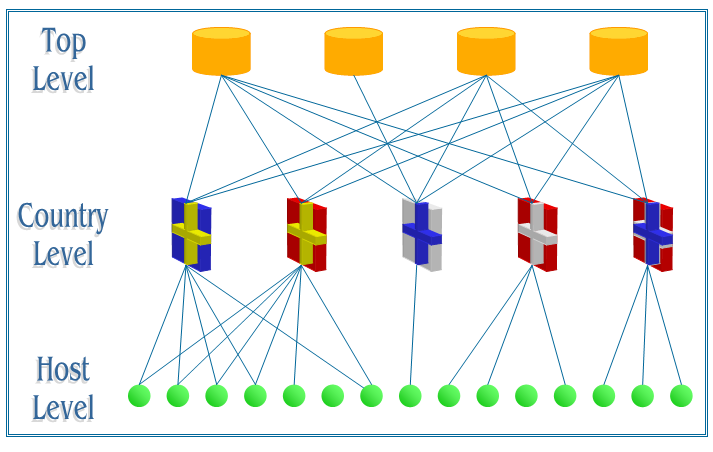
\includegraphics{tree_hierarchy.png}}}
}
\caption{\label{fig:index_tree} Resources (hosts) and Index Services are
linked via the registration process creating a multi-rooted tree topology}
\end{figure}


%TODO mention the possibility of alternative topologies, the extension of registration 
% process


\begin{table}
\centering
\begin{tabular}{|l|l|l|}
\hline
host &
port&
LDAP baseDN \\
\hline
\hline
index1.nordugrid.org &
2135 &
mds-vo-name=nordugrid,o=grid \\
\hline
index2.nordugrid.org &
2135 &
mds-vo-name=nordugrid,o=grid \\
\hline
index3.nordugrid.org &
2135 &
mds-vo-name=nordugrid,o=grid \\
\hline
index4.nordugrid.org &
2135 &
mds-vo-name=nordugrid,o=grid \\
\hline
\end{tabular}
\caption{\label{Table:topindices} LDAP URL of the TOP Level ARC Index Services}
\end{table}




\subsection{Resource discovery}

Resource discovery is the process when clients walk through the 
Index Services organized in a tree topology (see Fig.\ref{fig:index_tree})
and collect  LDAP contact URLs of the Computing and Storage resources.
The discovery process usually starts at the top of the tree by querying some of the 
Top Level Index Services(Table \ref{Table:topindices} lists the Top Indices). 
A Top Level Index Service is queried by a specially 
crafted ldapsearch (Figure \ref{fig:giisregistrationstatus}) which results 
all the registration entries stored in the Index Service. 
Index Services contain registration information of both resources and 
other Index Services. In the second step the client 
has to separate the entries corresponding to Index Services from entries
describing registrations of actual resources (Local Trees). 
The Figures\ref{fig:regentry1},\ref{fig:regentry2} show a registration table of
a Computing resource and an Index Service, respectively. 
The {\it Ldap-suffix} of a resource always contains the special string 
{\it "mds-vo-name=local,o=grid"} referring to the fact that the resource runs
a Local Information Tree. Then, the client contact the the newly discovered Index
Services and obtains the registration tables. The tables are separated into 
Indices and Resources, again. The process is repeated until all the Index Services 
are queried and the full list of LDAP Contact URL of Resources are collected. 

Once the client has collected a list of Resource LDAP Contact URLs 
from the Index Services,
the second phase of the information collection begins: 
The client directly contacts every Resource and initiates an LDAP query 
against the Local Information Tree.  
This is the real information gathering process in contrast to the first 
phase in which only the LDAP URLS were collected. Remember, 
unlike other systems (Globus GIIS, GT4 aggregator, R-GMA, LCG-BDII) 
ARC has no service  which caches or aggregates
Resource specific information on a higher level, 
ARC Index Services are not used to store local
information, Indices maintain only LDAP URLs.


\newpage
\appendix
\section{Clients of the ARC information system}


The entire content of the Information system including both the 
local trees and the Index Services are presented via an LDAP interface.
LDAP is a very well supported protocol, therefore it is very easy to 
construct clients making use of the ARC information system.

The Grid Monitor\cite{monitor} is a very powerful graphical interface 
to the Information System written in PHP. The monitor runs 
on a web-server and provides a browsable graphical representation of the 
information content of the Grid.

The matured command line client (UI)\cite{ui} or the 
Graphical UIs and  ARClib being developed  provide another examples
of straightforward interfaceability to the LDAP-based Information System.

%TODO ASK Oxana for the monitor - ldap attributes mapping
%reference to the ARCLIB/ new GUIS


\newpage

\section{LDAP Examples \label{appendix:examples}}


\begin{itemize}

\item
LDAP query against a local tree with a filter for nordugrid-cluster objectclass:

\tiny
\begin{verbatim}
ldapsearch -h bambi.hep.lu.se -p 2135 -x -b 'mds-vo-name=local,o=grid' 'objectclass=nordugrid-cluster'
version: 2

#
# filter: objectclass=nordugrid-cluster
# requesting: ALL
#

# bambi.hep.lu.se, local, grid
dn: nordugrid-cluster-name=bambi.hep.lu.se,Mds-Vo-name=local,o=grid
objectClass: Mds
objectClass: nordugrid-cluster
nordugrid-cluster-name: bambi.hep.lu.se
nordugrid-cluster-aliasname: Bambi Test Cluster
nordugrid-cluster-owner: EHEP
nordugrid-cluster-location: SE-221 00
nordugrid-cluster-issuerca: /O=Grid/O=NorduGrid/CN=NorduGrid Certification Aut
 hority
nordugrid-cluster-contactstring: gsiftp://bambi.hep.lu.se:2811/jobs
nordugrid-cluster-support: grid.support@mysite.org
nordugrid-cluster-support: grid.support@myproject.org
nordugrid-cluster-lrms-type: fork
nordugrid-cluster-lrms-config: single job per processor
nordugrid-cluster-architecture: i686
nordugrid-cluster-opsys: Mandrake-10.0
nordugrid-cluster-opsys: glibc-2.3.3-10mdk
nordugrid-cluster-benchmark: SPECINT2000 @ 222
nordugrid-cluster-benchmark: SPECFP2000 @ 333
nordugrid-cluster-homogeneity: True
nordugrid-cluster-nodecpu: Intel(R) Pentium(R) 4 CPU 3.00GHz @ 2993.100 MHz
nordugrid-cluster-nodeaccess: inbound
nordugrid-cluster-nodeaccess: outbound
nordugrid-cluster-totalcpus: 2
nordugrid-cluster-usedcpus: 0
nordugrid-cluster-cpudistribution: 2cpu:1
nordugrid-cluster-queuedjobs: 0
nordugrid-cluster-totaljobs: 0
nordugrid-cluster-sessiondir-free: 13958
nordugrid-cluster-sessiondir-total: 26403
nordugrid-cluster-cache-free: 9536
nordugrid-cluster-cache-total: 9536
nordugrid-cluster-middleware: nordugrid-0.5.20
nordugrid-cluster-middleware: globus-2.4.3-12ng
nordugrid-cluster-middleware: my grid software
nordugrid-cluster-runtimeenvironment: tt
Mds-validfrom: 20050307103026Z
Mds-validto: 20050307103029Z

# search result
search: 2
result: 0 Success

# numResponses: 2
# numEntries: 1
\end{verbatim}
\normalsize

\item Query for active Grid jobs stored in the local tree describing a computing resource:

\tiny
\begin{verbatim}
ldapsearch -h quark.hep.lu.se -p 2135 -x -b 'mds-vo-name=local,o=grid' 'objectclass=nordugrid-job'
version: 2

#
# filter: objectclass=nordugrid-job
# requesting: ALL
#

# gsiftp://quark.hep.lu.se:2811/jobs/131601109950874935622127, jobs, pc, quar
 k.hep.lu.se, local, grid
dn: nordugrid-job-globalid=gsiftp://quark.hep.lu.se:2811/jobs/1316011099508749
 35622127, nordugrid-info-group-name=jobs, nordugrid-queue-name=pc,nordugrid-c
 luster-name=quark.hep.lu.se,Mds-Vo-name=local,o=grid
objectClass: Mds
objectClass: nordugrid-job
nordugrid-job-globalid: gsiftp://quark.hep.lu.se:2811/jobs/1316011099508749356
 22127
nordugrid-job-globalowner: /O=Grid/O=NorduGrid/OU=cmm.ki.se/CN=Roxana Merino
nordugrid-job-jobname: TFBS2
nordugrid-job-submissiontime: 20050304154114Z
nordugrid-job-execcluster: quark.hep.lu.se
nordugrid-job-execqueue: pc
nordugrid-job-cpucount: 1
nordugrid-job-sessiondirerasetime: 20050305154232Z
nordugrid-job-stdout: tfbs.out
nordugrid-job-stderr: tfbs.out
nordugrid-job-gmlog: gmlog
nordugrid-job-runtimeenvironment: BIO-GEIJER-0.0.2
nordugrid-job-submissionui: 217.208.119.237:18236;10.0.0.1
nordugrid-job-clientsoftware: nordugrid-0.4.4
nordugrid-job-proxyexpirationtime: 20050304212024Z
nordugrid-job-status: DELETED
nordugrid-job-reqcputime: 2
nordugrid-job-executionnodes: node2
Mds-validfrom: 20050307110037Z
Mds-validto: 20050307110107Z

# gsiftp://quark.hep.lu.se:2811/jobs/5381111006551269125810, jobs, pclong, qu
 ark.hep.lu.se, local, grid
dn: nordugrid-job-globalid=gsiftp://quark.hep.lu.se:2811/jobs/5381111006551269
 125810, nordugrid-info-group-name=jobs, nordugrid-queue-name=pclong,nordugrid
 -cluster-name=quark.hep.lu.se,Mds-Vo-name=local,o=grid
objectClass: Mds
objectClass: nordugrid-job
nordugrid-job-globalid: gsiftp://quark.hep.lu.se:2811/jobs/5381111006551269125
 810
nordugrid-job-globalowner: /O=Grid/O=NorduGrid/OU=fys.ku.dk/CN=Brian Moller An
 dersen
nordugrid-job-jobname: selfconsistentMDSSAFNAF100slabonemu
nordugrid-job-submissiontime: 20050305233152Z
nordugrid-job-execcluster: quark.hep.lu.se
nordugrid-job-execqueue: pclong
nordugrid-job-cpucount: 1
nordugrid-job-stdout: output
nordugrid-job-stderr: output
nordugrid-job-submissionui: 130.225.102.149:33853;johansen.fys.ku.dk
nordugrid-job-clientsoftware: nordugrid-0.3.39
nordugrid-job-proxyexpirationtime: 20050306100826Z
nordugrid-job-status: INLRMS: R
nordugrid-job-usedmem: 30736
nordugrid-job-usedwalltime: 2127
nordugrid-job-usedcputime: 2125
nordugrid-job-reqcputime: 10080
nordugrid-job-executionnodes: node1/0
nordugrid-job-lrmscomment: Job started on Sun Mar 06 at 00:32
Mds-validfrom: 20050307110038Z
Mds-validto: 20050307110108Z

# gsiftp://quark.hep.lu.se:2811/jobs/52301110065467612188831, jobs, pclong, q
 uark.hep.lu.se, local, grid
dn: nordugrid-job-globalid=gsiftp://quark.hep.lu.se:2811/jobs/5230111006546761
 2188831, nordugrid-info-group-name=jobs, nordugrid-queue-name=pclong,nordugri
 d-cluster-name=quark.hep.lu.se,Mds-Vo-name=local,o=grid
objectClass: Mds
objectClass: nordugrid-job
nordugrid-job-globalid: gsiftp://quark.hep.lu.se:2811/jobs/5230111006546761218
 8831
nordugrid-job-globalowner: /O=Grid/O=NorduGrid/OU=fys.ku.dk/CN=Brian Moller An
 dersen
nordugrid-job-jobname: selfconsistentMDSSAFNAF100slabonemu
nordugrid-job-submissiontime: 20050305233107Z
nordugrid-job-execcluster: quark.hep.lu.se
nordugrid-job-execqueue: pclong
nordugrid-job-cpucount: 1
nordugrid-job-stdout: output
nordugrid-job-stderr: output
nordugrid-job-submissionui: 130.225.102.149:33846;johansen.fys.ku.dk
nordugrid-job-clientsoftware: nordugrid-0.3.39
nordugrid-job-proxyexpirationtime: 20050306100826Z
nordugrid-job-status: INLRMS: R
nordugrid-job-usedmem: 30736
nordugrid-job-usedwalltime: 2126
nordugrid-job-usedcputime: 2126
nordugrid-job-reqcputime: 10080
nordugrid-job-executionnodes: node3/0
nordugrid-job-lrmscomment: Job started on Sun Mar 06 at 00:32
Mds-validfrom: 20050307110038Z
Mds-validto: 20050307110108Z

# gsiftp://quark.hep.lu.se:2811/jobs/49831110065360908977417, jobs, pclong, q
 uark.hep.lu.se, local, grid
dn: nordugrid-job-globalid=gsiftp://quark.hep.lu.se:2811/jobs/4983111006536090
 8977417, nordugrid-info-group-name=jobs, nordugrid-queue-name=pclong,nordugri
 d-cluster-name=quark.hep.lu.se,Mds-Vo-name=local,o=grid
objectClass: Mds
objectClass: nordugrid-job
nordugrid-job-globalid: gsiftp://quark.hep.lu.se:2811/jobs/4983111006536090897
 7417
nordugrid-job-globalowner: /O=Grid/O=NorduGrid/OU=fys.ku.dk/CN=Brian Moller An
 dersen
nordugrid-job-jobname: selfconsistentMDSSAFNAF100slabonemu
nordugrid-job-submissiontime: 20050305232920Z
nordugrid-job-execcluster: quark.hep.lu.se
nordugrid-job-execqueue: pclong
nordugrid-job-cpucount: 1
nordugrid-job-stdout: output
nordugrid-job-stderr: output
nordugrid-job-submissionui: 130.225.102.149:33836;johansen.fys.ku.dk
nordugrid-job-clientsoftware: nordugrid-0.3.39
nordugrid-job-proxyexpirationtime: 20050306100826Z
nordugrid-job-status: INLRMS: R
nordugrid-job-usedmem: 30736
nordugrid-job-usedwalltime: 2128
nordugrid-job-usedcputime: 2128
nordugrid-job-reqcputime: 8640
nordugrid-job-executionnodes: node2/0
nordugrid-job-lrmscomment: Job started on Sun Mar 06 at 00:30
Mds-validfrom: 20050307110038Z
Mds-validto: 20050307110108Z

# search result
search: 2
result: 0 Success

# numResponses: 5
# numEntries: 4
\end{verbatim}
\normalsize


\item LDAP query to obtain the registration entries stored in an Index Service:

\tiny
\begin{verbatim}
ldapsearch -h quark.hep.lu.se -p 2135 -x -b 'mds-vo-name=Sweden,o=Grid' -s base giisregistrationstatus
version: 2

#
# filter: (objectclass=*)
# requesting: giisregistrationstatus
#

# se1:se1.hpc2n.umu.se, Sweden, grid
dn: nordugrid-se-name=se1:se1.hpc2n.umu.se, Mds-Vo-name=Sweden,o=grid
objectClass: Mds
objectClass: MdsVoOp
objectClass: MdsService
objectClass: MdsServiceLdap
Mds-Service-type: ldap
Mds-Service-hn: ido-i.hpc2n.umu.se
Mds-Service-port: 2135
Mds-Service-Ldap-suffix: nordugrid-se-name=se1:se1.hpc2n.umu.se, Mds-Vo-name=l
 ocal, o=grid
Mds-Service-Ldap-sizelimit: 0
Mds-Service-Ldap-timeout: 45
Mds-Service-Ldap-cachettl: 15
Mds-Bind-Method-servers: ANONYM-ONLY
Mds-Reg-status: VALID

# bphysics:quark.hep.lu.se, Sweden, grid
dn: nordugrid-se-name=bphysics:quark.hep.lu.se, Mds-Vo-name=Sweden,o=grid
objectClass: Mds
objectClass: MdsVoOp
objectClass: MdsService
objectClass: MdsServiceLdap
Mds-Service-type: ldap
Mds-Service-hn: quark.hep.lu.se
Mds-Service-port: 2135
Mds-Service-Ldap-suffix: nordugrid-se-name=bphysics:quark.hep.lu.se, Mds-Vo-na
 me=local, o=grid
Mds-Service-Ldap-sizelimit: 0
Mds-Service-Ldap-timeout: 45
Mds-Service-Ldap-cachettl: 15
Mds-Bind-Method-servers: ANONYM-ONLY
Mds-Reg-status: VALID

# Quark:quark.hep.lu.se, Sweden, grid
dn: nordugrid-se-name=Quark:quark.hep.lu.se, Mds-Vo-name=Sweden,o=grid
objectClass: Mds
objectClass: MdsVoOp
objectClass: MdsService
objectClass: MdsServiceLdap
Mds-Service-type: ldap
Mds-Service-hn: quark.hep.lu.se
Mds-Service-port: 2135
Mds-Service-Ldap-suffix: nordugrid-se-name=Quark:quark.hep.lu.se, Mds-Vo-name=
 local, o=grid
Mds-Service-Ldap-sizelimit: 0
Mds-Service-Ldap-timeout: 45
Mds-Service-Ldap-cachettl: 15
Mds-Bind-Method-servers: ANONYM-ONLY
Mds-Reg-status: PURGED

# quark.hep.lu.se, Sweden, grid
dn: nordugrid-cluster-name=quark.hep.lu.se, Mds-Vo-name=Sweden,o=grid
objectClass: Mds
objectClass: MdsVoOp
objectClass: MdsService
objectClass: MdsServiceLdap
Mds-Service-type: ldap
Mds-Service-hn: quark.hep.lu.se
Mds-Service-port: 2135
Mds-Service-Ldap-suffix: nordugrid-cluster-name=quark.hep.lu.se, Mds-Vo-name=l
 ocal, o=grid
Mds-Service-Ldap-sizelimit: 0
Mds-Service-Ldap-timeout: 45
Mds-Service-Ldap-cachettl: 0
Mds-Bind-Method-servers: ANONYM-ONLY
Mds-Reg-status: VALID

# files:grid.tsl.uu.se, Sweden, grid
dn: nordugrid-se-name=files:grid.tsl.uu.se, Mds-Vo-name=Sweden,o=grid
objectClass: Mds
objectClass: MdsVoOp
objectClass: MdsService
objectClass: MdsServiceLdap
Mds-Service-type: ldap
Mds-Service-hn: grid.tsl.uu.se
Mds-Service-port: 2135
Mds-Service-Ldap-suffix: nordugrid-se-name=files:grid.tsl.uu.se, Mds-Vo-name=l
 ocal, o=grid
Mds-Service-Ldap-sizelimit: 0
Mds-Service-Ldap-timeout: 45
Mds-Service-Ldap-cachettl: 15
Mds-Bind-Method-servers: ANONYM-ONLY
Mds-Reg-status: PURGED

# toto7.lunarc.lu.se, Sweden, grid
dn: nordugrid-cluster-name=toto7.lunarc.lu.se, Mds-Vo-name=Sweden,o=grid
objectClass: Mds
objectClass: MdsVoOp
objectClass: MdsService
objectClass: MdsServiceLdap
Mds-Service-type: ldap
Mds-Service-hn: toto7.lunarc.lu.se
Mds-Service-port: 2135
Mds-Service-Ldap-suffix: nordugrid-cluster-name=toto7.lunarc.lu.se, Mds-Vo-nam
 e=local, o=grid
Mds-Service-Ldap-sizelimit: 0
Mds-Service-Ldap-timeout: 45
Mds-Service-Ldap-cachettl: 0
Mds-Bind-Method-servers: ANONYM-ONLY
Mds-Reg-status: VALID

# Swegrid, Sweden, grid
dn: Mds-Vo-name=Swegrid, Mds-Vo-name=Sweden,o=grid
objectClass: Mds
objectClass: MdsVoOp
objectClass: MdsService
objectClass: MdsServiceLdap
Mds-Service-type: ldap
Mds-Service-hn: nexus.swegrid.se
Mds-Service-port: 2135
Mds-Service-Ldap-suffix: Mds-Vo-name=Swegrid, o=grid
Mds-Service-Ldap-sizelimit: 0
Mds-Service-Ldap-timeout: 120
Mds-Service-Ldap-cachettl: 30
Mds-Bind-Method-servers: ANONYM-ONLY
Mds-Reg-status: VALID

# search result
search: 2
result: 0 Success

# numResponses: 8
# numEntries: 7

\end{verbatim}
\normalsize

\end{itemize}


\newpage


\section{NorduGrid LDAP schema file\label{appendix:schema}}
\tiny

%
%TODO: Don't forget to insert the most recent schema file !!!!!!!!!
%
\begin{verbatim}

#---------------------------------------------------------
# These classes and attributes are imported from globus mds
# slightly to be proper LDAP schemas.

attributetype ( 1.3.6.1.4.1.11604.2.1.8.0.1
    NAME 'Mds-validfrom'
    DESC 'Object creation time'
    EQUALITY generalizedTimeMatch
    ORDERING generalizedTimeOrderingMatch
    SUBSTR caseIgnoreSubstringsMatch
    SYNTAX 1.3.6.1.4.1.1466.115.121.1.24
    SINGLE-VALUE
 )

attributetype ( 1.3.6.1.4.1.11604.2.1.8.0.2
    NAME 'Mds-validto'
    DESC 'Object expiration time'
    EQUALITY generalizedTimeMatch
    ORDERING generalizedTimeOrderingMatch
    SUBSTR caseIgnoreSubstringsMatch
    SYNTAX 1.3.6.1.4.1.1466.115.121.1.24
    SINGLE-VALUE
 )


attributetype ( 1.3.6.1.4.1.11604.2.1.8.0.3
    NAME 'Mds-keepto'
    DESC 'Object purge time'
    EQUALITY generalizedTimeMatch
    ORDERING generalizedTimeOrderingMatch
    SUBSTR caseIgnoreSubstringsMatch
    SYNTAX 1.3.6.1.4.1.1466.115.121.1.24
    SINGLE-VALUE
 )

objectclass ( 1.3.6.1.4.1.11604.2.1.8
    NAME 'Mds'
    ABSTRACT
    MUST ( Mds-validfrom $ Mds-validto )
    MAY Mds-keepto
 )

attributetype ( 1.3.6.1.4.1.11604.2.1.8.1.4.0.1
    NAME 'Mds-Vo-name'
    DESC 'Locally unique VO name'
    EQUALITY caseIgnoreMatch
    SYNTAX 1.3.6.1.4.1.1466.115.121.1.15
    SINGLE-VALUE
 )

objectclass ( 1.3.6.1.4.1.11604.2.1.8.1.4
    NAME 'MdsVo'
    SUP 'Mds'
    STRUCTURAL
    MUST Mds-Vo-name
 )

attributetype ( 1.3.6.1.4.1.11604.2.1.8.1.4.1.0.1
    NAME 'Mds-Vo-Op-name'
    DESC 'Locally unique Op name'
    EQUALITY caseIgnoreMatch
    ORDERING caseIgnoreOrderingMatch
    SUBSTR caseIgnoreSubstringsMatch
    SYNTAX 1.3.6.1.4.1.1466.115.121.1.44
    SINGLE-VALUE
 )

objectclass ( 1.3.6.1.4.1.11604.2.1.8.1.4.1
    NAME 'MdsVoOp'
    SUP 'Mds'
    STRUCTURAL
    MUST Mds-Vo-Op-name
 )

attributetype ( 1.3.6.1.4.1.11604.2.1.8.2.7.1.0.1
    NAME 'Mds-Service-type'
    DESC 'Service protocol'
    EQUALITY caseIgnoreMatch
    ORDERING caseIgnoreOrderingMatch
    SUBSTR caseIgnoreSubstringsMatch
    SYNTAX 1.3.6.1.4.1.1466.115.121.1.44
    SINGLE-VALUE
 )

attributetype ( 1.3.6.1.4.1.11604.2.1.8.2.7.1.0.2
    NAME 'Mds-Service-protocol'
    DESC 'Service protocol OID'
    EQUALITY caseIgnoreMatch
    ORDERING caseIgnoreOrderingMatch
    SUBSTR caseIgnoreSubstringsMatch
    SYNTAX 1.3.6.1.4.1.1466.115.121.1.44
 )

attributetype ( 1.3.6.1.4.1.11604.2.1.8.2.7.1.0.3
    NAME 'Mds-Service-port'
    DESC 'Service TCP port'
    EQUALITY integerMatch
    ORDERING integerOrderingMatch
    SUBSTR caseIgnoreSubstringsMatch
    SYNTAX 1.3.6.1.4.1.1466.115.121.1.27
    SINGLE-VALUE
 )

attributetype ( 1.3.6.1.4.1.11604.2.1.8.2.7.1.0.4
    NAME 'Mds-Service-hn'
    DESC 'Service FQDN hostname'
    EQUALITY caseIgnoreMatch
    ORDERING caseIgnoreOrderingMatch
    SUBSTR caseIgnoreSubstringsMatch
    SYNTAX 1.3.6.1.4.1.1466.115.121.1.44
    SINGLE-VALUE
 )

attributetype ( 1.3.6.1.4.1.11604.2.1.8.2.7.1.0.5
    NAME 'Mds-Service-url'
    DESC 'Service URL'
    EQUALITY caseIgnoreMatch
    ORDERING caseIgnoreOrderingMatch
    SUBSTR caseIgnoreSubstringsMatch
    SYNTAX 1.3.6.1.4.1.1466.115.121.1.44
    SINGLE-VALUE
 )

objectclass ( 1.3.6.1.4.1.11604.2.1.8.2.7.1
    NAME 'MdsService'
    SUP 'Mds'
    AUXILIARY
    MUST ( Mds-Service-type $ Mds-Service-protocol $ Mds-Service-port $ Mds-Service-hn )
    MAY Mds-Service-url
 )

attributetype ( 1.3.6.1.4.1.11604.2.1.8.2.7.1.1.0.1
    NAME 'Mds-Service-Ldap-suffix'
    DESC 'DN suffix of service'
    EQUALITY caseIgnoreMatch
    ORDERING caseIgnoreOrderingMatch
    SUBSTR caseIgnoreSubstringsMatch
    SYNTAX 1.3.6.1.4.1.1466.115.121.1.44
 )

attributetype ( 1.3.6.1.4.1.11604.2.1.8.2.7.1.1.0.2
    NAME 'Mds-Service-Ldap-timeout'
    DESC 'suggested timeout'
    EQUALITY caseIgnoreMatch
    ORDERING caseIgnoreOrderingMatch
    SUBSTR caseIgnoreSubstringsMatch
    SYNTAX 1.3.6.1.4.1.1466.115.121.1.44
 )

attributetype ( 1.3.6.1.4.1.11604.2.1.8.2.7.1.1.0.3
    NAME 'Mds-Service-Ldap-sizelimit'
    DESC 'suggested sizelimit'
    EQUALITY caseIgnoreMatch
    ORDERING caseIgnoreOrderingMatch
    SUBSTR caseIgnoreSubstringsMatch
    SYNTAX 1.3.6.1.4.1.1466.115.121.1.44
 )

attributetype ( 1.3.6.1.4.1.11604.2.1.8.2.7.1.1.0.4
    NAME 'Mds-Service-Ldap-cachettl'
    DESC 'suggested cacheability'
    EQUALITY caseIgnoreMatch
    ORDERING caseIgnoreOrderingMatch
    SUBSTR caseIgnoreSubstringsMatch
    SYNTAX 1.3.6.1.4.1.1466.115.121.1.44
 )

attributetype ( 1.3.6.1.4.1.11604.2.1.8.2.7.1.1.0.5
    NAME 'Mds-Service-Ldap-ttl'
    DESC 'suggested ttl'
    EQUALITY caseIgnoreMatch
    ORDERING caseIgnoreOrderingMatch
    SUBSTR caseIgnoreSubstringsMatch
    SYNTAX 1.3.6.1.4.1.1466.115.121.1.44
 )

attributetype ( 1.3.6.1.4.1.11604.2.1.8.2.7.1.1.0.10
    NAME 'Mds-Reg-status'
    DESC 'VALID/INVALID/PURGED'
    EQUALITY caseIgnoreMatch
    ORDERING caseIgnoreOrderingMatch
    SUBSTR caseIgnoreSubstringsMatch
    SYNTAX 1.3.6.1.4.1.1466.115.121.1.44
 )

attributetype ( 1.3.6.1.4.1.11604.2.1.8.2.7.1.1.0.11
    NAME 'Mds-Bind-Method-servers'
    DESC 'AUTHC-ONLY/AUTHC-FIRST/ANONYM-ONLY'
    EQUALITY caseIgnoreMatch
    ORDERING caseIgnoreOrderingMatch
    SUBSTR caseIgnoreSubstringsMatch
    SYNTAX 1.3.6.1.4.1.1466.115.121.1.44
 )

objectclass ( 1.3.6.1.4.1.11604.2.1.8.2.7.1.1
    NAME 'MdsServiceLdap'
    SUP 'MdsService'
    AUXILIARY
    MUST Mds-Service-Ldap-suffix
    MAY ( Mds-Service-Ldap-timeout $ Mds-Service-Ldap-sizelimit $ Mds-Service-Ldap-cachettl $ Mds-Service-Ldap-ttl $ Mds-Reg-status $ Mds-Bind-Method-servers )
 )

# attributes for the nordugrid-cluster objectclass 
#
attributetype ( 1.3.6.1.4.1.11604.2.1.1.1
    NAME 'nordugrid-cluster-name'
    DESC 'The name of the cluster specified as the domain name of the frontend'
    EQUALITY caseIgnoreMatch
    ORDERING caseIgnoreOrderingMatch
    SUBSTR caseIgnoreSubstringsMatch
    SYNTAX 1.3.6.1.4.1.1466.115.121.1.44
    SINGLE-VALUE )

attributetype ( 1.3.6.1.4.1.11604.2.1.1.2
    NAME 'nordugrid-cluster-aliasname'
    DESC 'The alias name of the cluster'
    EQUALITY caseIgnoreMatch
    ORDERING caseIgnoreOrderingMatch
    SUBSTR caseIgnoreSubstringsMatch
    SYNTAX 1.3.6.1.4.1.1466.115.121.1.15
    SINGLE-VALUE)
    
attributetype ( 1.3.6.1.4.1.11604.2.1.1.3
    NAME 'nordugrid-cluster-contactstring'
    DESC 'The URL of the job submission service running on the cluster frontend'
    EQUALITY caseExactIA5Match
    SUBSTR caseExactIA5SubstringsMatch
    SYNTAX 1.3.6.1.4.1.1466.115.121.1.26
    SINGLE-VALUE )
    
attributetype ( 1.3.6.1.4.1.11604.2.1.1.4
    NAME 'nordugrid-cluster-support'
    DESC 'RFC822 email address of support'
    EQUALITY caseIgnoreIA5Match
    SYNTAX 1.3.6.1.4.1.1466.115.121.1.26{256})

attributetype ( 1.3.6.1.4.1.11604.2.1.1.5
    NAME 'nordugrid-cluster-lrms-type'
    DESC 'The type of the Local Resource Management System'
    EQUALITY caseIgnoreMatch
    ORDERING caseIgnoreOrderingMatch
    SUBSTR caseIgnoreSubstringsMatch
    SYNTAX 1.3.6.1.4.1.1466.115.121.1.44
    SINGLE-VALUE )
    
attributetype ( 1.3.6.1.4.1.11604.2.1.1.6
    NAME 'nordugrid-cluster-lrms-version'
    DESC 'The version of the Local Resource Management System'
    EQUALITY caseIgnoreMatch
    ORDERING caseIgnoreOrderingMatch
    SUBSTR caseIgnoreSubstringsMatch
    SYNTAX 1.3.6.1.4.1.1466.115.121.1.15
    SINGLE-VALUE )

attributetype ( 1.3.6.1.4.1.11604.2.1.1.7
    NAME 'nordugrid-cluster-lrms-config'
    DESC 'Additional remark on the LRMS config'
    EQUALITY caseIgnoreMatch
    ORDERING caseIgnoreOrderingMatch
    SUBSTR caseIgnoreSubstringsMatch
    SYNTAX 1.3.6.1.4.1.1466.115.121.1.15
    SINGLE-VALUE )

attributetype ( 1.3.6.1.4.1.11604.2.1.1.8
    NAME 'nordugrid-cluster-architecture'
    DESC 'The architecture of the cluster nodes'
    EQUALITY caseIgnoreMatch
    ORDERING caseIgnoreOrderingMatch
    SUBSTR caseIgnoreSubstringsMatch
    SYNTAX 1.3.6.1.4.1.1466.115.121.1.15
    SINGLE-VALUE )

attributetype ( 1.3.6.1.4.1.11604.2.1.1.9
    NAME 'nordugrid-cluster-opsys'
    DESC 'The operating system of the machines of the cluster'
    EQUALITY caseIgnoreMatch
    ORDERING caseIgnoreOrderingMatch
    SUBSTR caseIgnoreSubstringsMatch
    SYNTAX 1.3.6.1.4.1.1466.115.121.1.15)
  
attributetype ( 1.3.6.1.4.1.11604.2.1.1.10
    NAME 'nordugrid-cluster-homogeneity'
    DESC 'A logical flag indicating the homogeneity of the cluster nodes'
    EQUALITY booleanMatch
    SYNTAX 1.3.6.1.4.1.1466.115.121.1.7
    SINGLE-VALUE )   

attributetype ( 1.3.6.1.4.1.11604.2.1.1.11
    NAME 'nordugrid-cluster-nodecpu'
    DESC 'The cpu type of the nodes expressed in a fixed form (model name + MHz)'
    EQUALITY caseIgnoreMatch
    SYNTAX 1.3.6.1.4.1.1466.115.121.1.15
    SINGLE-VALUE )

attributetype ( 1.3.6.1.4.1.11604.2.1.1.12
    NAME 'nordugrid-cluster-nodememory'
    DESC 'The amount of memory which can be guaranteed to be available on the node in MB'
    EQUALITY integerMatch
    ORDERING integerOrderingMatch
    SUBSTR caseIgnoreSubstringsMatch
    SYNTAX 1.3.6.1.4.1.1466.115.121.1.27
    SINGLE-VALUE )

attributetype ( 1.3.6.1.4.1.11604.2.1.1.13
    NAME 'nordugrid-cluster-totalcpus'
    DESC 'The total number of cpus in the cluster'
    EQUALITY integerMatch
    ORDERING integerOrderingMatch
    SUBSTR caseIgnoreSubstringsMatch
    SYNTAX 1.3.6.1.4.1.1466.115.121.1.27
    SINGLE-VALUE ) 

attributetype ( 1.3.6.1.4.1.11604.2.1.1.14
    NAME 'nordugrid-cluster-cpudistribution'
    DESC 'The cpu distribution of the nodes given in the form of 1cpu:3 2cpu:4 4cpu:1'
    EQUALITY caseIgnoreMatch
    ORDERING caseIgnoreOrderingMatch
    SUBSTR caseIgnoreSubstringsMatch
    SYNTAX 1.3.6.1.4.1.1466.115.121.1.44
    SINGLE-VALUE )
    
attributetype ( 1.3.6.1.4.1.11604.2.1.1.15
    NAME 'nordugrid-cluster-sessiondir-free'
    DESC 'Free diskspace in MB of the sessiondirectory on the cluster'
    EQUALITY integerMatch
    ORDERING integerOrderingMatch
    SUBSTR caseIgnoreSubstringsMatch
    SYNTAX 1.3.6.1.4.1.1466.115.121.1.27
    SINGLE-VALUE )
    
attributetype ( 1.3.6.1.4.1.11604.2.1.1.16
    NAME 'nordugrid-cluster-sessiondir-total'
    DESC 'Total diskspace in MB of the sessiondirectory on the cluster'
    EQUALITY integerMatch
    ORDERING integerOrderingMatch
    SUBSTR caseIgnoreSubstringsMatch
    SYNTAX 1.3.6.1.4.1.1466.115.121.1.27
    SINGLE-VALUE )

attributetype ( 1.3.6.1.4.1.11604.2.1.1.17
    NAME 'nordugrid-cluster-cache-free'
    DESC 'Free diskspace in MB of the cache area on the cluster'
    EQUALITY integerMatch
    ORDERING integerOrderingMatch
    SUBSTR caseIgnoreSubstringsMatch
    SYNTAX 1.3.6.1.4.1.1466.115.121.1.27
    SINGLE-VALUE )
    
attributetype ( 1.3.6.1.4.1.11604.2.1.1.18
    NAME 'nordugrid-cluster-cache-total'
    DESC 'Total diskspace in MB of the cache area on the cluster'
    EQUALITY integerMatch
    ORDERING integerOrderingMatch
    SUBSTR caseIgnoreSubstringsMatch
    SYNTAX 1.3.6.1.4.1.1466.115.121.1.27
    SINGLE-VALUE )

attributetype ( 1.3.6.1.4.1.11604.2.1.1.19
    NAME 'nordugrid-cluster-runtimeenvironment'
    DESC 'preinstalled software packages of the cluster'
    EQUALITY caseIgnoreMatch
    ORDERING caseIgnoreOrderingMatch
    SUBSTR caseIgnoreSubstringsMatch
    SYNTAX 1.3.6.1.4.1.1466.115.121.1.15 )

attributetype ( 1.3.6.1.4.1.11604.2.1.1.20
    NAME 'nordugrid-cluster-localse'
    DESC 'The URL of a storage element considered to be local to the cluster'
    EQUALITY caseExactMatch
    ORDERING caseExactOrderingMatch
    SUBSTR caseExactSubstringsMatch
    SYNTAX 1.3.6.1.4.1.1466.115.121.1.15 )  

attributetype ( 1.3.6.1.4.1.11604.2.1.1.21
    NAME 'nordugrid-cluster-middleware'
    DESC 'The middleware packages on the cluster'
    EQUALITY caseIgnoreMatch
    ORDERING caseIgnoreOrderingMatch
    SUBSTR caseIgnoreSubstringsMatch
    SYNTAX 1.3.6.1.4.1.1466.115.121.1.15 )
    
attributetype ( 1.3.6.1.4.1.11604.2.1.1.22
    NAME 'nordugrid-cluster-totaljobs'
    DESC 'The total number of jobs (Grid + non-Grid) in the cluster'
    EQUALITY integerMatch
    ORDERING integerOrderingMatch
    SUBSTR caseIgnoreSubstringsMatch
    SYNTAX 1.3.6.1.4.1.1466.115.121.1.27
    SINGLE-VALUE ) 
       
attributetype ( 1.3.6.1.4.1.11604.2.1.1.23
    NAME 'nordugrid-cluster-usedcpus'
    DESC 'The total number of occupied cpus in the cluster'
    EQUALITY integerMatch
    ORDERING integerOrderingMatch
    SUBSTR caseIgnoreSubstringsMatch
    SYNTAX 1.3.6.1.4.1.1466.115.121.1.27
    SINGLE-VALUE )  
    
attributetype ( 1.3.6.1.4.1.11604.2.1.1.24
    NAME 'nordugrid-cluster-queuedjobs'
    DESC 'The total number of jobs (grid and non-grid) not-yet running: preparing or waiting to run 
          on the cluster, either in the grid-manager or in the LRMS. 
	  The attribute is TO BE DEPRECATED'
    EQUALITY integerMatch
    ORDERING integerOrderingMatch
    SUBSTR caseIgnoreSubstringsMatch
    SYNTAX 1.3.6.1.4.1.1466.115.121.1.27
    SINGLE-VALUE )   

attributetype ( 1.3.6.1.4.1.11604.2.1.1.25
    NAME 'nordugrid-cluster-location'
    DESC 'The geographical location of the cluster expressed in terms of a Postal ZIP code'
    EQUALITY caseIgnoreMatch
    ORDERING caseIgnoreOrderingMatch
    SUBSTR caseIgnoreSubstringsMatch
    SYNTAX 1.3.6.1.4.1.1466.115.121.1.44 
    SINGLE-VALUE )
    
attributetype ( 1.3.6.1.4.1.11604.2.1.1.26
    NAME 'nordugrid-cluster-owner'
    DESC 'The owner of the resource'
    EQUALITY caseIgnoreMatch
    ORDERING caseIgnoreOrderingMatch
    SUBSTR caseIgnoreSubstringsMatch
    SYNTAX 1.3.6.1.4.1.1466.115.121.1.15 ) 
        
attributetype ( 1.3.6.1.4.1.11604.2.1.1.27
    NAME 'nordugrid-cluster-issuerca'
    DESC 'The DN of the Certificate Authority which issued the certificate of the cluster'
    EQUALITY caseIgnoreMatch
    ORDERING caseIgnoreOrderingMatch
    SUBSTR caseIgnoreSubstringsMatch
    SYNTAX 1.3.6.1.4.1.1466.115.121.1.15 
    SINGLE-VALUE ) 

attributetype ( 1.3.6.1.4.1.11604.2.1.1.28
    NAME 'nordugrid-cluster-nodeaccess'
    DESC 'The inbound/outbound network accessibility of the nodes'
    EQUALITY caseIgnoreMatch
    ORDERING caseIgnoreOrderingMatch
    SUBSTR caseIgnoreSubstringsMatch
    SYNTAX 1.3.6.1.4.1.1466.115.121.1.44 )
    
attributetype ( 1.3.6.1.4.1.11604.2.1.1.29
    NAME 'nordugrid-cluster-comment'
    DESC 'Free form comment'
    EQUALITY caseIgnoreMatch
    ORDERING caseIgnoreOrderingMatch
    SUBSTR caseIgnoreSubstringsMatch
    SYNTAX 1.3.6.1.4.1.1466.115.121.1.15
    SINGLE-VALUE )    
 
attributetype ( 1.3.6.1.4.1.11604.2.1.1.30
    NAME 'nordugrid-cluster-interactive-contactstring'
    DESC 'The URL for interactive login'
    EQUALITY caseExactIA5Match
    SUBSTR caseExactIA5SubstringsMatch
    SYNTAX 1.3.6.1.4.1.1466.115.121.1.26 ) 

attributetype ( 1.3.6.1.4.1.11604.2.1.1.31
    NAME 'nordugrid-cluster-benchmark'
    DESC '@ separated benchmark_name, benchmark_value pair characterizing the cluster nodes'
    EQUALITY caseIgnoreMatch
    ORDERING caseIgnoreOrderingMatch
    SUBSTR caseIgnoreSubstringsMatch
    SYNTAX 1.3.6.1.4.1.1466.115.121.1.15 ) 

attributetype ( 1.3.6.1.4.1.11604.2.1.1.32
    NAME 'nordugrid-cluster-sessiondir-lifetime'
    DESC 'The lifetime of the sessiondir after the job has completed (in minutes)'
    EQUALITY integerMatch
    ORDERING integerOrderingMatch
    SUBSTR caseIgnoreSubstringsMatch
    SYNTAX 1.3.6.1.4.1.1466.115.121.1.27
    SINGLE-VALUE )

attributetype ( 1.3.6.1.4.1.11604.2.1.1.33
    NAME 'nordugrid-cluster-prelrmsqueued'
    DESC 'The total number of grid jobs not-yet reached the LRMS: preparing or queuing in the grid-layer'
    EQUALITY integerMatch
    ORDERING integerOrderingMatch
    SUBSTR caseIgnoreSubstringsMatch
    SYNTAX 1.3.6.1.4.1.1466.115.121.1.27
    SINGLE-VALUE )   

attributetype ( 1.3.6.1.4.1.11604.2.1.1.34
    NAME 'nordugrid-cluster-issuerca-hash'
    DESC 'The HASH of the Certificate Authority which issued the certificate for the cluster'
    EQUALITY caseExactMatch
    ORDERING caseExactOrderingMatch
    SUBSTR caseExactSubstringsMatch
    SYNTAX 1.3.6.1.4.1.1466.115.121.1.44 
    SINGLE-VALUE )  

attributetype ( 1.3.6.1.4.1.11604.2.1.1.35
    NAME 'nordugrid-cluster-trustedca'
    DESC 'The DN of a Certificate Authority trusted by the cluster'
    EQUALITY caseIgnoreMatch
    SYNTAX 1.3.6.1.4.1.1466.115.121.1.15 )

attributetype ( 1.3.6.1.4.1.11604.2.1.1.36
    NAME 'nordugrid-cluster-acl'
    DESC 'Cluster authorization information'
    EQUALITY caseExactMatch
    ORDERING caseExactOrderingMatch
    SUBSTR caseExactSubstringsMatch
    SYNTAX 1.3.6.1.4.1.1466.115.121.1.44 )

attributetype (1.3.6.1.4.1.11604.2.1.1.37
    NAME 'nordugrid-cluster-credentialexpirationtime'
    DESC 'The expiration date of the shortest living credential affecting the cluster's x509 environment in GMT'
    EQUALITY generalizedTimeMatch
    ORDERING generalizedTimeOrderingMatch
    SUBSTR caseIgnoreSubstringsMatch
    SYNTAX 1.3.6.1.4.1.1466.115.121.1.24
    SINGLE-VALUE )

objectclass ( 1.3.6.1.4.1.11604.2.1.1
    NAME 'nordugrid-cluster'
    DESC 'Description of a Nordugrid cluster'
    SUP 'Mds'
    STRUCTURAL
    MUST ( nordugrid-cluster-name $ nordugrid-cluster-contactstring )
    MAY  ( nordugrid-cluster-aliasname $ nordugrid-cluster-support $
           nordugrid-cluster-lrms-type $ nordugrid-cluster-lrms-version $
	   nordugrid-cluster-lrms-config $ nordugrid-cluster-architecture $
	   nordugrid-cluster-opsys $ nordugrid-cluster-homogeneity $
	   nordugrid-cluster-nodecpu $ nordugrid-cluster-nodememory $
	   nordugrid-cluster-totalcpus $ nordugrid-cluster-cpudistribution $
	   nordugrid-cluster-sessiondir-free $ nordugrid-cluster-sessiondir-total $
	   nordugrid-cluster-cache-free $ nordugrid-cluster-cache-total $
	   nordugrid-cluster-runtimeenvironment $ nordugrid-cluster-localse $
	   nordugrid-cluster-middleware $ nordugrid-cluster-totaljobs $
	   nordugrid-cluster-usedcpus $	nordugrid-cluster-queuedjobs  $
	   nordugrid-cluster-location $ nordugrid-cluster-owner $ 
	   nordugrid-cluster-issuerca $ nordugrid-cluster-nodeaccess $
	   nordugrid-cluster-comment $ nordugrid-cluster-interactive-contactstring $
	   nordugrid-cluster-benchmark $ nordugrid-cluster-sessiondir-lifetime $
	   nordugrid-cluster-prelrmsqueued $ nordugrid-cluster-issuerca-hash $
	   nordugrid-cluster-trustedca $ nordugrid-cluster-acl $
	   nordugrid-cluster-credentialexpirationtime ))

#-----------------------------------------------------------------
# attributes for the nordugrid-info-group objectclass
#
attributetype ( 1.3.6.1.4.1.11604.2.1.2.1
    NAME 'nordugrid-info-group-name'
    DESC 'Locally unique info group name'
    EQUALITY caseIgnoreMatch
    ORDERING caseIgnoreOrderingMatch
    SUBSTR caseIgnoreSubstringsMatch
    SYNTAX 1.3.6.1.4.1.1466.115.121.1.44
    SINGLE-VALUE)
    
objectclass ( 1.3.6.1.4.1.11604.2.1.2
    NAME 'nordugrid-info-group'
    DESC 'A general entry for grouping together MDS entries'
    SUP 'Mds'
    STRUCTURAL
    MUST ( nordugrid-info-group-name ))

#-----------------------------------------------------------------
# attributes for the nordugrid-queue objectclass
#
attributetype ( 1.3.6.1.4.1.11604.2.1.3.1
    NAME 'nordugrid-queue-name'
    DESC 'The queue name'
    EQUALITY caseExactMatch
    ORDERING caseExactOrderingMatch
    SUBSTR caseExactSubstringsMatch
    SYNTAX 1.3.6.1.4.1.1466.115.121.1.44
    SINGLE-VALUE )

attributetype ( 1.3.6.1.4.1.11604.2.1.3.2
    NAME 'nordugrid-queue-status'
    DESC 'The queue status'
    EQUALITY caseIgnoreMatch
    ORDERING caseIgnoreOrderingMatch
    SUBSTR caseIgnoreSubstringsMatch
    SYNTAX 1.3.6.1.4.1.1466.115.121.1.44
    SINGLE-VALUE )

attributetype ( 1.3.6.1.4.1.11604.2.1.3.3
    NAME 'nordugrid-queue-running'
    DESC 'Number of running jobs (Grid + non-Grid) in the queue with multi-node jobs multiciplity'
    EQUALITY integerMatch
    ORDERING integerOrderingMatch
    SUBSTR caseIgnoreSubstringsMatch
    SYNTAX 1.3.6.1.4.1.1466.115.121.1.27
    SINGLE-VALUE )

attributetype ( 1.3.6.1.4.1.11604.2.1.3.4
    NAME 'nordugrid-queue-queued'
    DESC 'The number of jobs (Grid + non-Grid) waiting in the queue.
          The attribute is TO BE DEPRECATED'
    EQUALITY integerMatch
    ORDERING integerOrderingMatch
    SUBSTR caseIgnoreSubstringsMatch
    SYNTAX 1.3.6.1.4.1.1466.115.121.1.27
    SINGLE-VALUE )

attributetype ( 1.3.6.1.4.1.11604.2.1.3.5
    NAME 'nordugrid-queue-maxrunning'
    DESC 'The maximum number of jobs allowed to run from this queue'
    EQUALITY integerMatch
    ORDERING integerOrderingMatch
    SUBSTR caseIgnoreSubstringsMatch
    SYNTAX 1.3.6.1.4.1.1466.115.121.1.27
    SINGLE-VALUE )

attributetype ( 1.3.6.1.4.1.11604.2.1.3.6
    NAME 'nordugrid-queue-maxqueuable'
    DESC 'The maximum number of jobs allowed to reside in the queue'
    EQUALITY integerMatch
    ORDERING integerOrderingMatch
    SUBSTR caseIgnoreSubstringsMatch
    SYNTAX 1.3.6.1.4.1.1466.115.121.1.27
    SINGLE-VALUE )

attributetype ( 1.3.6.1.4.1.11604.2.1.3.7
    NAME 'nordugrid-queue-maxuserrun'
    DESC 'Maximum number of jobs a user can run at the same time'
    EQUALITY integerMatch
    ORDERING integerOrderingMatch
    SUBSTR caseIgnoreSubstringsMatch
    SYNTAX 1.3.6.1.4.1.1466.115.121.1.27
    SINGLE-VALUE )

attributetype ( 1.3.6.1.4.1.11604.2.1.3.8
    NAME 'nordugrid-queue-maxcputime'
    DESC 'The maximum cputime allowed in this queue (in minutes)'
    EQUALITY integerMatch
    ORDERING integerOrderingMatch
    SUBSTR caseIgnoreSubstringsMatch
    SYNTAX 1.3.6.1.4.1.1466.115.121.1.27
    SINGLE-VALUE )

attributetype ( 1.3.6.1.4.1.11604.2.1.3.9
    NAME 'nordugrid-queue-mincputime'
    DESC 'The minimum possible cputime of this queue (in minutes)'
    EQUALITY integerMatch
    ORDERING integerOrderingMatch
    SUBSTR caseIgnoreSubstringsMatch
    SYNTAX 1.3.6.1.4.1.1466.115.121.1.27
    SINGLE-VALUE )

attributetype ( 1.3.6.1.4.1.11604.2.1.3.10
    NAME 'nordugrid-queue-defaultcputime'
    DESC 'The default cputime assigned to this queue (in minutes)'
    EQUALITY integerMatch
    ORDERING integerOrderingMatch
    SUBSTR caseIgnoreSubstringsMatch
    SYNTAX 1.3.6.1.4.1.1466.115.121.1.27
    SINGLE-VALUE )

attributetype ( 1.3.6.1.4.1.11604.2.1.3.11
    NAME 'nordugrid-queue-schedulingpolicy'
    DESC 'The scheduling policy of the queue (i.e. FIFO)'
    EQUALITY caseIgnoreMatch
    ORDERING caseIgnoreOrderingMatch
    SUBSTR caseIgnoreSubstringsMatch
    SYNTAX 1.3.6.1.4.1.1466.115.121.1.44
    SINGLE-VALUE )

attributetype ( 1.3.6.1.4.1.11604.2.1.3.12
    NAME 'nordugrid-queue-totalcpus'
    DESC 'Total number of cpus assigned to the queue'
    EQUALITY integerMatch
    ORDERING integerOrderingMatch
    SUBSTR caseIgnoreSubstringsMatch
    SYNTAX 1.3.6.1.4.1.1466.115.121.1.27
    SINGLE-VALUE )

attributetype ( 1.3.6.1.4.1.11604.2.1.3.13
    NAME 'nordugrid-queue-nodecpu'
    DESC 'The cpu type of the nodes assigned to the queue (model name + MHz)'
    EQUALITY caseIgnoreMatch
    SYNTAX 1.3.6.1.4.1.1466.115.121.1.15
    SINGLE-VALUE )

attributetype ( 1.3.6.1.4.1.11604.2.1.3.14
    NAME 'nordugrid-queue-nodememory'
    DESC 'The installed memory of a node assigned to the queue in MB'
    EQUALITY integerMatch
    ORDERING integerOrderingMatch
    SUBSTR caseIgnoreSubstringsMatch
    SYNTAX 1.3.6.1.4.1.1466.115.121.1.27
    SINGLE-VALUE )

attributetype ( 1.3.6.1.4.1.11604.2.1.3.15
    NAME 'nordugrid-queue-architecture'
    DESC 'The architecture of the machines in the queue'
    EQUALITY caseIgnoreMatch
    ORDERING caseIgnoreOrderingMatch
    SUBSTR caseIgnoreSubstringsMatch
    SYNTAX 1.3.6.1.4.1.1466.115.121.1.15
    SINGLE-VALUE )
    
attributetype ( 1.3.6.1.4.1.11604.2.1.3.16
    NAME 'nordugrid-queue-opsys'
    DESC 'The operating system of the nodes in the queue'
    EQUALITY caseIgnoreMatch
    ORDERING caseIgnoreOrderingMatch
    SUBSTR caseIgnoreSubstringsMatch
    SYNTAX 1.3.6.1.4.1.1466.115.121.1.15)
        
attributetype ( 1.3.6.1.4.1.11604.2.1.3.17
    NAME 'nordugrid-queue-gridrunning'
    DESC 'Number of running Grid jobs in the queue with multi-node jobs multiciplity'
    EQUALITY integerMatch
    ORDERING integerOrderingMatch
    SUBSTR caseIgnoreSubstringsMatch
    SYNTAX 1.3.6.1.4.1.1466.115.121.1.27
    SINGLE-VALUE )

attributetype ( 1.3.6.1.4.1.11604.2.1.3.18
    NAME 'nordugrid-queue-gridqueued'
    DESC 'The number of Grid jobs waiting in the LRMS queue'
    EQUALITY integerMatch
    ORDERING integerOrderingMatch
    SUBSTR caseIgnoreSubstringsMatch
    SYNTAX 1.3.6.1.4.1.1466.115.121.1.27
    SINGLE-VALUE )

attributetype ( 1.3.6.1.4.1.11604.2.1.3.19
    NAME 'nordugrid-queue-comment'
    DESC 'Free form comment'
    EQUALITY caseIgnoreMatch
    ORDERING caseIgnoreOrderingMatch
    SUBSTR caseIgnoreSubstringsMatch
    SYNTAX 1.3.6.1.4.1.1466.115.121.1.15
    SINGLE-VALUE )    

attributetype ( 1.3.6.1.4.1.11604.2.1.3.20
    NAME 'nordugrid-queue-benchmark'
    DESC 'Colon separated benchmark_name, benchmark_value pair characterizing the queue'
    EQUALITY caseIgnoreMatch
    ORDERING caseIgnoreOrderingMatch
    SUBSTR caseIgnoreSubstringsMatch
    SYNTAX 1.3.6.1.4.1.1466.115.121.1.15 ) 
 
attributetype ( 1.3.6.1.4.1.11604.2.1.3.21
    NAME 'nordugrid-queue-homogeneity'
    DESC 'A logical flag indicating the homogeneity of the queue nodes'
    EQUALITY booleanMatch  
    SYNTAX 1.3.6.1.4.1.1466.115.121.1.7
    SINGLE-VALUE ) 

attributetype ( 1.3.6.1.4.1.11604.2.1.3.22
    NAME 'nordugrid-queue-prelrmsqueued'
    DESC 'The number of Grid jobs belonging to this queue being processed
    	 or waiting in the Grid-layer before the LRMS submission.'      
    EQUALITY integerMatch
    ORDERING integerOrderingMatch
    SUBSTR caseIgnoreSubstringsMatch
    SYNTAX 1.3.6.1.4.1.1466.115.121.1.27
    SINGLE-VALUE )

attributetype ( 1.3.6.1.4.1.11604.2.1.3.23
    NAME 'nordugrid-queue-localqueued'
    DESC 'The number of non-Grid jobs waiting in the LRMS queue.'    
    EQUALITY integerMatch
    ORDERING integerOrderingMatch
    SUBSTR caseIgnoreSubstringsMatch
    SYNTAX 1.3.6.1.4.1.1466.115.121.1.27
    SINGLE-VALUE )
    
attributetype ( 1.3.6.1.4.1.11604.2.1.3.24
    NAME 'nordugrid-queue-maxwalltime'
    DESC 'The maximum walltime allowed in this queue (in minutes)'
    EQUALITY integerMatch
    ORDERING integerOrderingMatch
    SUBSTR caseIgnoreSubstringsMatch
    SYNTAX 1.3.6.1.4.1.1466.115.121.1.27
    SINGLE-VALUE )

attributetype ( 1.3.6.1.4.1.11604.2.1.3.25
    NAME 'nordugrid-queue-minwalltime'
    DESC 'The minimum possible walltime of this queue (in minutes)'
    EQUALITY integerMatch
    ORDERING integerOrderingMatch
    SUBSTR caseIgnoreSubstringsMatch
    SYNTAX 1.3.6.1.4.1.1466.115.121.1.27
    SINGLE-VALUE )

attributetype ( 1.3.6.1.4.1.11604.2.1.3.26
    NAME 'nordugrid-queue-defaultwalltime'
    DESC 'The default walltime assigned to this queue (in minutes)'
    EQUALITY integerMatch
    ORDERING integerOrderingMatch
    SUBSTR caseIgnoreSubstringsMatch
    SYNTAX 1.3.6.1.4.1.1466.115.121.1.27
    SINGLE-VALUE )     

attributetype ( 1.3.6.1.4.1.11604.2.1.3.27
    NAME 'nordugrid-queue-maxtotalcputime'
    DESC 'The maximum total cputime allowed in this queue (in minutes)'
    EQUALITY integerMatch
    ORDERING integerOrderingMatch
    SUBSTR caseIgnoreSubstringsMatch
    SYNTAX 1.3.6.1.4.1.1466.115.121.1.27
    SINGLE-VALUE )

objectclass ( 1.3.6.1.4.1.11604.2.1.3
    NAME 'nordugrid-queue'
    DESC 'An LRMS queue'
    SUP 'Mds'
    STRUCTURAL
    MUST ( nordugrid-queue-name $ nordugrid-queue-status)    
    MAY  ( nordugrid-queue-running $ nordugrid-queue-queued $
    	   nordugrid-queue-maxrunning  $ nordugrid-queue-maxqueuable$
    	   nordugrid-queue-maxuserrun $ nordugrid-queue-maxcputime $
    	   nordugrid-queue-mincputime $ nordugrid-queue-defaultcputime $
    	   nordugrid-queue-schedulingpolicy $ nordugrid-queue-totalcpus $
    	   nordugrid-queue-nodecpu $ nordugrid-queue-nodememory $
	   nordugrid-queue-opsys $ nordugrid-queue-architecture $	   
	   nordugrid-queue-gridrunning $ nordugrid-queue-gridqueued $
	   nordugrid-queue-comment $ nordugrid-queue-benchmark $
	   nordugrid-queue-homogeneity $ nordugrid-queue-prelrmsqueued $
	   nordugrid-queue-localqueued $ nordugrid-queue-maxwalltime $
	   nordugrid-queue-minwalltime $ nordugrid-queue-defaultwalltime $
	   nordugrid-queue-maxtotalcputime ))

#-----------------------------------------------------------------
#attributes for the nordugrid-job objectclass
#
attributetype ( 1.3.6.1.4.1.11604.2.1.4.1
    NAME 'nordugrid-job-globalid'
    DESC 'The global job identifier string'
    EQUALITY caseExactIA5Match
    SUBSTR caseExactIA5SubstringsMatch
    SYNTAX 1.3.6.1.4.1.1466.115.121.1.26    
    SINGLE-VALUE )

attributetype ( 1.3.6.1.4.1.11604.2.1.4.2
    NAME 'nordugrid-job-globalowner'
    DESC 'The SubjectName of the job owner'
    EQUALITY caseExactMatch
    ORDERING caseExactOrderingMatch
    SUBSTR caseExactSubstringsMatch
    SYNTAX 1.3.6.1.4.1.1466.115.121.1.44  
    SINGLE-VALUE )

attributetype ( 1.3.6.1.4.1.11604.2.1.4.3
    NAME 'nordugrid-job-execcluster'
    DESC 'The name of the execution cluster'
    EQUALITY caseIgnoreMatch
    ORDERING caseIgnoreOrderingMatch
    SUBSTR caseIgnoreSubstringsMatch
    SYNTAX 1.3.6.1.4.1.1466.115.121.1.15
    SINGLE-VALUE)

attributetype ( 1.3.6.1.4.1.11604.2.1.4.4
    NAME 'nordugrid-job-execqueue'
    DESC 'The name of the execution queue'
    EQUALITY caseIgnoreMatch
    ORDERING caseIgnoreOrderingMatch
    SUBSTR caseIgnoreSubstringsMatch
    SYNTAX 1.3.6.1.4.1.1466.115.121.1.44
    SINGLE-VALUE )
    
attributetype ( 1.3.6.1.4.1.11604.2.1.4.5
    NAME 'nordugrid-job-stdout'
    DESC 'The name of the file which contains the stdout'
    EQUALITY caseExactMatch
    ORDERING caseExactOrderingMatch
    SUBSTR caseExactSubstringsMatch
    SYNTAX 1.3.6.1.4.1.1466.115.121.1.15
    SINGLE-VALUE )

attributetype ( 1.3.6.1.4.1.11604.2.1.4.6
    NAME 'nordugrid-job-stderr'
    DESC 'The name of the file which contains the stderr'
    EQUALITY caseExactMatch
    ORDERING caseExactOrderingMatch
    SUBSTR caseExactSubstringsMatch
    SYNTAX 1.3.6.1.4.1.1466.115.121.1.15
    SINGLE-VALUE )

attributetype ( 1.3.6.1.4.1.11604.2.1.4.7
    NAME 'nordugrid-job-stdin'
    DESC 'The name of the file which contains the stdin'
    EQUALITY caseExactMatch
    ORDERING caseExactOrderingMatch
    SUBSTR caseExactSubstringsMatch
    SYNTAX 1.3.6.1.4.1.1466.115.121.1.15
    SINGLE-VALUE )
    
attributetype ( 1.3.6.1.4.1.11604.2.1.4.8
    NAME 'nordugrid-job-reqcputime'
    DESC 'The cputime request by the job in minutes'
    EQUALITY integerMatch
    ORDERING integerOrderingMatch
    SUBSTR caseIgnoreSubstringsMatch
    SYNTAX 1.3.6.1.4.1.1466.115.121.1.27
    SINGLE-VALUE )

attributetype ( 1.3.6.1.4.1.11604.2.1.4.9
    NAME 'nordugrid-job-status'
    DESC 'The status of the grid job'
    EQUALITY caseIgnoreMatch
    ORDERING caseIgnoreOrderingMatch
    SUBSTR caseIgnoreSubstringsMatch
    SYNTAX 1.3.6.1.4.1.1466.115.121.1.15
    SINGLE-VALUE )

attributetype ( 1.3.6.1.4.1.11604.2.1.4.10
    NAME 'nordugrid-job-queuerank'
    DESC 'The queue position of the job'
    EQUALITY integerMatch
    ORDERING integerOrderingMatch
    SUBSTR caseIgnoreSubstringsMatch
    SYNTAX 1.3.6.1.4.1.1466.115.121.1.27
    SINGLE-VALUE )

attributetype ( 1.3.6.1.4.1.11604.2.1.4.11
    NAME 'nordugrid-job-comment'
    DESC 'Free form comment about the job'
    EQUALITY caseIgnoreMatch
    ORDERING caseIgnoreOrderingMatch
    SUBSTR caseIgnoreSubstringsMatch
    SYNTAX 1.3.6.1.4.1.1466.115.121.1.15 )

attributetype ( 1.3.6.1.4.1.11604.2.1.4.12
    NAME 'nordugrid-job-submissionui'
    DESC 'The name of the UI from where the job was submitted'
    EQUALITY caseIgnoreMatch
    SYNTAX 1.3.6.1.4.1.1466.115.121.1.15
    SINGLE-VALUE )

attributetype ( 1.3.6.1.4.1.11604.2.1.4.13
    NAME 'nordugrid-job-submissiontime'
    DESC 'The submission time of the job in GMT'
    EQUALITY generalizedTimeMatch
    ORDERING generalizedTimeOrderingMatch
    SUBSTR caseIgnoreSubstringsMatch
    SYNTAX 1.3.6.1.4.1.1466.115.121.1.24
    SINGLE-VALUE )

attributetype ( 1.3.6.1.4.1.11604.2.1.4.14
    NAME 'nordugrid-job-usedcputime'
    DESC 'The consumed cputime of the job in minutes'
    EQUALITY integerMatch
    ORDERING integerOrderingMatch
    SUBSTR caseIgnoreSubstringsMatch
    SYNTAX 1.3.6.1.4.1.1466.115.121.1.27
    SINGLE-VALUE )

attributetype ( 1.3.6.1.4.1.11604.2.1.4.15
    NAME 'nordugrid-job-usedwalltime'
    DESC 'The consumed walltime of the job in minutes'
    EQUALITY integerMatch
    ORDERING integerOrderingMatch
    SUBSTR caseIgnoreSubstringsMatch
    SYNTAX 1.3.6.1.4.1.1466.115.121.1.27
    SINGLE-VALUE )

attributetype ( 1.3.6.1.4.1.11604.2.1.4.16
    NAME 'nordugrid-job-sessiondirerasetime'
    DESC 'The date when the session dir will be deleted in GMT'
    EQUALITY generalizedTimeMatch
    ORDERING generalizedTimeOrderingMatch
    SUBSTR caseIgnoreSubstringsMatch
    SYNTAX 1.3.6.1.4.1.1466.115.121.1.24
    SINGLE-VALUE )
    
attributetype ( 1.3.6.1.4.1.11604.2.1.4.17
    NAME 'nordugrid-job-usedmem'
    DESC 'The memory usage of the job (in KB)'
    EQUALITY integerMatch
    ORDERING integerOrderingMatch
    SUBSTR caseIgnoreSubstringsMatch
    SYNTAX 1.3.6.1.4.1.1466.115.121.1.27
    SINGLE-VALUE )
    
attributetype ( 1.3.6.1.4.1.11604.2.1.4.18
    NAME 'nordugrid-job-errors'
    DESC 'Error mesages from the cluster'
    EQUALITY caseIgnoreMatch
    ORDERING caseIgnoreOrderingMatch
    SUBSTR caseIgnoreSubstringsMatch
    SYNTAX 1.3.6.1.4.1.1466.115.121.1.15
    SINGLE-VALUE )     
 
attributetype ( 1.3.6.1.4.1.11604.2.1.4.19
    NAME 'nordugrid-job-jobname'
    DESC 'The jobname specified by the user with the jobname RSL attribute'
    EQUALITY caseIgnoreMatch
    ORDERING caseIgnoreOrderingMatch
    SUBSTR caseIgnoreSubstringsMatch
    SYNTAX 1.3.6.1.4.1.1466.115.121.1.15
    SINGLE-VALUE )     

attributetype ( 1.3.6.1.4.1.11604.2.1.4.20
    NAME 'nordugrid-job-runtimeenvironment'
    DESC 'The runtimeenvironment requested by the job'
    EQUALITY caseIgnoreMatch
    ORDERING caseIgnoreOrderingMatch
    SUBSTR caseIgnoreSubstringsMatch
    SYNTAX 1.3.6.1.4.1.1466.115.121.1.15 )

attributetype ( 1.3.6.1.4.1.11604.2.1.4.21
    NAME 'nordugrid-job-cpucount'
    DESC 'The number of CPUs requested by the job'
    EQUALITY caseIgnoreMatch
    ORDERING caseIgnoreOrderingMatch
    SUBSTR caseIgnoreSubstringsMatch
    SYNTAX 1.3.6.1.4.1.1466.115.121.1.44
    SINGLE-VALUE )    
     
attributetype ( 1.3.6.1.4.1.11604.2.1.4.22
    NAME 'nordugrid-job-executionnodes'
    DESC 'The list of nodenames where the job is running'
    EQUALITY caseIgnoreMatch
    ORDERING caseIgnoreOrderingMatch
    SUBSTR caseIgnoreSubstringsMatch
    SYNTAX 1.3.6.1.4.1.1466.115.121.1.15 )       
       
attributetype ( 1.3.6.1.4.1.11604.2.1.4.23
    NAME 'nordugrid-job-gmlog'
    DESC 'The name of the directory which contains the grid session related logs'
    EQUALITY caseExactMatch
    ORDERING caseExactOrderingMatch
    SUBSTR caseExactSubstringsMatch
    SYNTAX 1.3.6.1.4.1.1466.115.121.1.15
    SINGLE-VALUE )
    
attributetype ( 1.3.6.1.4.1.11604.2.1.4.24
    NAME 'nordugrid-job-clientsoftware'
    DESC 'The client software which submitted the job'
    EQUALITY caseIgnoreMatch
    ORDERING caseIgnoreOrderingMatch
    SUBSTR caseIgnoreSubstringsMatch
    SYNTAX 1.3.6.1.4.1.1466.115.121.1.15)
    
attributetype ( 1.3.6.1.4.1.11604.2.1.4.25
    NAME 'nordugrid-job-proxyexpirationtime'
    DESC 'The expiration time of the proxy of the job in GMT'
    EQUALITY generalizedTimeMatch
    ORDERING generalizedTimeOrderingMatch
    SUBSTR caseIgnoreSubstringsMatch
    SYNTAX 1.3.6.1.4.1.1466.115.121.1.24
    SINGLE-VALUE )    

attributetype ( 1.3.6.1.4.1.11604.2.1.4.26
    NAME 'nordugrid-job-completiontime'
    DESC 'The completion time of the grid job in GMT'
    EQUALITY generalizedTimeMatch
    ORDERING generalizedTimeOrderingMatch
    SUBSTR caseIgnoreSubstringsMatch
    SYNTAX 1.3.6.1.4.1.1466.115.121.1.24
    SINGLE-VALUE )  

attributetype ( 1.3.6.1.4.1.11604.2.1.4.27
    NAME 'nordugrid-job-exitcode'
    DESC 'The exit code of the executable of the job obtained from the LRMS'
    EQUALITY caseIgnoreMatch
    ORDERING caseIgnoreOrderingMatch
    SUBSTR caseIgnoreSubstringsMatch
    SYNTAX 1.3.6.1.4.1.1466.115.121.1.44
    SINGLE-VALUE )

attributetype ( 1.3.6.1.4.1.11604.2.1.4.28
    NAME 'nordugrid-job-rerunable'
    DESC 'Rerunability of the FAILED grid jobs'
    EQUALITY caseIgnoreMatch
    ORDERING caseIgnoreOrderingMatch
    SUBSTR caseIgnoreSubstringsMatch
    SYNTAX 1.3.6.1.4.1.1466.115.121.1.44
    SINGLE-VALUE ) 

attributetype ( 1.3.6.1.4.1.11604.2.1.4.29
    NAME 'nordugrid-job-reqwalltime'
    DESC 'The request wallclock time of the job in minutes'
    EQUALITY integerMatch
    ORDERING integerOrderingMatch
    SUBSTR caseIgnoreSubstringsMatch
    SYNTAX 1.3.6.1.4.1.1466.115.121.1.27
    SINGLE-VALUE )
           
objectclass ( 1.3.6.1.4.1.11604.2.1.4
    NAME 'nordugrid-job'
    DESC 'A Grid job'
    SUP 'Mds'
    STRUCTURAL
    MUST ( nordugrid-job-globalid $ nordugrid-job-globalowner $
           nordugrid-job-status ) 
    MAY  ( nordugrid-job-queuerank $ nordugrid-job-submissionui $
    	   nordugrid-job-submissiontime  $
    	   nordugrid-job-usedcputime $ nordugrid-job-usedwalltime $
    	   nordugrid-job-usedmem $ nordugrid-job-comment $
    	   nordugrid-job-execcluster $ nordugrid-job-execqueue $
    	   nordugrid-job-stdout $ nordugrid-job-stderr $    	   
    	   nordugrid-job-stdin $ 
    	   nordugrid-job-sessiondirerasetime $ nordugrid-job-reqcputime $
	   nordugrid-job-errors $ nordugrid-job-jobname $
	   nordugrid-job-runtimeenvironment $ nordugrid-job-cpucount $
	   nordugrid-job-executionnodes $ nordugrid-job-gmlog $
	   nordugrid-job-clientsoftware $ nordugrid-job-proxyexpirationtime $
	   nordugrid-job-completiontime $ nordugrid-job-exitcode $
	   nordugrid-job-rerunable $ nordugrid-job-reqwalltime))
	   
#----------------------------------------------------------------
# attributes for the nordugrid-authuser objectclass
#


attributetype ( 1.3.6.1.4.1.11604.2.1.5.1
    NAME 'nordugrid-authuser-name'
    DESC 'The Common Name of the authorized user plus a local unique number'
    EQUALITY caseIgnoreMatch
    SYNTAX 1.3.6.1.4.1.1466.115.121.1.15
    SINGLE-VALUE )
    
attributetype ( 1.3.6.1.4.1.11604.2.1.5.2
    NAME 'nordugrid-authuser-sn'
    DESC 'The SubjectName of the authorized user'
    EQUALITY caseIgnoreMatch
    SYNTAX 1.3.6.1.4.1.1466.115.121.1.15
    SINGLE-VALUE )

attributetype ( 1.3.6.1.4.1.11604.2.1.5.3
    NAME 'nordugrid-authuser-freecpus'
    DESC 'The number of freely available cpus with their timelimits in minutes 
          for a user in the queue. Given in the form ncpus:min,
	  min is optional (example: 2 4:25 5:180)'
    EQUALITY caseIgnoreMatch
    ORDERING caseIgnoreOrderingMatch
    SUBSTR caseIgnoreSubstringsMatch 
    SYNTAX 1.3.6.1.4.1.1466.115.121.1.44
    SINGLE-VALUE )

attributetype ( 1.3.6.1.4.1.11604.2.1.5.4
    NAME 'nordugrid-authuser-diskspace'
    DESC 'The free diskspace available for the job (in MB)'
    EQUALITY integerMatch
    ORDERING integerOrderingMatch
    SUBSTR caseIgnoreSubstringsMatch
    SYNTAX 1.3.6.1.4.1.1466.115.121.1.27
    SINGLE-VALUE )
    
attributetype ( 1.3.6.1.4.1.11604.2.1.5.5
    NAME 'nordugrid-authuser-queuelength'
    DESC 'The number of queuing jobs of a particular user, 
          both queuing in the LRMS and in the Grid-layer'
    EQUALITY integerMatch
    ORDERING integerOrderingMatch
    SUBSTR caseIgnoreSubstringsMatch
    SYNTAX 1.3.6.1.4.1.1466.115.121.1.27
    SINGLE-VALUE )
    
objectclass ( 1.3.6.1.4.1.11604.2.1.5
    NAME 'nordugrid-authuser'
    DESC 'An authorised user of a NorduGrid cluster'
    SUP 'Mds'
    STRUCTURAL
    MUST ( nordugrid-authuser-name $ nordugrid-authuser-sn ) 
    MAY  ( nordugrid-authuser-queuelength $ nordugrid-authuser-diskspace $
           nordugrid-authuser-freecpus ))

#----------------------------------------------------------------
# 
# nordugrid-se


attributetype ( 1.3.6.1.4.1.11604.2.1.6.1
    NAME 'nordugrid-se-name'
    DESC 'The name of the Storage Element'
    EQUALITY caseIgnoreMatch
    ORDERING caseIgnoreOrderingMatch
    SUBSTR caseIgnoreSubstringsMatch
    SYNTAX 1.3.6.1.4.1.1466.115.121.1.15
    SINGLE-VALUE )

attributetype ( 1.3.6.1.4.1.11604.2.1.6.2
    NAME 'nordugrid-se-aliasname'
    DESC 'The alias name of the SE'
    EQUALITY caseIgnoreMatch
    ORDERING caseIgnoreOrderingMatch
    SUBSTR caseIgnoreSubstringsMatch
    SYNTAX 1.3.6.1.4.1.1466.115.121.1.15
    SINGLE-VALUE )

attributetype ( 1.3.6.1.4.1.11604.2.1.6.3
    NAME 'nordugrid-se-type'
    DESC 'The type of the SE'
    EQUALITY caseIgnoreMatch
    ORDERING caseIgnoreOrderingMatch
    SUBSTR caseIgnoreSubstringsMatch
    SYNTAX 1.3.6.1.4.1.1466.115.121.1.15
    SINGLE-VALUE )

attributetype ( 1.3.6.1.4.1.11604.2.1.6.4
    NAME 'nordugrid-se-freespace'
    DESC 'The free space available in the SE (in MB)'
    EQUALITY integerMatch
    ORDERING integerOrderingMatch
    SUBSTR caseIgnoreSubstringsMatch
    SYNTAX 1.3.6.1.4.1.1466.115.121.1.27
    SINGLE-VALUE )

attributetype ( 1.3.6.1.4.1.11604.2.1.6.5
    NAME 'nordugrid-se-url'
    DESC 'The URL to contact the Storage Element'
    EQUALITY caseIgnoreMatch
    ORDERING caseIgnoreOrderingMatch
    SUBSTR caseIgnoreSubstringsMatch
    SYNTAX 1.3.6.1.4.1.1466.115.121.1.15 )       

attributetype ( 1.3.6.1.4.1.11604.2.1.6.6
    NAME 'nordugrid-se-authuser'
    DESC 'The DN of an authorized user'
    EQUALITY caseExactMatch
    ORDERING caseExactOrderingMatch
    SUBSTR caseExactSubstringsMatch
    SYNTAX 1.3.6.1.4.1.1466.115.121.1.15 )

attributetype ( 1.3.6.1.4.1.11604.2.1.6.7
    NAME 'nordugrid-se-location'
    DESC 'The geographical location of the SE expressed in terms of a Postal ZIP code: SE-22363'
    EQUALITY caseIgnoreMatch
    ORDERING caseIgnoreOrderingMatch
    SUBSTR caseIgnoreSubstringsMatch
    SYNTAX 1.3.6.1.4.1.1466.115.121.1.44 )
    
attributetype ( 1.3.6.1.4.1.11604.2.1.6.8
    NAME 'nordugrid-se-owner'
    DESC 'The owner of the resource'
    EQUALITY caseIgnoreMatch
    ORDERING caseIgnoreOrderingMatch
    SUBSTR caseIgnoreSubstringsMatch
    SYNTAX 1.3.6.1.4.1.1466.115.121.1.15 )
        
attributetype ( 1.3.6.1.4.1.11604.2.1.6.9
    NAME 'nordugrid-se-issuerca'
    DESC 'The DN of the Certificate Authority which issued the certificate of the SE'
    EQUALITY caseExactMatch
    ORDERING caseExactOrderingMatch
    SUBSTR caseExactSubstringsMatch
    SYNTAX 1.3.6.1.4.1.1466.115.121.1.15 )  
       
attributetype ( 1.3.6.1.4.1.11604.2.1.6.10
    NAME 'nordugrid-se-totalspace'
    DESC 'The total capacity of the SE (in MB)'
    EQUALITY integerMatch
    ORDERING integerOrderingMatch
    SUBSTR caseIgnoreSubstringsMatch
    SYNTAX 1.3.6.1.4.1.1466.115.121.1.27
    SINGLE-VALUE )

attributetype ( 1.3.6.1.4.1.11604.2.1.6.11
    NAME 'nordugrid-se-middleware'
    DESC 'The middleware packages on the SE'
    EQUALITY caseIgnoreMatch
    ORDERING caseIgnoreOrderingMatch
    SUBSTR caseIgnoreSubstringsMatch
    SYNTAX 1.3.6.1.4.1.1466.115.121.1.15 )

attributetype ( 1.3.6.1.4.1.11604.2.1.6.12
    NAME 'nordugrid-se-comment'
    DESC 'Free form comment'
    EQUALITY caseIgnoreMatch
    ORDERING caseIgnoreOrderingMatch
    SUBSTR caseIgnoreSubstringsMatch
    SYNTAX 1.3.6.1.4.1.1466.115.121.1.15
    SINGLE-VALUE )    

attributetype ( 1.3.6.1.4.1.11604.2.1.6.13
    NAME 'nordugrid-se-accesscontrol'
    DESC 'The access control framework of the SE'
    EQUALITY caseIgnoreMatch
    ORDERING caseIgnoreOrderingMatch
    SUBSTR caseIgnoreSubstringsMatch
    SYNTAX 1.3.6.1.4.1.1466.115.121.1.15 
    SINGLE-VALUE )

attributetype ( 1.3.6.1.4.1.11604.2.1.6.14
    NAME 'nordugrid-se-issuerca-hash'
    DESC 'The HASH of the Certificate Authority which issued the certificate for the SE'
    EQUALITY caseExactMatch
    ORDERING caseExactOrderingMatch
    SUBSTR caseExactSubstringsMatch
    SYNTAX 1.3.6.1.4.1.1466.115.121.1.44 
    SINGLE-VALUE )  

attributetype ( 1.3.6.1.4.1.11604.2.1.6.15
    NAME 'nordugrid-se-trustedca'
    DESC 'The DN of a Certificate Authority trusted by the SE'
    EQUALITY caseExactMatch
    ORDERING caseExactOrderingMatch
    SUBSTR caseExactSubstringsMatch
    SYNTAX 1.3.6.1.4.1.1466.115.121.1.15 )

attributetype ( 1.3.6.1.4.1.11604.2.1.6.16
    NAME 'nordugrid-se-acl'
    DESC 'Storage Element authorization information'
    EQUALITY caseExactMatch
    ORDERING caseExactOrderingMatch
    SUBSTR caseExactSubstringsMatch
    SYNTAX 1.3.6.1.4.1.1466.115.121.1.15 )

objectclass ( 1.3.6.1.4.1.11604.2.1.6
    NAME 'nordugrid-se'
    DESC 'A storage element in the Nordugrid'
    SUP 'Mds'
    STRUCTURAL
    MUST ( nordugrid-se-name $ nordugrid-se-url)
    MAY  ( nordugrid-se-aliasname $ nordugrid-se-type $ 
    	   nordugrid-se-freespace $ nordugrid-se-authuser $
	   nordugrid-se-location $ nordugrid-se-owner $
	   nordugrid-se-issuerca $ nordugrid-se-totalspace $ 
	   nordugrid-se-middleware $ nordugrid-se-comment $
	   nordugrid-se-accesscontrol $ nordugrid-se-issuerca-hash $
	   nordugrid-se-trustedca $ nordugrid-se-acl ))

#--------------------------------------------------------------------
# nordugrid-rc
#
attributetype ( 1.3.6.1.4.1.11604.2.1.7.1
    NAME 'nordugrid-rc-name'
    DESC 'The domain name of the machine hosting the Replica Catalog'
    EQUALITY caseIgnoreMatch
    ORDERING caseIgnoreOrderingMatch
    SUBSTR caseIgnoreSubstringsMatch
    SYNTAX 1.3.6.1.4.1.1466.115.121.1.44
    SINGLE-VALUE )
    
attributetype ( 1.3.6.1.4.1.11604.2.1.7.2
    NAME 'nordugrid-rc-aliasname'
    DESC 'The alias name of the rc'
    EQUALITY caseIgnoreMatch
    ORDERING caseIgnoreOrderingMatch
    SUBSTR caseIgnoreSubstringsMatch
    SYNTAX 1.3.6.1.4.1.1466.115.121.1.15
    SINGLE-VALUE )    

attributetype ( 1.3.6.1.4.1.11604.2.1.7.3
    NAME 'nordugrid-rc-baseurl'
    DESC 'The URL of the Replica Catalog'
    EQUALITY caseIgnoreMatch
    ORDERING caseIgnoreOrderingMatch
    SUBSTR caseIgnoreSubstringsMatch
    SYNTAX 1.3.6.1.4.1.1466.115.121.1.15
    SINGLE-VALUE )   
    
attributetype ( 1.3.6.1.4.1.11604.2.1.7.4
    NAME 'nordugrid-rc-authuser'
    DESC 'An authorized user of the replica catalog'
    EQUALITY caseExactMatch
    ORDERING caseExactOrderingMatch
    SUBSTR caseExactSubstringsMatch
    SYNTAX 1.3.6.1.4.1.1466.115.121.1.15 )   

attributetype ( 1.3.6.1.4.1.11604.2.1.7.5
    NAME 'nordugrid-rc-location'
    DESC 'The geographical location of the RC expressed in terms of a Postal ZIP code'
    EQUALITY caseIgnoreMatch
    ORDERING caseIgnoreOrderingMatch
    SUBSTR caseIgnoreSubstringsMatch
    SYNTAX 1.3.6.1.4.1.1466.115.121.1.44 )
    
attributetype ( 1.3.6.1.4.1.11604.2.1.7.6
    NAME 'nordugrid-rc-owner'
    DESC 'The owner of the resource'
    EQUALITY caseIgnoreMatch
    ORDERING caseIgnoreOrderingMatch
    SUBSTR caseIgnoreSubstringsMatch
    SYNTAX 1.3.6.1.4.1.1466.115.121.1.15 )
        
attributetype ( 1.3.6.1.4.1.11604.2.1.7.7
    NAME 'nordugrid-rc-issuerca'
    DESC 'The DN of the Certificate Authority which issued the certificate of the RC'
    EQUALITY caseExactMatch
    ORDERING caseExactOrderingMatch
    SUBSTR caseExactSubstringsMatch
    SYNTAX 1.3.6.1.4.1.1466.115.121.1.15 )          
    
objectclass ( 1.3.6.1.4.1.11604.2.1.7
    NAME 'nordugrid-rc'
    DESC 'A replica catalogue in the Nordugrid'
    SUP 'Mds'
    STRUCTURAL
    MUST ( nordugrid-rc-name $ nordugrid-rc-baseurl )
    MAY  ( nordugrid-rc-aliasname $ nordugrid-rc-authuser $
    	   nordugrid-rc-location $ nordugrid-rc-owner $
	   nordugrid-rc-issuerca ))


\end{verbatim}
\newpage


\normalsize
\begin{thebibliography}{99}

\bibitem{NorduGrid}
	NorduGrid project. \texttt{http://www.nordugrid.org}

\bibitem{Openldap} 
	Openldap. \texttt{http://www.openldap.org}

\bibitem{mds}
        Monitoring and Discovery Services. \texttt{http://www.globus.org/mds/mds2/}
	
\bibitem{grid-manager}
	The NorduGrid Grid Manager And GridFTP Server: Description And Administrator's
	Manual. \texttt{http://www.nordugrid.org/papers.html}
	
\bibitem{arc_brokering}	
	The NorduGrid Brokering Algorithm, M.Ellert,
	\texttt{http://www.nordugrid.org/papers.html}

\bibitem{xrsl_manual}
	xRSL (Extended Resource Specification Language), O.Smirnova,
	\texttt{http://www.nordugrid.org/papers.html}
		
\bibitem{rer} 
        Runtime Environment Registry,
	\texttt{http://www.csc.fi/grid/rer/}	

\bibitem{logger} Usage statistics and usage patterns on the NorduGrid,
	K.Pajchel,
	\texttt{http://www.nordugrid.org/papers.html}

\bibitem{monitor} The Grid Monitor: Usage Manual,
	\texttt{http://www.nordugrid.org/documents/monitor.pdf}
	
\bibitem{glue1.2} The GLUE Information model versin 1.2
	\texttt{http://infnforge.cnaf.infn.it/glueinfomodel/}	

\bibitem{ui} The NorduGrid Toolkit User Interface: User's Manual
        \texttt{http://www.nordugrid.org/documents/NorduGrid-UI.pdf}

\bibitem{smartse} The NorduGrid "Smart" Storage Element, A.Konstantinov,
	\texttt{http://www.nordugrid.org/papers.html}
		
\bibitem{gacl} The Gridsite,
	\texttt{http://www.gridsite.org}
		
\bibitem{bdii} BDII homepage,
	\texttt{https://twiki.cern.ch/twiki/bin/view/EGEE/BDIIv4}

\end{thebibliography}


\end{document}

% LocalWords:  objectclass OID's
